\documentclass[twoside]{book}

% Packages required by doxygen
\usepackage{fixltx2e}
\usepackage{calc}
\usepackage{doxygen}
\usepackage[export]{adjustbox} % also loads graphicx
\usepackage{graphicx}
\usepackage[utf8]{inputenc}
\usepackage{makeidx}
\usepackage{multicol}
\usepackage{multirow}
\PassOptionsToPackage{warn}{textcomp}
\usepackage{textcomp}
\usepackage[nointegrals]{wasysym}
\usepackage[table]{xcolor}

% Font selection
\usepackage[T1]{fontenc}
\usepackage[scaled=.90]{helvet}
\usepackage{courier}
\usepackage{amssymb}
\usepackage{sectsty}
\renewcommand{\familydefault}{\sfdefault}
\allsectionsfont{%
  \fontseries{bc}\selectfont%
  \color{darkgray}%
}
\renewcommand{\DoxyLabelFont}{%
  \fontseries{bc}\selectfont%
  \color{darkgray}%
}
\newcommand{\+}{\discretionary{\mbox{\scriptsize$\hookleftarrow$}}{}{}}

% Page & text layout
\usepackage{geometry}
\geometry{%
  a4paper,%
  top=2.5cm,%
  bottom=2.5cm,%
  left=2.5cm,%
  right=2.5cm%
}
\tolerance=750
\hfuzz=15pt
\hbadness=750
\setlength{\emergencystretch}{15pt}
\setlength{\parindent}{0cm}
\setlength{\parskip}{0.2cm}
\makeatletter
\renewcommand{\paragraph}{%
  \@startsection{paragraph}{4}{0ex}{-1.0ex}{1.0ex}{%
    \normalfont\normalsize\bfseries\SS@parafont%
  }%
}
\renewcommand{\subparagraph}{%
  \@startsection{subparagraph}{5}{0ex}{-1.0ex}{1.0ex}{%
    \normalfont\normalsize\bfseries\SS@subparafont%
  }%
}
\makeatother

% Headers & footers
\usepackage{fancyhdr}
\pagestyle{fancyplain}
\fancyhead[LE]{\fancyplain{}{\bfseries\thepage}}
\fancyhead[CE]{\fancyplain{}{}}
\fancyhead[RE]{\fancyplain{}{\bfseries\leftmark}}
\fancyhead[LO]{\fancyplain{}{\bfseries\rightmark}}
\fancyhead[CO]{\fancyplain{}{}}
\fancyhead[RO]{\fancyplain{}{\bfseries\thepage}}
\fancyfoot[LE]{\fancyplain{}{}}
\fancyfoot[CE]{\fancyplain{}{}}
\fancyfoot[RE]{\fancyplain{}{\bfseries\scriptsize Generated on Tue Mar 10 2015 17\+:08\+:36 for Clustering methods by Doxygen }}
\fancyfoot[LO]{\fancyplain{}{\bfseries\scriptsize Generated on Tue Mar 10 2015 17\+:08\+:36 for Clustering methods by Doxygen }}
\fancyfoot[CO]{\fancyplain{}{}}
\fancyfoot[RO]{\fancyplain{}{}}
\renewcommand{\footrulewidth}{0.4pt}
\renewcommand{\chaptermark}[1]{%
  \markboth{#1}{}%
}
\renewcommand{\sectionmark}[1]{%
  \markright{\thesection\ #1}%
}

% Indices & bibliography
\usepackage{natbib}
\usepackage[titles]{tocloft}
\setcounter{tocdepth}{3}
\setcounter{secnumdepth}{5}
\makeindex

% Hyperlinks (required, but should be loaded last)
\usepackage{ifpdf}
\ifpdf
  \usepackage[pdftex,pagebackref=true]{hyperref}
\else
  \usepackage[ps2pdf,pagebackref=true]{hyperref}
\fi
\hypersetup{%
  colorlinks=true,%
  linkcolor=blue,%
  citecolor=blue,%
  unicode%
}

% Custom commands
\newcommand{\clearemptydoublepage}{%
  \newpage{\pagestyle{empty}\cleardoublepage}%
}


%===== C O N T E N T S =====

\begin{document}

% Titlepage & ToC
\hypersetup{pageanchor=false,
             bookmarks=true,
             bookmarksnumbered=true,
             pdfencoding=unicode
            }
\pagenumbering{roman}
\begin{titlepage}
\vspace*{7cm}
\begin{center}%
{\Large Clustering methods \\[1ex]\large v1.\+0 }\\
\vspace*{1cm}
{\large Generated by Doxygen 1.8.9.1}\\
\vspace*{0.5cm}
{\small Tue Mar 10 2015 17:08:36}\\
\end{center}
\end{titlepage}
\clearemptydoublepage
\tableofcontents
\clearemptydoublepage
\pagenumbering{arabic}
\hypersetup{pageanchor=true}

%--- Begin generated contents ---
\chapter{Deprecated List}
\label{deprecated}
\hypertarget{deprecated}{}

\begin{DoxyRefList}
\item[\label{deprecated__deprecated000001}%
\hypertarget{deprecated__deprecated000001}{}%
Subprogram \hyperlink{namespacemodule__calcul_a118fd6a58b1064989fa68460457bea60}{module\+\_\+calcul\+:\+:get\+\_\+sigma\+\_\+interface} (proc\+\_\+id, partitioned\+\_\+data, sigma, bounds, partitioning, epsilon)]Use \hyperlink{namespacemodule__calcul_abd05b2b3ee81b4f779744a951d8a4c05}{get\+\_\+sigma()} instead 
\begin{DoxyParams}[1]{Parameters}
\mbox{\tt in}  & {\em partitioned\+\_\+data} & the partitioned data for computing \\
\hline
\mbox{\tt in}  & {\em bounds} & the intervals along each dimension representing the bounds of each partition \\
\hline
\mbox{\tt in}  & {\em epsilon} & the slice thickness \\
\hline
\mbox{\tt in}  & {\em proc\+\_\+id} & the processus identifier \\
\hline
\mbox{\tt in}  & {\em partitioning} & the partitionning (number of processors along each dimension) \\
\hline
\mbox{\tt out}  & {\em sigma} & the affinity parameter \\
\hline
\end{DoxyParams}

\end{DoxyRefList}
\chapter{Modules Index}
\section{Modules List}
Here is a list of all modules with brief descriptions\+:\begin{DoxyCompactList}
\item\contentsline{section}{\hyperlink{namespacemodule__calcul}{module\+\_\+calcul} \\*Contains the spectral clustering method and methods that computes affinity parameters for kernels and overlapping }{\pageref{namespacemodule__calcul}}{}
\item\contentsline{section}{\hyperlink{namespacemodule__decoupe}{module\+\_\+decoupe} \\*Contains methods enabling the partitionning and the groupping of the data }{\pageref{namespacemodule__decoupe}}{}
\item\contentsline{section}{\hyperlink{namespacemodule__embed}{module\+\_\+embed} \\*Contains K-\/means and spectral embedding algorithms }{\pageref{namespacemodule__embed}}{}
\item\contentsline{section}{\hyperlink{namespacemodule__entree}{module\+\_\+entree} \\*Contains methods enabling data and parameter file reading }{\pageref{namespacemodule__entree}}{}
\item\contentsline{section}{\hyperlink{namespacemodule__mpi}{module\+\_\+mpi} \\*Contains methods related to parallelism }{\pageref{namespacemodule__mpi}}{}
\item\contentsline{section}{\hyperlink{namespacemodule__solve}{module\+\_\+solve} \\*Contains methods from Lapack library dealing with eigen values computing }{\pageref{namespacemodule__solve}}{}
\item\contentsline{section}{\hyperlink{namespacemodule__sortie}{module\+\_\+sortie} \\*Contains methods enabling writing results in specific formatted files }{\pageref{namespacemodule__sortie}}{}
\item\contentsline{section}{\hyperlink{namespacemodule__sparse}{module\+\_\+sparse} }{\pageref{namespacemodule__sparse}}{}
\item\contentsline{section}{\hyperlink{namespacemodule__structure}{module\+\_\+structure} \\*Contains structure types required by the different modules }{\pageref{namespacemodule__structure}}{}
\item\contentsline{section}{\hyperlink{namespacemodule__teste__clusters}{module\+\_\+teste\+\_\+clusters} }{\pageref{namespacemodule__teste__clusters}}{}
\item\contentsline{section}{\hyperlink{namespacemodule__visuclusters}{module\+\_\+visuclusters} \\*Contains methods enabling writing results in a selected data file format (for now \+: Paraview or G\+M\+S\+H) }{\pageref{namespacemodule__visuclusters}}{}
\item\contentsline{section}{\hyperlink{namespacemodule__visuclusters__gmsh}{module\+\_\+visuclusters\+\_\+gmsh} \\*Contains methods enabling writing results in file specifically formatted for G\+M\+S\+H }{\pageref{namespacemodule__visuclusters__gmsh}}{}
\item\contentsline{section}{\hyperlink{namespacemodule__visuclusters__paraview}{module\+\_\+visuclusters\+\_\+paraview} \\*Contains methods enabling writing results in file specifically formatted for Paraview }{\pageref{namespacemodule__visuclusters__paraview}}{}
\item\contentsline{section}{\hyperlink{namespacemodule__visuclusters__structure}{module\+\_\+visuclusters\+\_\+structure} \\*Contains useful data structures }{\pageref{namespacemodule__visuclusters__structure}}{}
\end{DoxyCompactList}

\chapter{Data Type Index}
\section{Data Types List}
Here are the data types with brief descriptions\+:\begin{DoxyCompactList}
\item\contentsline{section}{\hyperlink{structmodule__structure_1_1type__clustering__param}{module\+\_\+structure\+::type\+\_\+clustering\+\_\+param} }{\pageref{structmodule__structure_1_1type__clustering__param}}{}
\item\contentsline{section}{\hyperlink{structmodule__structure_1_1type__clusters}{module\+\_\+structure\+::type\+\_\+clusters} }{\pageref{structmodule__structure_1_1type__clusters}}{}
\item\contentsline{section}{\hyperlink{structmodule__structure_1_1type__data}{module\+\_\+structure\+::type\+\_\+data} }{\pageref{structmodule__structure_1_1type__data}}{}
\item\contentsline{section}{\hyperlink{structmodule__visuclusters__structure_1_1type__params}{module\+\_\+visuclusters\+\_\+structure\+::type\+\_\+params} }{\pageref{structmodule__visuclusters__structure_1_1type__params}}{}
\item\contentsline{section}{\hyperlink{structmodule__structure_1_1type__points}{module\+\_\+structure\+::type\+\_\+points} }{\pageref{structmodule__structure_1_1type__points}}{}
\item\contentsline{section}{\hyperlink{structmodule__teste__clusters_1_1type__test}{module\+\_\+teste\+\_\+clusters\+::type\+\_\+test} }{\pageref{structmodule__teste__clusters_1_1type__test}}{}
\end{DoxyCompactList}

\chapter{File Index}
\section{File List}
Here is a list of all files with brief descriptions\+:\begin{DoxyCompactList}
\item\contentsline{section}{\hyperlink{module__calcul_8f90}{module\+\_\+calcul.\+f90} }{\pageref{module__calcul_8f90}}{}
\item\contentsline{section}{\hyperlink{module__decoupe_8f90}{module\+\_\+decoupe.\+f90} }{\pageref{module__decoupe_8f90}}{}
\item\contentsline{section}{\hyperlink{module__embed_8f90}{module\+\_\+embed.\+f90} }{\pageref{module__embed_8f90}}{}
\item\contentsline{section}{\hyperlink{module__entree_8f90}{module\+\_\+entree.\+f90} }{\pageref{module__entree_8f90}}{}
\item\contentsline{section}{\hyperlink{module___m_p_i_8f90}{module\+\_\+\+M\+P\+I.\+f90} }{\pageref{module___m_p_i_8f90}}{}
\item\contentsline{section}{\hyperlink{module__solve_8f90}{module\+\_\+solve.\+f90} }{\pageref{module__solve_8f90}}{}
\item\contentsline{section}{\hyperlink{module__sortie_8f90}{module\+\_\+sortie.\+f90} }{\pageref{module__sortie_8f90}}{}
\item\contentsline{section}{\hyperlink{module__sparse_8f90}{module\+\_\+sparse.\+f90} }{\pageref{module__sparse_8f90}}{}
\item\contentsline{section}{\hyperlink{module__structure_8f90}{module\+\_\+structure.\+f90} }{\pageref{module__structure_8f90}}{}
\item\contentsline{section}{\hyperlink{module__teste__clusters_8f90}{module\+\_\+teste\+\_\+clusters.\+f90} }{\pageref{module__teste__clusters_8f90}}{}
\item\contentsline{section}{\hyperlink{module__visuclusters_8f90}{module\+\_\+visuclusters.\+f90} }{\pageref{module__visuclusters_8f90}}{}
\item\contentsline{section}{\hyperlink{module__visuclusters__gmsh_8f90}{module\+\_\+visuclusters\+\_\+gmsh.\+f90} }{\pageref{module__visuclusters__gmsh_8f90}}{}
\item\contentsline{section}{\hyperlink{module__visuclusters__paraview_8f90}{module\+\_\+visuclusters\+\_\+paraview.\+f90} }{\pageref{module__visuclusters__paraview_8f90}}{}
\item\contentsline{section}{\hyperlink{module__visuclusters__structure_8f90}{module\+\_\+visuclusters\+\_\+structure.\+f90} }{\pageref{module__visuclusters__structure_8f90}}{}
\end{DoxyCompactList}

\chapter{Module Documentation}
\hypertarget{namespacemodule__calcul}{}\section{module\+\_\+calcul Module Reference}
\label{namespacemodule__calcul}\index{module\+\_\+calcul@{module\+\_\+calcul}}


Contains the spectral clustering method and methods that computes affinity parameters for kernels and overlapping.  


\subsection*{Functions/\+Subroutines}
\begin{DoxyCompactItemize}
\item 
subroutine \hyperlink{namespacemodule__calcul_abd05b2b3ee81b4f779744a951d8a4c05}{get\+\_\+sigma} (partitioned\+\_\+data, sigma)
\begin{DoxyCompactList}\small\item\em Computes the affinity parameter $sigma$. \end{DoxyCompactList}\item 
subroutine \hyperlink{namespacemodule__calcul_a118fd6a58b1064989fa68460457bea60}{get\+\_\+sigma\+\_\+interface} (proc\+\_\+id, partitioned\+\_\+data, sigma, bounds, partitioning, epsilon)
\begin{DoxyCompactList}\small\item\em Computes the affinity parameter $sigma$ for the interface. \end{DoxyCompactList}\item 
double precision function, dimension(partitioned\+\_\+data\%nb, partitioned\+\_\+data\%nb) \hyperlink{namespacemodule__calcul_a97fd8d0653adb9041ab3ca899c0d0f91}{poly\+\_\+kernel} (partitioned\+\_\+data, gam, delta)
\item 
double precision function, dimension(partitioned\+\_\+data\%nb, partitioned\+\_\+data\%nb) \hyperlink{namespacemodule__calcul_a44b26b54d1b94dddba0ba575be04658b}{gaussian\+\_\+kernel} (partitioned\+\_\+data, sigma)
\item 
subroutine \hyperlink{namespacemodule__calcul_a72848eb89fbd2fe4a97512f53752ca5c}{apply\+\_\+kernel\+\_\+k\+\_\+means} (proc\+\_\+id, nb\+\_\+clusters\+\_\+max, nb\+\_\+clusters\+\_\+opt, partitioned\+\_\+data, clust\+\_\+param)
\item 
subroutine \hyperlink{namespacemodule__calcul_a7bf1a318c636b4e204f267103d00114a}{apply\+\_\+spectral\+\_\+clustering} (proc\+\_\+id, nb\+\_\+clusters\+\_\+max, nb\+\_\+clusters\+\_\+opt, partitioned\+\_\+data, sigma, clust\+\_\+param)
\item 
subroutine \hyperlink{namespacemodule__calcul_abb4a64b9f338e54274a250b9c10bf0bd}{mean\+\_\+shift} (proc\+\_\+id, nb\+\_\+clusters\+\_\+max, nb\+\_\+clusters\+\_\+opt, partitioned\+\_\+data, bandwidth)
\end{DoxyCompactItemize}


\subsection{Detailed Description}
Contains the spectral clustering method and methods that computes affinity parameters for kernels and overlapping. 

\subsection{Function/\+Subroutine Documentation}
\hypertarget{namespacemodule__calcul_a72848eb89fbd2fe4a97512f53752ca5c}{}\index{module\+\_\+calcul@{module\+\_\+calcul}!apply\+\_\+kernel\+\_\+k\+\_\+means@{apply\+\_\+kernel\+\_\+k\+\_\+means}}
\index{apply\+\_\+kernel\+\_\+k\+\_\+means@{apply\+\_\+kernel\+\_\+k\+\_\+means}!module\+\_\+calcul@{module\+\_\+calcul}}
\subsubsection[{apply\+\_\+kernel\+\_\+k\+\_\+means}]{\setlength{\rightskip}{0pt plus 5cm}subroutine module\+\_\+calcul\+::apply\+\_\+kernel\+\_\+k\+\_\+means (
\begin{DoxyParamCaption}
\item[{integer}]{proc\+\_\+id, }
\item[{integer}]{nb\+\_\+clusters\+\_\+max, }
\item[{integer}]{nb\+\_\+clusters\+\_\+opt, }
\item[{type({\bf type\+\_\+data})}]{partitioned\+\_\+data, }
\item[{type({\bf type\+\_\+clustering\+\_\+param})}]{clust\+\_\+param}
\end{DoxyParamCaption}
)}\label{namespacemodule__calcul_a72848eb89fbd2fe4a97512f53752ca5c}


Here is the call graph for this function\+:\nopagebreak
\begin{figure}[H]
\begin{center}
\leavevmode
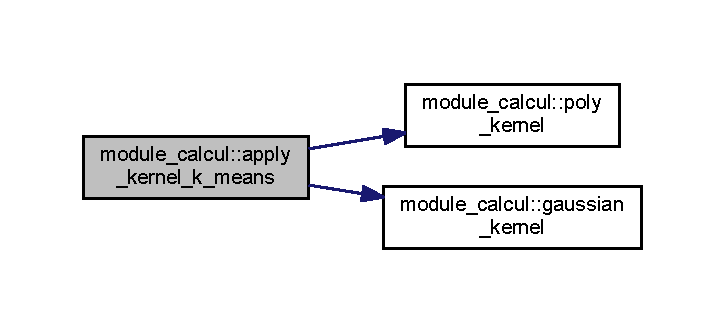
\includegraphics[width=348pt]{namespacemodule__calcul_a72848eb89fbd2fe4a97512f53752ca5c_cgraph}
\end{center}
\end{figure}


\hypertarget{namespacemodule__calcul_a7bf1a318c636b4e204f267103d00114a}{}\index{module\+\_\+calcul@{module\+\_\+calcul}!apply\+\_\+spectral\+\_\+clustering@{apply\+\_\+spectral\+\_\+clustering}}
\index{apply\+\_\+spectral\+\_\+clustering@{apply\+\_\+spectral\+\_\+clustering}!module\+\_\+calcul@{module\+\_\+calcul}}
\subsubsection[{apply\+\_\+spectral\+\_\+clustering}]{\setlength{\rightskip}{0pt plus 5cm}subroutine module\+\_\+calcul\+::apply\+\_\+spectral\+\_\+clustering (
\begin{DoxyParamCaption}
\item[{integer}]{proc\+\_\+id, }
\item[{integer}]{nb\+\_\+clusters\+\_\+max, }
\item[{integer}]{nb\+\_\+clusters\+\_\+opt, }
\item[{type({\bf type\+\_\+data})}]{partitioned\+\_\+data, }
\item[{double precision}]{sigma, }
\item[{type({\bf type\+\_\+clustering\+\_\+param})}]{clust\+\_\+param}
\end{DoxyParamCaption}
)}\label{namespacemodule__calcul_a7bf1a318c636b4e204f267103d00114a}


Here is the call graph for this function\+:\nopagebreak
\begin{figure}[H]
\begin{center}
\leavevmode
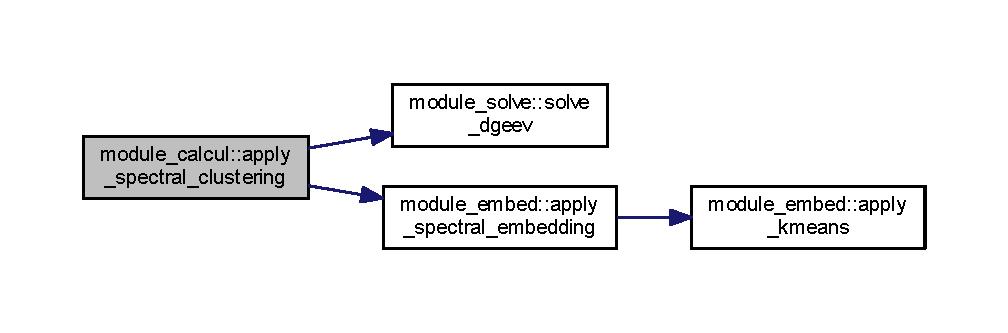
\includegraphics[width=350pt]{namespacemodule__calcul_a7bf1a318c636b4e204f267103d00114a_cgraph}
\end{center}
\end{figure}


\hypertarget{namespacemodule__calcul_a44b26b54d1b94dddba0ba575be04658b}{}\index{module\+\_\+calcul@{module\+\_\+calcul}!gaussian\+\_\+kernel@{gaussian\+\_\+kernel}}
\index{gaussian\+\_\+kernel@{gaussian\+\_\+kernel}!module\+\_\+calcul@{module\+\_\+calcul}}
\subsubsection[{gaussian\+\_\+kernel}]{\setlength{\rightskip}{0pt plus 5cm}double precision function, dimension(partitioned\+\_\+data\%nb,partitioned\+\_\+data\%nb) module\+\_\+calcul\+::gaussian\+\_\+kernel (
\begin{DoxyParamCaption}
\item[{type({\bf type\+\_\+data})}]{partitioned\+\_\+data, }
\item[{double precision}]{sigma}
\end{DoxyParamCaption}
)}\label{namespacemodule__calcul_a44b26b54d1b94dddba0ba575be04658b}


Here is the caller graph for this function\+:\nopagebreak
\begin{figure}[H]
\begin{center}
\leavevmode
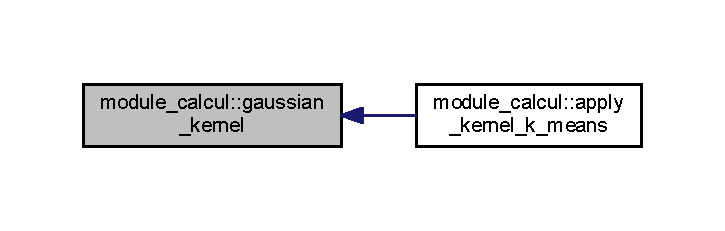
\includegraphics[width=348pt]{namespacemodule__calcul_a44b26b54d1b94dddba0ba575be04658b_icgraph}
\end{center}
\end{figure}


\hypertarget{namespacemodule__calcul_abd05b2b3ee81b4f779744a951d8a4c05}{}\index{module\+\_\+calcul@{module\+\_\+calcul}!get\+\_\+sigma@{get\+\_\+sigma}}
\index{get\+\_\+sigma@{get\+\_\+sigma}!module\+\_\+calcul@{module\+\_\+calcul}}
\subsubsection[{get\+\_\+sigma}]{\setlength{\rightskip}{0pt plus 5cm}subroutine module\+\_\+calcul\+::get\+\_\+sigma (
\begin{DoxyParamCaption}
\item[{type({\bf type\+\_\+data})}]{partitioned\+\_\+data, }
\item[{double precision}]{sigma}
\end{DoxyParamCaption}
)}\label{namespacemodule__calcul_abd05b2b3ee81b4f779744a951d8a4c05}


Computes the affinity parameter $sigma$. 

The Gaussian affinity matrix is widely used and depends on a free parameter $\sigma$. It is known that this parameter affects the results in spectral clustering and spectral embedding. With an assumption that the $p$ dimensionnal data set S composed of $n$ points is isotropic enough, this data set is included in a $p$ dimensional box bounded by $D_{max}$ the largest distance between pairs of points in $S$ \+: \begin{equation}D_{max} = \max_{1\leq i,j\leq n} \Vert x_i - x_j \Vert \end{equation} So a reference distance noted $\sigma$ could be defined. This distance represents the case of an uniform distribution in the sense that all pair of points are seprated by the same distance $\sigma$ in the box of edge size $D_{max}$ \+: \begin{equation}\sigma = \frac{D_{max}}{n^{1/p}} \end{equation} ~\newline
 This function is used to compute this parameter on one domain. The algorithm is simple \+: 
\begin{DoxyEnumerate}
\item {\bfseries  Find the maximum distance using two nested loops over the points in the domain }  
\item {\bfseries  Divide it by the $p^{th}$ root of $n$ }  
\end{DoxyEnumerate}
\begin{DoxyParams}[1]{Parameters}
\mbox{\tt in}  & {\em partitioned\+\_\+data} & the partitioned data for computing \\
\hline
\mbox{\tt out}  & {\em sigma} & the affinity parameter \\
\hline
\end{DoxyParams}


Here is the caller graph for this function\+:\nopagebreak
\begin{figure}[H]
\begin{center}
\leavevmode
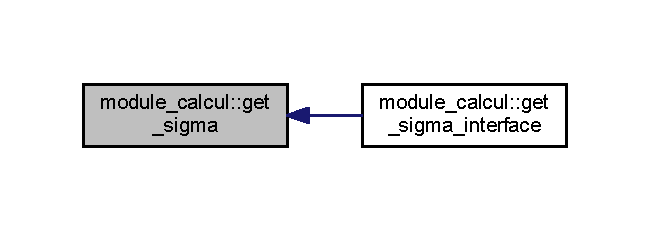
\includegraphics[width=312pt]{namespacemodule__calcul_abd05b2b3ee81b4f779744a951d8a4c05_icgraph}
\end{center}
\end{figure}


\hypertarget{namespacemodule__calcul_a118fd6a58b1064989fa68460457bea60}{}\index{module\+\_\+calcul@{module\+\_\+calcul}!get\+\_\+sigma\+\_\+interface@{get\+\_\+sigma\+\_\+interface}}
\index{get\+\_\+sigma\+\_\+interface@{get\+\_\+sigma\+\_\+interface}!module\+\_\+calcul@{module\+\_\+calcul}}
\subsubsection[{get\+\_\+sigma\+\_\+interface}]{\setlength{\rightskip}{0pt plus 5cm}subroutine module\+\_\+calcul\+::get\+\_\+sigma\+\_\+interface (
\begin{DoxyParamCaption}
\item[{integer}]{proc\+\_\+id, }
\item[{type({\bf type\+\_\+data})}]{partitioned\+\_\+data, }
\item[{double precision}]{sigma, }
\item[{double precision, dimension(\+:,\+:,\+:), pointer}]{bounds, }
\item[{integer, dimension(\+:), pointer}]{partitioning, }
\item[{double precision}]{epsilon}
\end{DoxyParamCaption}
)}\label{namespacemodule__calcul_a118fd6a58b1064989fa68460457bea60}


Computes the affinity parameter $sigma$ for the interface. 

This method is useful when the partitioning is made by interface. Because, the domain defining the interface has a volume whose topology changes drastically, a specific computation of $\sigma$ has to be made. \begin{DoxyRefDesc}{Deprecated}
\item[\hyperlink{deprecated__deprecated000001}{Deprecated}]Use \hyperlink{namespacemodule__calcul_abd05b2b3ee81b4f779744a951d8a4c05}{get\+\_\+sigma()} instead 
\begin{DoxyParams}[1]{Parameters}
\mbox{\tt in}  & {\em partitioned\+\_\+data} & the partitioned data for computing \\
\hline
\mbox{\tt in}  & {\em bounds} & the intervals along each dimension representing the bounds of each partition \\
\hline
\mbox{\tt in}  & {\em epsilon} & the slice thickness \\
\hline
\mbox{\tt in}  & {\em proc\+\_\+id} & the processus identifier \\
\hline
\mbox{\tt in}  & {\em partitioning} & the partitionning (number of processors along each dimension) \\
\hline
\mbox{\tt out}  & {\em sigma} & the affinity parameter \\
\hline
\end{DoxyParams}
\end{DoxyRefDesc}


Here is the call graph for this function\+:\nopagebreak
\begin{figure}[H]
\begin{center}
\leavevmode
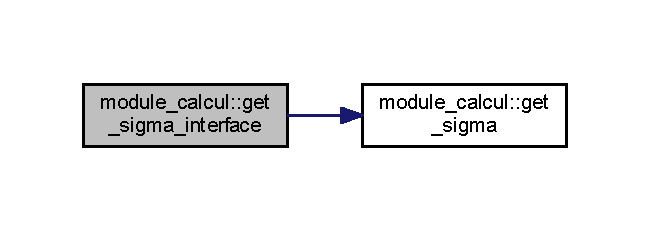
\includegraphics[width=312pt]{namespacemodule__calcul_a118fd6a58b1064989fa68460457bea60_cgraph}
\end{center}
\end{figure}


\hypertarget{namespacemodule__calcul_abb4a64b9f338e54274a250b9c10bf0bd}{}\index{module\+\_\+calcul@{module\+\_\+calcul}!mean\+\_\+shift@{mean\+\_\+shift}}
\index{mean\+\_\+shift@{mean\+\_\+shift}!module\+\_\+calcul@{module\+\_\+calcul}}
\subsubsection[{mean\+\_\+shift}]{\setlength{\rightskip}{0pt plus 5cm}subroutine module\+\_\+calcul\+::mean\+\_\+shift (
\begin{DoxyParamCaption}
\item[{integer}]{proc\+\_\+id, }
\item[{integer}]{nb\+\_\+clusters\+\_\+max, }
\item[{integer}]{nb\+\_\+clusters\+\_\+opt, }
\item[{type({\bf type\+\_\+data})}]{partitioned\+\_\+data, }
\item[{integer}]{bandwidth}
\end{DoxyParamCaption}
)}\label{namespacemodule__calcul_abb4a64b9f338e54274a250b9c10bf0bd}
\hypertarget{namespacemodule__calcul_a97fd8d0653adb9041ab3ca899c0d0f91}{}\index{module\+\_\+calcul@{module\+\_\+calcul}!poly\+\_\+kernel@{poly\+\_\+kernel}}
\index{poly\+\_\+kernel@{poly\+\_\+kernel}!module\+\_\+calcul@{module\+\_\+calcul}}
\subsubsection[{poly\+\_\+kernel}]{\setlength{\rightskip}{0pt plus 5cm}double precision function, dimension(partitioned\+\_\+data\%nb,partitioned\+\_\+data\%nb) module\+\_\+calcul\+::poly\+\_\+kernel (
\begin{DoxyParamCaption}
\item[{type({\bf type\+\_\+data})}]{partitioned\+\_\+data, }
\item[{double precision}]{gam, }
\item[{double precision}]{delta}
\end{DoxyParamCaption}
)}\label{namespacemodule__calcul_a97fd8d0653adb9041ab3ca899c0d0f91}


Here is the caller graph for this function\+:\nopagebreak
\begin{figure}[H]
\begin{center}
\leavevmode
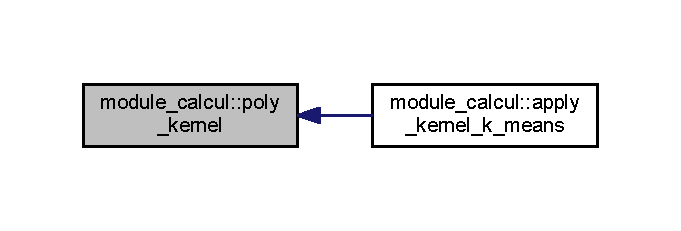
\includegraphics[width=327pt]{namespacemodule__calcul_a97fd8d0653adb9041ab3ca899c0d0f91_icgraph}
\end{center}
\end{figure}



\hypertarget{namespacemodule__decoupe}{}\section{module\+\_\+decoupe Module Reference}
\label{namespacemodule__decoupe}\index{module\+\_\+decoupe@{module\+\_\+decoupe}}


Contains methods enabling the partitionning and the groupping of the data.  


\subsection*{Functions/\+Subroutines}
\begin{DoxyCompactItemize}
\item 
subroutine \hyperlink{namespacemodule__decoupe_a20e9d554b6d62aa1aac7be71c223132e}{partition\+\_\+data} (data, epsilon, nb\+\_\+proc, coord\+\_\+min, coord\+\_\+max, partitioning, points\+\_\+by\+\_\+domain, assignements, bounds)
\begin{DoxyCompactList}\small\item\em Partitions the data into subdomains for a latter processing by the slaves. \end{DoxyCompactList}\item 
subroutine \hyperlink{namespacemodule__decoupe_ab1bd43de3891732cdf5803c4d86544dd}{define\+\_\+bounds} (data, coord\+\_\+min, coord\+\_\+max, bounds, partitioning, epsilon, nb\+\_\+proc)
\begin{DoxyCompactList}\small\item\em Defines the bounds of each subdomain. \end{DoxyCompactList}\item 
subroutine \hyperlink{namespacemodule__decoupe_afc4d3c1d1e2c287779200be5cf9d8205}{define\+\_\+domains} (nb\+\_\+proc, data, domains, bounds, partitioning)
\begin{DoxyCompactList}\small\item\em Defines the different subdomains. \end{DoxyCompactList}\item 
subroutine \hyperlink{namespacemodule__decoupe_a523f2f851f39859d9c60114c934b2d66}{partition\+\_\+with\+\_\+interface} (nb\+\_\+proc, data, points\+\_\+by\+\_\+domain, assignements, domains, epsilon)
\begin{DoxyCompactList}\small\item\em Partitions the data using interface. \end{DoxyCompactList}\item 
subroutine \hyperlink{namespacemodule__decoupe_a6f29dcc8367ffa44fa720260882fa04e}{partition\+\_\+with\+\_\+overlapping} (nb\+\_\+proc, data, points\+\_\+by\+\_\+domain, assignements, domains)
\begin{DoxyCompactList}\small\item\em Partitions the data using overlapping. \end{DoxyCompactList}\item 
subroutine \hyperlink{namespacemodule__decoupe_af5369423cd2f8c975e68cbc08c7b31c1}{group\+\_\+clusters} (nb\+\_\+clusters, points\+\_\+by\+\_\+cluster, cluster\+\_\+map, data)
\begin{DoxyCompactList}\small\item\em Groups the clusters and removes duplicates from the set of found clusters. \end{DoxyCompactList}\end{DoxyCompactItemize}


\subsection{Detailed Description}
Contains methods enabling the partitionning and the groupping of the data. 

\subsection{Function/\+Subroutine Documentation}
\hypertarget{namespacemodule__decoupe_ab1bd43de3891732cdf5803c4d86544dd}{}\index{module\+\_\+decoupe@{module\+\_\+decoupe}!define\+\_\+bounds@{define\+\_\+bounds}}
\index{define\+\_\+bounds@{define\+\_\+bounds}!module\+\_\+decoupe@{module\+\_\+decoupe}}
\subsubsection[{define\+\_\+bounds}]{\setlength{\rightskip}{0pt plus 5cm}subroutine module\+\_\+decoupe\+::define\+\_\+bounds (
\begin{DoxyParamCaption}
\item[{type({\bf type\+\_\+data})}]{data, }
\item[{double precision, dimension(\+:), pointer}]{coord\+\_\+min, }
\item[{double precision, dimension(\+:), pointer}]{coord\+\_\+max, }
\item[{double precision, dimension(\+:,\+:,\+:), pointer}]{bounds, }
\item[{integer, dimension(\+:), pointer}]{partitioning, }
\item[{double precision}]{epsilon, }
\item[{integer}]{nb\+\_\+proc}
\end{DoxyParamCaption}
)}\label{namespacemodule__decoupe_ab1bd43de3891732cdf5803c4d86544dd}


Defines the bounds of each subdomain. 

The output {\itshape bounds} has to be interpreted as follows\+: 
\begin{DoxyEnumerate}
\item The first index corresponds to the dimensions  
\item The second index corresponds to the partitioning along the dimension  
\item The third index corresponds to the extrema of the bounds  
\end{DoxyEnumerate}\begin{DoxyNote}{Note}
The bounds are composed of two points. 

In case of overlapping, the bounds overlapped each others. 
\end{DoxyNote}

\begin{DoxyParams}[1]{Parameters}
\mbox{\tt in}  & {\em data} & the entire data for computing \\
\hline
\mbox{\tt in}  & {\em epsilon} & the slice thickness \\
\hline
\mbox{\tt in}  & {\em nb\+\_\+proc} & the number of processors used \\
\hline
\mbox{\tt in}  & {\em partitioning} & the partitionning (number of processors along each dimension) \\
\hline
\mbox{\tt in,out}  & {\em coord\+\_\+max} & the maxima along each dimension of the data (coordinates) \\
\hline
\mbox{\tt in,out}  & {\em coord\+\_\+min} & the minima along each dimension of the data (coordinates) \\
\hline
\mbox{\tt out}  & {\em bounds} & the intervals along each dimension representing the bounds of each partition \\
\hline
\end{DoxyParams}


Here is the caller graph for this function\+:\nopagebreak
\begin{figure}[H]
\begin{center}
\leavevmode
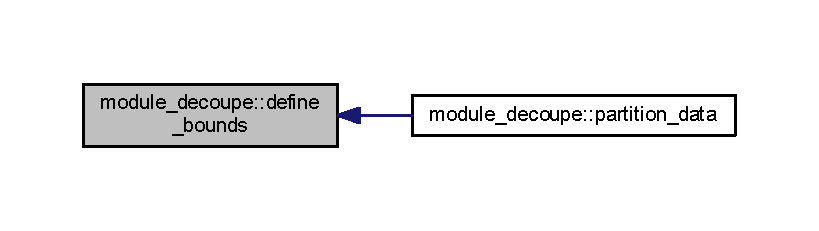
\includegraphics[width=350pt]{namespacemodule__decoupe_ab1bd43de3891732cdf5803c4d86544dd_icgraph}
\end{center}
\end{figure}


\hypertarget{namespacemodule__decoupe_afc4d3c1d1e2c287779200be5cf9d8205}{}\index{module\+\_\+decoupe@{module\+\_\+decoupe}!define\+\_\+domains@{define\+\_\+domains}}
\index{define\+\_\+domains@{define\+\_\+domains}!module\+\_\+decoupe@{module\+\_\+decoupe}}
\subsubsection[{define\+\_\+domains}]{\setlength{\rightskip}{0pt plus 5cm}subroutine module\+\_\+decoupe\+::define\+\_\+domains (
\begin{DoxyParamCaption}
\item[{integer}]{nb\+\_\+proc, }
\item[{type({\bf type\+\_\+data})}]{data, }
\item[{double precision, dimension(\+:,\+:,\+:), pointer}]{domains, }
\item[{double precision, dimension(\+:,\+:,\+:), pointer}]{bounds, }
\item[{integer, dimension(\+:), pointer}]{partitioning}
\end{DoxyParamCaption}
)}\label{namespacemodule__decoupe_afc4d3c1d1e2c287779200be5cf9d8205}


Defines the different subdomains. 

The output {\itshape domains} has to be interpreted as follows\+: 
\begin{DoxyEnumerate}
\item The first index corresponds to the domain id 
\item The second index corresponds to the dimensions  
\item The third index corresponds to the extrema of the bounds  
\end{DoxyEnumerate}\begin{DoxySeeAlso}{See also}
\hyperlink{namespacemodule__decoupe_ab1bd43de3891732cdf5803c4d86544dd}{define\+\_\+bounds()} 
\end{DoxySeeAlso}

\begin{DoxyParams}[1]{Parameters}
\mbox{\tt in}  & {\em data} & the entire data for computing \\
\hline
\mbox{\tt in}  & {\em bounds} & the intervals along each dimension representing the bounds of each partition \\
\hline
\mbox{\tt in}  & {\em nb\+\_\+proc} & the number of processors used \\
\hline
\mbox{\tt in}  & {\em partitioning} & the partitionning (number of processors along each dimension) \\
\hline
\mbox{\tt out}  & {\em domains} & the domains constructed from the bounds \\
\hline
\end{DoxyParams}


Here is the caller graph for this function\+:\nopagebreak
\begin{figure}[H]
\begin{center}
\leavevmode
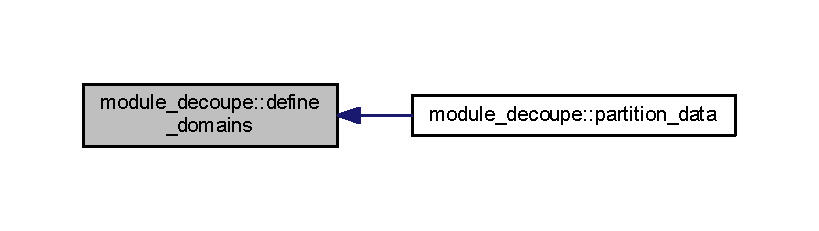
\includegraphics[width=350pt]{namespacemodule__decoupe_afc4d3c1d1e2c287779200be5cf9d8205_icgraph}
\end{center}
\end{figure}


\hypertarget{namespacemodule__decoupe_af5369423cd2f8c975e68cbc08c7b31c1}{}\index{module\+\_\+decoupe@{module\+\_\+decoupe}!group\+\_\+clusters@{group\+\_\+clusters}}
\index{group\+\_\+clusters@{group\+\_\+clusters}!module\+\_\+decoupe@{module\+\_\+decoupe}}
\subsubsection[{group\+\_\+clusters}]{\setlength{\rightskip}{0pt plus 5cm}subroutine module\+\_\+decoupe\+::group\+\_\+clusters (
\begin{DoxyParamCaption}
\item[{integer}]{nb\+\_\+clusters, }
\item[{integer, dimension(\+:), pointer}]{points\+\_\+by\+\_\+cluster, }
\item[{integer, dimension(\+:,\+:), pointer}]{cluster\+\_\+map, }
\item[{type({\bf type\+\_\+data})}]{data}
\end{DoxyParamCaption}
)}\label{namespacemodule__decoupe_af5369423cd2f8c975e68cbc08c7b31c1}


Groups the clusters and removes duplicates from the set of found clusters. 

The method operates on all the computed clusters and when an intersection is found between two of them (at least one point in common), they are melted. 
\begin{DoxyParams}[1]{Parameters}
\mbox{\tt in}  & {\em nb\+\_\+clusters} & the number of clusters \\
\hline
\mbox{\tt in}  & {\em nb\+\_\+clusters} & the number of clusters \\
\hline
\mbox{\tt in}  & {\em nb\+\_\+clusters} & the number of clusters \\
\hline
\mbox{\tt in,out}  & {\em cluster\+\_\+map} & the cluster indices and the number of points in each cluster \\
\hline
\mbox{\tt in,out}  & {\em points\+\_\+by\+\_\+cluster} & the number of points in each cluster \\
\hline
\mbox{\tt out}  & {\em data} & the entire data for computing \\
\hline
\end{DoxyParams}
\hypertarget{namespacemodule__decoupe_a20e9d554b6d62aa1aac7be71c223132e}{}\index{module\+\_\+decoupe@{module\+\_\+decoupe}!partition\+\_\+data@{partition\+\_\+data}}
\index{partition\+\_\+data@{partition\+\_\+data}!module\+\_\+decoupe@{module\+\_\+decoupe}}
\subsubsection[{partition\+\_\+data}]{\setlength{\rightskip}{0pt plus 5cm}subroutine module\+\_\+decoupe\+::partition\+\_\+data (
\begin{DoxyParamCaption}
\item[{type({\bf type\+\_\+data})}]{data, }
\item[{double precision}]{epsilon, }
\item[{integer}]{nb\+\_\+proc, }
\item[{double precision, dimension(\+:), pointer}]{coord\+\_\+min, }
\item[{double precision, dimension(\+:), pointer}]{coord\+\_\+max, }
\item[{integer, dimension(\+:), pointer}]{partitioning, }
\item[{integer, dimension(\+:), pointer}]{points\+\_\+by\+\_\+domain, }
\item[{integer, dimension(\+:,\+:), pointer}]{assignements, }
\item[{double precision, dimension(\+:,\+:,\+:), pointer}]{bounds}
\end{DoxyParamCaption}
)}\label{namespacemodule__decoupe_a20e9d554b6d62aa1aac7be71c223132e}


Partitions the data into subdomains for a latter processing by the slaves. 

The following is performed \+: 
\begin{DoxyEnumerate}
\item The bounds of each domain are defined (see \hyperlink{namespacemodule__decoupe_ab1bd43de3891732cdf5803c4d86544dd}{define\+\_\+bounds()}). 
\item The domains are defined using the bounds (see \hyperlink{namespacemodule__decoupe_afc4d3c1d1e2c287779200be5cf9d8205}{define\+\_\+domains()}). 
\item The domains are written in a dedicated file (see \hyperlink{namespacemodule__sortie_a835f7338c29161d6893c6bbddf4174f4}{write\+\_\+domains()}). 
\item The data is partitioned using interface or overlapping (see \hyperlink{namespacemodule__decoupe_a523f2f851f39859d9c60114c934b2d66}{partition\+\_\+with\+\_\+interface()} and \hyperlink{namespacemodule__decoupe_a6f29dcc8367ffa44fa720260882fa04e}{partition\+\_\+with\+\_\+overlapping()}). 
\item The partitioning is written in dedicated files (see \hyperlink{namespacemodule__sortie_abd1cdf529e5c71b3186c8d980e3d5117}{write\+\_\+partitioning()}). 
\end{DoxyEnumerate}
\begin{DoxyParams}[1]{Parameters}
\mbox{\tt in}  & {\em data} & the entire data for computing \\
\hline
\mbox{\tt in}  & {\em epsilon} & the slice thickness \\
\hline
\mbox{\tt in}  & {\em nb\+\_\+proc} & the number of processors used \\
\hline
\mbox{\tt in}  & {\em partitioning} & the partitionning (number of processors along each dimension) \\
\hline
\mbox{\tt in,out}  & {\em coord\+\_\+max} & the maxima along each dimension of the data (coordinates) \\
\hline
\mbox{\tt in,out}  & {\em coord\+\_\+min} & the minima along each dimension of the data (coordinates) \\
\hline
\mbox{\tt out}  & {\em bounds} & the intervals along each dimension representing the bounds of each partition \\
\hline
\mbox{\tt out}  & {\em assignements} & the assignement of each point in a partition \\
\hline
\mbox{\tt out}  & {\em points\+\_\+by\+\_\+domain} & the number of points in each partition \\
\hline
\end{DoxyParams}


Here is the call graph for this function\+:\nopagebreak
\begin{figure}[H]
\begin{center}
\leavevmode
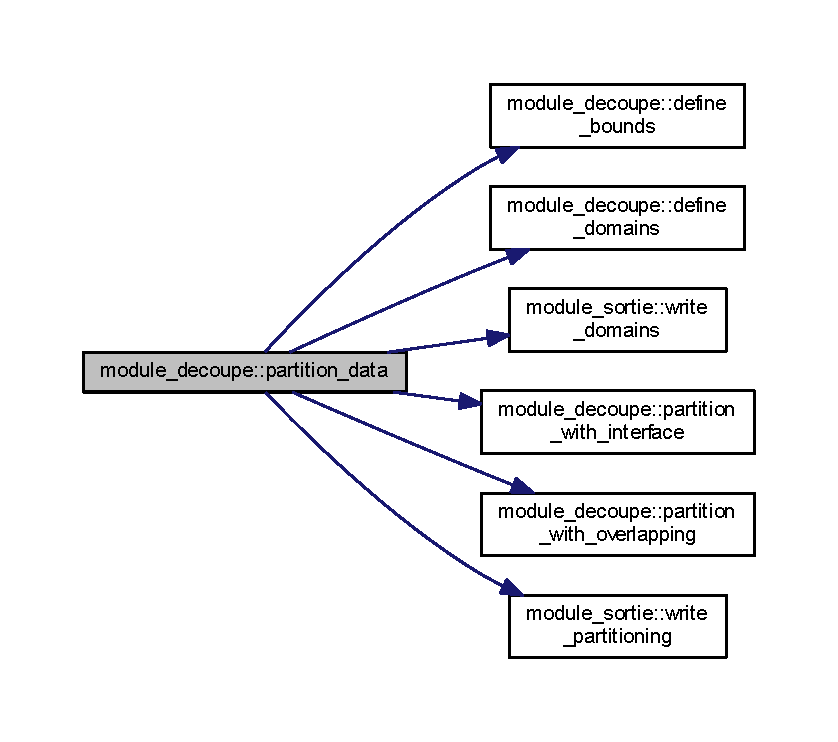
\includegraphics[width=350pt]{namespacemodule__decoupe_a20e9d554b6d62aa1aac7be71c223132e_cgraph}
\end{center}
\end{figure}


\hypertarget{namespacemodule__decoupe_a523f2f851f39859d9c60114c934b2d66}{}\index{module\+\_\+decoupe@{module\+\_\+decoupe}!partition\+\_\+with\+\_\+interface@{partition\+\_\+with\+\_\+interface}}
\index{partition\+\_\+with\+\_\+interface@{partition\+\_\+with\+\_\+interface}!module\+\_\+decoupe@{module\+\_\+decoupe}}
\subsubsection[{partition\+\_\+with\+\_\+interface}]{\setlength{\rightskip}{0pt plus 5cm}subroutine module\+\_\+decoupe\+::partition\+\_\+with\+\_\+interface (
\begin{DoxyParamCaption}
\item[{integer}]{nb\+\_\+proc, }
\item[{type({\bf type\+\_\+data})}]{data, }
\item[{integer, dimension(\+:), pointer}]{points\+\_\+by\+\_\+domain, }
\item[{integer, dimension(\+:,\+:), pointer}]{assignements, }
\item[{double precision, dimension(\+:,\+:,\+:), pointer}]{domains, }
\item[{double precision}]{epsilon}
\end{DoxyParamCaption}
)}\label{namespacemodule__decoupe_a523f2f851f39859d9c60114c934b2d66}


Partitions the data using interface. 

The method partitions the entire data by defining which point belongs to which domain. It consists of a loop on all the point in data set. Then it \char`\"{}fills\char`\"{} the domains one after another using a nested loop. When a point does not fit the bounds define in the input {\itshape domains}, the algorithm switch to the next domain. Finally, an extra domain is defined (the interface) which corresponds to the area around the bounds with a predefined slice thickness. \begin{DoxySeeAlso}{See also}
\hyperlink{namespacemodule__decoupe_a6f29dcc8367ffa44fa720260882fa04e}{partition\+\_\+with\+\_\+overlapping()} 
\end{DoxySeeAlso}

\begin{DoxyParams}[1]{Parameters}
\mbox{\tt in}  & {\em data} & the entire data for computing \\
\hline
\mbox{\tt in}  & {\em domains} & the domains constructed from the bounds \\
\hline
\mbox{\tt in}  & {\em epsilon} & the slice thickness \\
\hline
\mbox{\tt in}  & {\em nb\+\_\+proc} & the number of processors used \\
\hline
\mbox{\tt out}  & {\em assignements} & the assignement of each point in a partition \\
\hline
\mbox{\tt out}  & {\em points\+\_\+by\+\_\+domain} & the number of points in each partition \\
\hline
\end{DoxyParams}


Here is the caller graph for this function\+:\nopagebreak
\begin{figure}[H]
\begin{center}
\leavevmode
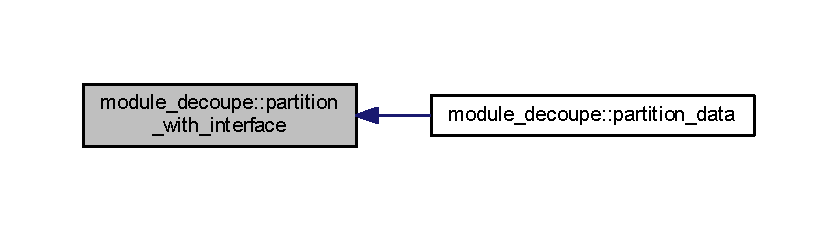
\includegraphics[width=350pt]{namespacemodule__decoupe_a523f2f851f39859d9c60114c934b2d66_icgraph}
\end{center}
\end{figure}


\hypertarget{namespacemodule__decoupe_a6f29dcc8367ffa44fa720260882fa04e}{}\index{module\+\_\+decoupe@{module\+\_\+decoupe}!partition\+\_\+with\+\_\+overlapping@{partition\+\_\+with\+\_\+overlapping}}
\index{partition\+\_\+with\+\_\+overlapping@{partition\+\_\+with\+\_\+overlapping}!module\+\_\+decoupe@{module\+\_\+decoupe}}
\subsubsection[{partition\+\_\+with\+\_\+overlapping}]{\setlength{\rightskip}{0pt plus 5cm}subroutine module\+\_\+decoupe\+::partition\+\_\+with\+\_\+overlapping (
\begin{DoxyParamCaption}
\item[{integer}]{nb\+\_\+proc, }
\item[{type({\bf type\+\_\+data})}]{data, }
\item[{integer, dimension(\+:), pointer}]{points\+\_\+by\+\_\+domain, }
\item[{integer, dimension(\+:,\+:), pointer}]{assignements, }
\item[{double precision, dimension(\+:,\+:,\+:), pointer}]{domains}
\end{DoxyParamCaption}
)}\label{namespacemodule__decoupe_a6f29dcc8367ffa44fa720260882fa04e}


Partitions the data using overlapping. 

The method partitions the entire data by defining which point belongs to which domain. It consists of two nested loop. The first one on the points and the second one on the domains (ie the processes). For each point, it checks if it fits the bounds defined in the input {\itshape domains} (and that for each domain) and in that case add to it. \begin{DoxyNote}{Note}
Some points will be present in different domains. 
\end{DoxyNote}
\begin{DoxySeeAlso}{See also}
\hyperlink{namespacemodule__decoupe_a523f2f851f39859d9c60114c934b2d66}{partition\+\_\+with\+\_\+interface()} 
\end{DoxySeeAlso}

\begin{DoxyParams}[1]{Parameters}
\mbox{\tt in}  & {\em data} & the entire data for computing \\
\hline
\mbox{\tt in}  & {\em domains} & the domains constructed from the bounds \\
\hline
\mbox{\tt in}  & {\em nb\+\_\+proc} & the number of processors used \\
\hline
\mbox{\tt out}  & {\em assignements} & the assignement of each point in a partition \\
\hline
\mbox{\tt out}  & {\em points\+\_\+by\+\_\+domain} & the number of points in each partition \\
\hline
\end{DoxyParams}


Here is the caller graph for this function\+:\nopagebreak
\begin{figure}[H]
\begin{center}
\leavevmode
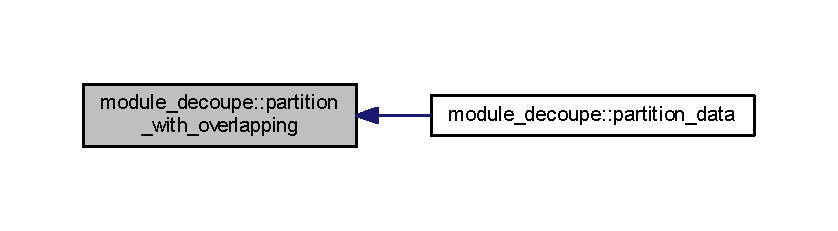
\includegraphics[width=350pt]{namespacemodule__decoupe_a6f29dcc8367ffa44fa720260882fa04e_icgraph}
\end{center}
\end{figure}



\hypertarget{namespacemodule__embed}{}\section{module\+\_\+embed Module Reference}
\label{namespacemodule__embed}\index{module\+\_\+embed@{module\+\_\+embed}}


Contains K-\/means and spectral embedding algorithms.  


\subsection*{Functions/\+Subroutines}
\begin{DoxyCompactItemize}
\item 
subroutine \hyperlink{namespacemodule__embed_ab78350f96b04d0ce2ca0bd10abd50440}{apply\+\_\+spectral\+\_\+embedding} (nb\+\_\+clusters, n, Z, A, ratio, clusters, clusters\+\_\+centers, points\+\_\+by\+\_\+clusters, clusters\+\_\+energies, nb\+\_\+info, proc\+\_\+id, ratio\+\_\+moy, ratio\+\_\+rij, ratio\+\_\+rii)
\begin{DoxyCompactList}\small\item\em Computes the clusters using eigen vector matrix. \end{DoxyCompactList}\item 
subroutine \hyperlink{namespacemodule__embed_a27f0555abee781e67c2def5e2b9471d2}{apply\+\_\+kmeans} (dim, nb\+\_\+points, nb\+\_\+clusters, nb\+\_\+iter\+\_\+max, nb\+\_\+iter, points, clusters, clusters\+\_\+centers, points\+\_\+by\+\_\+clusters, clusters\+\_\+energies, proc\+\_\+id)
\begin{DoxyCompactList}\small\item\em Implements K-\/\+Means algorithm (required by spectral clustering and Kernel K-\/\+Means methods) The algorithm works as follows\+: \end{DoxyCompactList}\end{DoxyCompactItemize}


\subsection{Detailed Description}
Contains K-\/means and spectral embedding algorithms. 

\subsection{Function/\+Subroutine Documentation}
\hypertarget{namespacemodule__embed_a27f0555abee781e67c2def5e2b9471d2}{}\index{module\+\_\+embed@{module\+\_\+embed}!apply\+\_\+kmeans@{apply\+\_\+kmeans}}
\index{apply\+\_\+kmeans@{apply\+\_\+kmeans}!module\+\_\+embed@{module\+\_\+embed}}
\subsubsection[{apply\+\_\+kmeans}]{\setlength{\rightskip}{0pt plus 5cm}subroutine module\+\_\+embed\+::apply\+\_\+kmeans (
\begin{DoxyParamCaption}
\item[{integer}]{dim, }
\item[{integer}]{nb\+\_\+points, }
\item[{integer}]{nb\+\_\+clusters, }
\item[{integer}]{nb\+\_\+iter\+\_\+max, }
\item[{integer}]{nb\+\_\+iter, }
\item[{double precision, dimension (dim, nb\+\_\+points)}]{points, }
\item[{integer, dimension (nb\+\_\+points)}]{clusters, }
\item[{double precision, dimension (dim, nb\+\_\+clusters)}]{clusters\+\_\+centers, }
\item[{integer, dimension (nb\+\_\+clusters)}]{points\+\_\+by\+\_\+clusters, }
\item[{double precision, dimension (nb\+\_\+clusters)}]{clusters\+\_\+energies, }
\item[{integer}]{proc\+\_\+id}
\end{DoxyParamCaption}
)}\label{namespacemodule__embed_a27f0555abee781e67c2def5e2b9471d2}


Implements K-\/\+Means algorithm (required by spectral clustering and Kernel K-\/\+Means methods) The algorithm works as follows\+: 


\begin{DoxyEnumerate}
\item Choose {\itshape nb\+\_\+clusters} starting points as cluster centers randomly 
\item For each point in the data set, find the minimum distance from a cluster center and attach it to the corresponding cluster 
\item Compute the density center of each cluster 
\item Stop if the density centers are similar to the cluster centers 
\item Select the density centers as new cluster centers and start from the beginning 
\end{DoxyEnumerate}
\begin{DoxyParams}[1]{Parameters}
\mbox{\tt in}  & {\em points} & the points \\
\hline
\mbox{\tt in}  & {\em dim} & the number of spatial dimensions \\
\hline
\mbox{\tt in}  & {\em dim} & the number of spatial dimensions \\
\hline
\mbox{\tt in}  & {\em dim} & \\
\hline
\mbox{\tt in}  & {\em nb\+\_\+clusters} & the number of clusters \\
\hline
\mbox{\tt in}  & {\em nb\+\_\+clusters} & the number of clusters \\
\hline
\mbox{\tt in}  & {\em nb\+\_\+clusters} & the number of clusters \\
\hline
\mbox{\tt in}  & {\em nb\+\_\+iter\+\_\+max} & the maximum number of iterations \\
\hline
\mbox{\tt in}  & {\em nb\+\_\+points} & the number of points \\
\hline
\mbox{\tt in}  & {\em nb\+\_\+points} & the number of points \\
\hline
\mbox{\tt in,out}  & {\em clusters\+\_\+centers} & the cluster centers \\
\hline
 & {\em proc\+\_\+id} & the processus identifier \\
\hline
\mbox{\tt out}  & {\em clusters\+\_\+energies} & the cluster energies \\
\hline
\mbox{\tt out}  & {\em nb\+\_\+iter} & the number of iterations taken \\
\hline
\mbox{\tt out}  & {\em clusters} & indicates which cluster each point belongs to \\
\hline
\mbox{\tt out}  & {\em points\+\_\+by\+\_\+clusters} & the number of points in each cluster \\
\hline
\end{DoxyParams}


Here is the caller graph for this function\+:\nopagebreak
\begin{figure}[H]
\begin{center}
\leavevmode
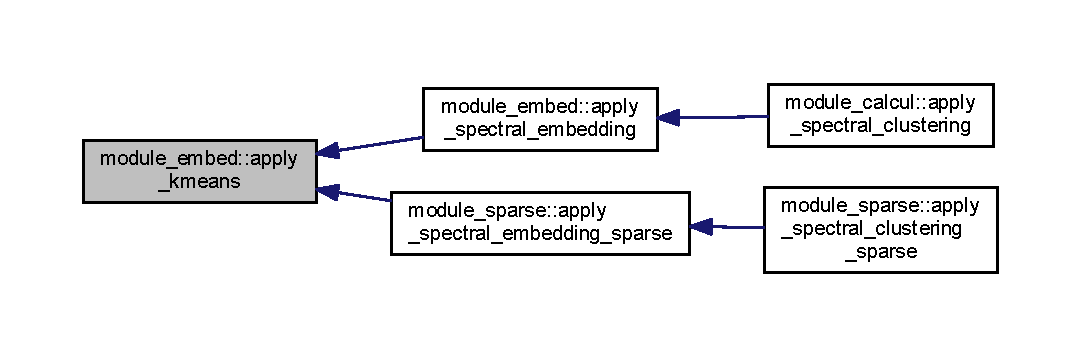
\includegraphics[width=350pt]{namespacemodule__embed_a27f0555abee781e67c2def5e2b9471d2_icgraph}
\end{center}
\end{figure}


\hypertarget{namespacemodule__embed_ab78350f96b04d0ce2ca0bd10abd50440}{}\index{module\+\_\+embed@{module\+\_\+embed}!apply\+\_\+spectral\+\_\+embedding@{apply\+\_\+spectral\+\_\+embedding}}
\index{apply\+\_\+spectral\+\_\+embedding@{apply\+\_\+spectral\+\_\+embedding}!module\+\_\+embed@{module\+\_\+embed}}
\subsubsection[{apply\+\_\+spectral\+\_\+embedding}]{\setlength{\rightskip}{0pt plus 5cm}subroutine module\+\_\+embed\+::apply\+\_\+spectral\+\_\+embedding (
\begin{DoxyParamCaption}
\item[{integer}]{nb\+\_\+clusters, }
\item[{integer}]{n, }
\item[{double precision, dimension(\+:,\+:), pointer}]{Z, }
\item[{double precision, dimension(\+:,\+:), pointer}]{A, }
\item[{double precision}]{ratio, }
\item[{integer, dimension(\+:), pointer}]{clusters, }
\item[{double precision, dimension(\+:,\+:), pointer}]{clusters\+\_\+centers, }
\item[{integer, dimension(\+:), pointer}]{points\+\_\+by\+\_\+clusters, }
\item[{double precision, dimension(\+:), pointer}]{clusters\+\_\+energies, }
\item[{integer}]{nb\+\_\+info, }
\item[{integer}]{proc\+\_\+id, }
\item[{double precision}]{ratio\+\_\+moy, }
\item[{double precision}]{ratio\+\_\+rij, }
\item[{double precision}]{ratio\+\_\+rii}
\end{DoxyParamCaption}
)}\label{namespacemodule__embed_ab78350f96b04d0ce2ca0bd10abd50440}


Computes the clusters using eigen vector matrix. 

The first part of the method performs the following\+: 
\begin{DoxyEnumerate}
\item Extract the {\itshape nb\+\_\+clusters} first columns of the eigen vector matrix (corresponding to the highest eigen values) 
\item Normalize the matrix and transposes it  
\item Apply K-\/\+Means on it to find the clusters  
\end{DoxyEnumerate}Then it operates a quality measurement on the found clusters. It computes the sum of the ratios that indicate if the number of clusters is optimal. The lower this sum is, the best is the number of clusters. This method also compute the number of clusters that have at least one point and that have an internal affinity greater than zero. \begin{DoxyNote}{Note}
We refer you to the article {\itshape \char`\"{}\+On a strategy for Spectral Clustering with parallel computation\char`\"{}} for a better understanding. 
\end{DoxyNote}

\begin{DoxyParams}[1]{Parameters}
\mbox{\tt in}  & {\em A} & the affinity matrix \\
\hline
\mbox{\tt in}  & {\em Z} & the matrix of eigen vectors \\
\hline
\mbox{\tt in}  & {\em n} & \\
\hline
\mbox{\tt in}  & {\em nb\+\_\+clusters} & the number of clusters \\
\hline
\mbox{\tt in}  & {\em nb\+\_\+clusters} & the number of clusters \\
\hline
\mbox{\tt in}  & {\em nb\+\_\+clusters} & the number of clusters \\
\hline
\mbox{\tt in}  & {\em proc\+\_\+id} & the processus identifier \\
\hline
\mbox{\tt out}  & {\em clusters\+\_\+centers} & the cluster centers \\
\hline
\mbox{\tt out}  & {\em clusters\+\_\+energies} & the cluster energies \\
\hline
\mbox{\tt out}  & {\em ratio} & the sum of the ratios between Frobenius norm of the off-\/diagonal and the diagonal blocks of the normalized affinity matrix \\
\hline
\mbox{\tt out}  & {\em ratio\+\_\+moy} & \\
\hline
\mbox{\tt out}  & {\em ratio\+\_\+rii} & the sum of the denominator of each ratio \\
\hline
\mbox{\tt out}  & {\em ratio\+\_\+rij} & the sum of the numerators of each ratio \\
\hline
\mbox{\tt out}  & {\em nb\+\_\+info} & the reduced number of clusters (?) \\
\hline
\mbox{\tt out}  & {\em clusters} & indicates which cluster each point belongs to \\
\hline
\mbox{\tt out}  & {\em points\+\_\+by\+\_\+clusters} & the number of points in each cluster \\
\hline
\end{DoxyParams}


Here is the call graph for this function\+:\nopagebreak
\begin{figure}[H]
\begin{center}
\leavevmode
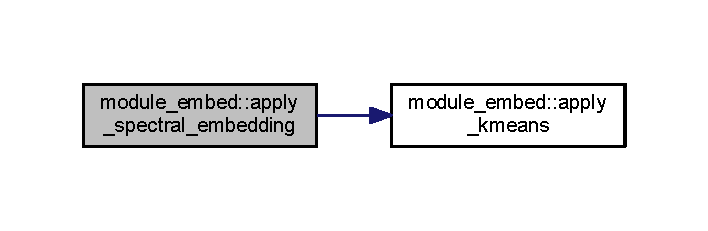
\includegraphics[width=340pt]{namespacemodule__embed_ab78350f96b04d0ce2ca0bd10abd50440_cgraph}
\end{center}
\end{figure}




Here is the caller graph for this function\+:\nopagebreak
\begin{figure}[H]
\begin{center}
\leavevmode
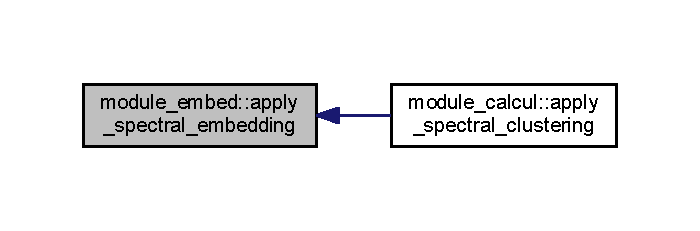
\includegraphics[width=336pt]{namespacemodule__embed_ab78350f96b04d0ce2ca0bd10abd50440_icgraph}
\end{center}
\end{figure}



\hypertarget{namespacemodule__entree}{}\section{module\+\_\+entree Module Reference}
\label{namespacemodule__entree}\index{module\+\_\+entree@{module\+\_\+entree}}


Contains methods enabling data and parameter file reading.  


\subsection*{Functions/\+Subroutines}
\begin{DoxyCompactItemize}
\item 
subroutine \hyperlink{namespacemodule__entree_ae91fc1d896afb27c01d7314dce81db70}{help}
\begin{DoxyCompactList}\small\item\em Displays help on used formats and keywords for {\itshape param.\+in} file. \end{DoxyCompactList}\item 
subroutine \hyperlink{namespacemodule__entree_a4a8eec4484896ca8cb249548e1cf537f}{read\+\_\+params} (data, epsilon, coord\+\_\+min, coord\+\_\+max, nb\+\_\+proc, partitioning, input\+\_\+file, sigma, nb\+\_\+clusters\+\_\+max, list\+\_\+nb\+\_\+clusters, clust\+\_\+param)
\begin{DoxyCompactList}\small\item\em Reads a file in which there is the whole information on the data. \end{DoxyCompactList}\item 
subroutine \hyperlink{namespacemodule__entree_a93d220ea64cd5e1d155255bca188de0c}{read\+\_\+coordinates\+\_\+data} (input\+\_\+file, data, coord\+\_\+min, coord\+\_\+max)
\begin{DoxyCompactList}\small\item\em Reads data written in coordinates format. \end{DoxyCompactList}\item 
subroutine \hyperlink{namespacemodule__entree_aaa0e9ef36218a32292aa65a9b8602cda}{read\+\_\+picture\+\_\+data} (input\+\_\+file, data, coord\+\_\+min, coord\+\_\+max)
\begin{DoxyCompactList}\small\item\em Reads data written in picture format. \end{DoxyCompactList}\item 
subroutine \hyperlink{namespacemodule__entree_ae5047aaa626b5cac3c9f98267f502669}{read\+\_\+geometric\+\_\+data} (input\+\_\+file, data, coord\+\_\+min, coord\+\_\+max)
\begin{DoxyCompactList}\small\item\em Reads data written in geometric format. \end{DoxyCompactList}\item 
subroutine \hyperlink{namespacemodule__entree_a25df009403bc610c2ef3b3a151574979}{read\+\_\+threshold\+\_\+data} (input\+\_\+file, data, coord\+\_\+min, coord\+\_\+max)
\begin{DoxyCompactList}\small\item\em Reads data written in threshold format. \end{DoxyCompactList}\item 
subroutine \hyperlink{namespacemodule__entree_a08bc5eb1225bf568c94df30b22f04e03}{assign\+\_\+picture\+\_\+array} (data)
\begin{DoxyCompactList}\small\item\em Puts the index number of the pixels into an array. \end{DoxyCompactList}\end{DoxyCompactItemize}


\subsection{Detailed Description}
Contains methods enabling data and parameter file reading. 

\subsection{Function/\+Subroutine Documentation}
\hypertarget{namespacemodule__entree_a08bc5eb1225bf568c94df30b22f04e03}{}\index{module\+\_\+entree@{module\+\_\+entree}!assign\+\_\+picture\+\_\+array@{assign\+\_\+picture\+\_\+array}}
\index{assign\+\_\+picture\+\_\+array@{assign\+\_\+picture\+\_\+array}!module\+\_\+entree@{module\+\_\+entree}}
\subsubsection[{assign\+\_\+picture\+\_\+array}]{\setlength{\rightskip}{0pt plus 5cm}subroutine module\+\_\+entree\+::assign\+\_\+picture\+\_\+array (
\begin{DoxyParamCaption}
\item[{type({\bf type\+\_\+data})}]{data}
\end{DoxyParamCaption}
)}\label{namespacemodule__entree_a08bc5eb1225bf568c94df30b22f04e03}


Puts the index number of the pixels into an array. 

Each point of the data set is mapped to an array corresponding to an image. Thus, instead of one index for accessing one point, two will be used (row and column). 
\begin{DoxyParams}[1]{Parameters}
\mbox{\tt in,out}  & {\em data} & the entire data for computing \\
\hline
\end{DoxyParams}


Here is the caller graph for this function\+:\nopagebreak
\begin{figure}[H]
\begin{center}
\leavevmode
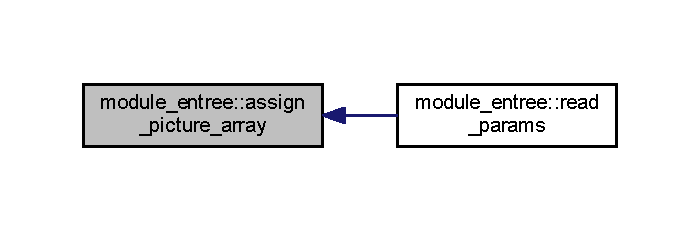
\includegraphics[width=336pt]{namespacemodule__entree_a08bc5eb1225bf568c94df30b22f04e03_icgraph}
\end{center}
\end{figure}


\hypertarget{namespacemodule__entree_ae91fc1d896afb27c01d7314dce81db70}{}\index{module\+\_\+entree@{module\+\_\+entree}!help@{help}}
\index{help@{help}!module\+\_\+entree@{module\+\_\+entree}}
\subsubsection[{help}]{\setlength{\rightskip}{0pt plus 5cm}subroutine module\+\_\+entree\+::help (
\begin{DoxyParamCaption}
{}
\end{DoxyParamCaption}
)}\label{namespacemodule__entree_ae91fc1d896afb27c01d7314dce81db70}


Displays help on used formats and keywords for {\itshape param.\+in} file. 



Here is the caller graph for this function\+:\nopagebreak
\begin{figure}[H]
\begin{center}
\leavevmode
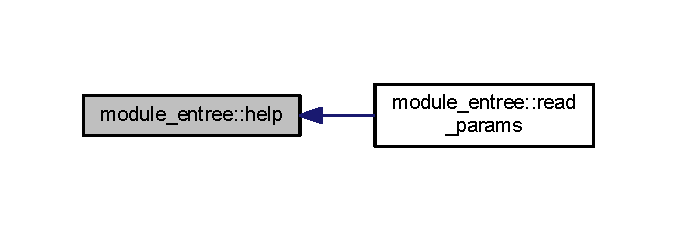
\includegraphics[width=325pt]{namespacemodule__entree_ae91fc1d896afb27c01d7314dce81db70_icgraph}
\end{center}
\end{figure}


\hypertarget{namespacemodule__entree_a93d220ea64cd5e1d155255bca188de0c}{}\index{module\+\_\+entree@{module\+\_\+entree}!read\+\_\+coordinates\+\_\+data@{read\+\_\+coordinates\+\_\+data}}
\index{read\+\_\+coordinates\+\_\+data@{read\+\_\+coordinates\+\_\+data}!module\+\_\+entree@{module\+\_\+entree}}
\subsubsection[{read\+\_\+coordinates\+\_\+data}]{\setlength{\rightskip}{0pt plus 5cm}subroutine module\+\_\+entree\+::read\+\_\+coordinates\+\_\+data (
\begin{DoxyParamCaption}
\item[{character (len=30)}]{input\+\_\+file, }
\item[{type({\bf type\+\_\+data})}]{data, }
\item[{double precision, dimension(\+:), pointer}]{coord\+\_\+min, }
\item[{double precision, dimension(\+:), pointer}]{coord\+\_\+max}
\end{DoxyParamCaption}
)}\label{namespacemodule__entree_a93d220ea64cd5e1d155255bca188de0c}


Reads data written in coordinates format. 



Here is the caller graph for this function\+:\nopagebreak
\begin{figure}[H]
\begin{center}
\leavevmode
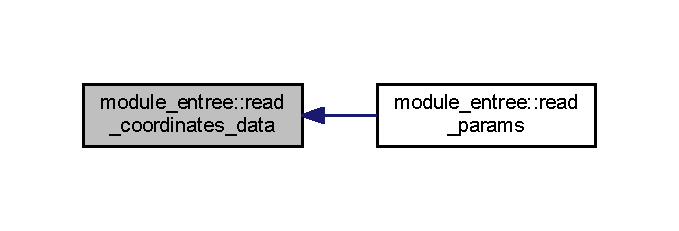
\includegraphics[width=326pt]{namespacemodule__entree_a93d220ea64cd5e1d155255bca188de0c_icgraph}
\end{center}
\end{figure}


\hypertarget{namespacemodule__entree_ae5047aaa626b5cac3c9f98267f502669}{}\index{module\+\_\+entree@{module\+\_\+entree}!read\+\_\+geometric\+\_\+data@{read\+\_\+geometric\+\_\+data}}
\index{read\+\_\+geometric\+\_\+data@{read\+\_\+geometric\+\_\+data}!module\+\_\+entree@{module\+\_\+entree}}
\subsubsection[{read\+\_\+geometric\+\_\+data}]{\setlength{\rightskip}{0pt plus 5cm}subroutine module\+\_\+entree\+::read\+\_\+geometric\+\_\+data (
\begin{DoxyParamCaption}
\item[{character (len=30)}]{input\+\_\+file, }
\item[{type({\bf type\+\_\+data})}]{data, }
\item[{double precision, dimension(\+:), pointer}]{coord\+\_\+min, }
\item[{double precision, dimension(\+:), pointer}]{coord\+\_\+max}
\end{DoxyParamCaption}
)}\label{namespacemodule__entree_ae5047aaa626b5cac3c9f98267f502669}


Reads data written in geometric format. 

This type of file starts with two {\itshape integers} separated by a blank space\+: the first one corresponds to the dimension of the image and the second one the number of attributes (typically, the attributes could be the color channel intensities). The following line is composed of two {\itshape integers} separated by a blank space\+: the first one corresponds to the number of pixels in a column and the second one to the number of pixels in a row. Then, next lines are composed of {\itshape double} numbers separated by blank spaces. Each of these lines corresponds to the value of the attributes for each pixel. The coordinates of the pixels are implicit as they are ordered by rows. \begin{DoxyNote}{Note}
The attributes and the coordinates are stored in the field \hyperlink{structmodule__structure_1_1type__data_ac7205be3a73581de07ce87c73512e053}{type\+\_\+data\+::coord} and so the position A\+N\+D the color will be taken into account. 

The partitioning is made according to the coordinates 
\end{DoxyNote}
\begin{DoxySeeAlso}{See also}
\hyperlink{namespacemodule__entree_a08bc5eb1225bf568c94df30b22f04e03}{assign\+\_\+picture\+\_\+array()}, \hyperlink{namespacemodule__entree_a93d220ea64cd5e1d155255bca188de0c}{read\+\_\+coordinates\+\_\+data()}, \hyperlink{namespacemodule__entree_a25df009403bc610c2ef3b3a151574979}{read\+\_\+threshold\+\_\+data()}, \hyperlink{namespacemodule__entree_aaa0e9ef36218a32292aa65a9b8602cda}{read\+\_\+picture\+\_\+data} 
\end{DoxySeeAlso}

\begin{DoxyParams}[1]{Parameters}
\mbox{\tt in}  & {\em input\+\_\+file} & the name of the text file where input data is written \\
\hline
\mbox{\tt in,out}  & {\em data} & the entire data for computing \\
\hline
\mbox{\tt out}  & {\em coord\+\_\+max} & the maxima along each dimension of the data (coordinates) \\
\hline
\mbox{\tt out}  & {\em coord\+\_\+min} & the minima along each dimension of the data (coordinates) \\
\hline
\end{DoxyParams}


Here is the caller graph for this function\+:\nopagebreak
\begin{figure}[H]
\begin{center}
\leavevmode
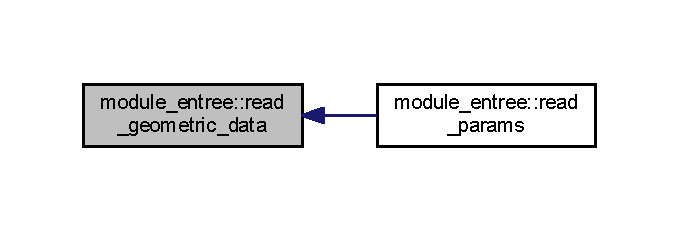
\includegraphics[width=326pt]{namespacemodule__entree_ae5047aaa626b5cac3c9f98267f502669_icgraph}
\end{center}
\end{figure}


\hypertarget{namespacemodule__entree_a4a8eec4484896ca8cb249548e1cf537f}{}\index{module\+\_\+entree@{module\+\_\+entree}!read\+\_\+params@{read\+\_\+params}}
\index{read\+\_\+params@{read\+\_\+params}!module\+\_\+entree@{module\+\_\+entree}}
\subsubsection[{read\+\_\+params}]{\setlength{\rightskip}{0pt plus 5cm}subroutine module\+\_\+entree\+::read\+\_\+params (
\begin{DoxyParamCaption}
\item[{type({\bf type\+\_\+data})}]{data, }
\item[{double precision}]{epsilon, }
\item[{double precision, dimension(\+:), pointer}]{coord\+\_\+min, }
\item[{double precision, dimension(\+:), pointer}]{coord\+\_\+max, }
\item[{integer}]{nb\+\_\+proc, }
\item[{integer, dimension(\+:), pointer}]{partitioning, }
\item[{character (len=30)}]{input\+\_\+file, }
\item[{double precision}]{sigma, }
\item[{integer}]{nb\+\_\+clusters\+\_\+max, }
\item[{integer, dimension(\+:), pointer}]{list\+\_\+nb\+\_\+clusters, }
\item[{type({\bf type\+\_\+clustering\+\_\+param})}]{clust\+\_\+param}
\end{DoxyParamCaption}
)}\label{namespacemodule__entree_a4a8eec4484896ca8cb249548e1cf537f}


Reads a file in which there is the whole information on the data. 


\begin{DoxyParams}[1]{Parameters}
\mbox{\tt in}  & {\em nb\+\_\+proc} & the number of processors used \\
\hline
\mbox{\tt in,out}  & {\em data} & the entire data for computing \\
\hline
\mbox{\tt out}  & {\em input\+\_\+file} & the name of the text file where input data is written \\
\hline
\mbox{\tt out}  & {\em coord\+\_\+max} & the maxima along each dimension of the data (coordinates) \\
\hline
\mbox{\tt out}  & {\em coord\+\_\+min} & the minima along each dimension of the data (coordinates) \\
\hline
\mbox{\tt out}  & {\em epsilon} & the slice thickness \\
\hline
\mbox{\tt out}  & {\em sigma} & the affinity parameter \\
\hline
\mbox{\tt out}  & {\em nb\+\_\+clusters\+\_\+max} & the maximum number of clusters \\
\hline
\mbox{\tt out}  & {\em list\+\_\+nb\+\_\+clusters} & the imposed numbers of clusters list for testing purpose (useless) \\
\hline
\mbox{\tt out}  & {\em partitioning} & the partitionning (number of processors along each dimension) \\
\hline
\end{DoxyParams}


Here is the call graph for this function\+:\nopagebreak
\begin{figure}[H]
\begin{center}
\leavevmode
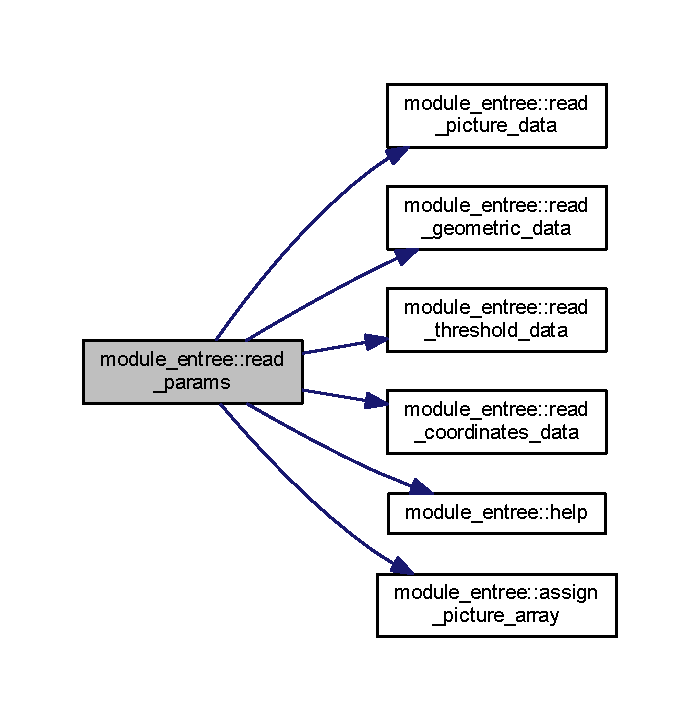
\includegraphics[width=336pt]{namespacemodule__entree_a4a8eec4484896ca8cb249548e1cf537f_cgraph}
\end{center}
\end{figure}


\hypertarget{namespacemodule__entree_aaa0e9ef36218a32292aa65a9b8602cda}{}\index{module\+\_\+entree@{module\+\_\+entree}!read\+\_\+picture\+\_\+data@{read\+\_\+picture\+\_\+data}}
\index{read\+\_\+picture\+\_\+data@{read\+\_\+picture\+\_\+data}!module\+\_\+entree@{module\+\_\+entree}}
\subsubsection[{read\+\_\+picture\+\_\+data}]{\setlength{\rightskip}{0pt plus 5cm}subroutine module\+\_\+entree\+::read\+\_\+picture\+\_\+data (
\begin{DoxyParamCaption}
\item[{character (len=30)}]{input\+\_\+file, }
\item[{type({\bf type\+\_\+data})}]{data, }
\item[{double precision, dimension(\+:), pointer}]{coord\+\_\+min, }
\item[{double precision, dimension(\+:), pointer}]{coord\+\_\+max}
\end{DoxyParamCaption}
)}\label{namespacemodule__entree_aaa0e9ef36218a32292aa65a9b8602cda}


Reads data written in picture format. 

This type of file starts with two {\itshape integers} separated by a blank space\+: the first one corresponds to the dimension of the image and the second one the number of attributes (typically, the attributes could be the color channel intensities). The following line is composed of two {\itshape integers} separated by a blank space\+: the first one corresponds to the number of pixels in a column and the second one to the number of pixels in a row. Then, next lines are composed of {\itshape double} numbers separated by blank spaces. Each of these lines corresponds to the value of the attributes for each pixel. The coordinates of the pixels are implicit as they are ordered by rows. \begin{DoxyNote}{Note}
The attributes are stored in the field \hyperlink{structmodule__structure_1_1type__data_ac7205be3a73581de07ce87c73512e053}{type\+\_\+data\+::coord} and so O\+N\+L\+Y the color will be taken into account. 

The outputs {\itshape coordmax} and {\itshape coordmin} are computed according to the position of the pixels. 
\end{DoxyNote}
\begin{DoxySeeAlso}{See also}
\hyperlink{namespacemodule__entree_a08bc5eb1225bf568c94df30b22f04e03}{assign\+\_\+picture\+\_\+array()}, \hyperlink{namespacemodule__entree_a93d220ea64cd5e1d155255bca188de0c}{read\+\_\+coordinates\+\_\+data()}, \hyperlink{namespacemodule__entree_a25df009403bc610c2ef3b3a151574979}{read\+\_\+threshold\+\_\+data()}, \hyperlink{namespacemodule__entree_ae5047aaa626b5cac3c9f98267f502669}{read\+\_\+geometric\+\_\+data} 
\end{DoxySeeAlso}

\begin{DoxyParams}[1]{Parameters}
\mbox{\tt in}  & {\em input\+\_\+file} & the name of the text file where input data is written \\
\hline
\mbox{\tt in,out}  & {\em data} & the entire data for computing \\
\hline
\mbox{\tt out}  & {\em coord\+\_\+max} & the maxima along each dimension of the data (coordinates) \\
\hline
\mbox{\tt out}  & {\em coord\+\_\+min} & the minima along each dimension of the data (coordinates) \\
\hline
\end{DoxyParams}


Here is the caller graph for this function\+:\nopagebreak
\begin{figure}[H]
\begin{center}
\leavevmode
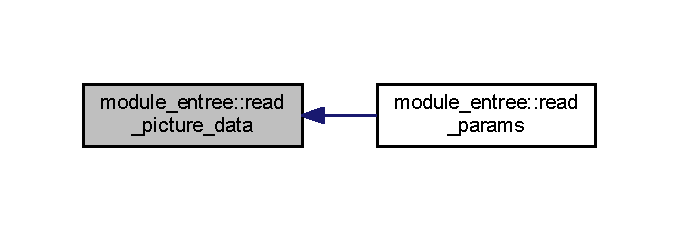
\includegraphics[width=326pt]{namespacemodule__entree_aaa0e9ef36218a32292aa65a9b8602cda_icgraph}
\end{center}
\end{figure}


\hypertarget{namespacemodule__entree_a25df009403bc610c2ef3b3a151574979}{}\index{module\+\_\+entree@{module\+\_\+entree}!read\+\_\+threshold\+\_\+data@{read\+\_\+threshold\+\_\+data}}
\index{read\+\_\+threshold\+\_\+data@{read\+\_\+threshold\+\_\+data}!module\+\_\+entree@{module\+\_\+entree}}
\subsubsection[{read\+\_\+threshold\+\_\+data}]{\setlength{\rightskip}{0pt plus 5cm}subroutine module\+\_\+entree\+::read\+\_\+threshold\+\_\+data (
\begin{DoxyParamCaption}
\item[{character (len=30)}]{input\+\_\+file, }
\item[{type({\bf type\+\_\+data})}]{data, }
\item[{double precision, dimension(\+:), pointer}]{coord\+\_\+min, }
\item[{double precision, dimension(\+:), pointer}]{coord\+\_\+max}
\end{DoxyParamCaption}
)}\label{namespacemodule__entree_a25df009403bc610c2ef3b3a151574979}


Reads data written in threshold format. 

This type of file starts with two {\itshape integers} separated by a blank space\+: the first one corresponds to the dimension of the image and the second one the number of attributes (typically, the attributes could be the color channel intensities). The following line is composed of two {\itshape integers} separated by a blank space\+: the first one corresponds to the number of pixels in a column and the second one to the number of pixels in a row. Then, next lines are composed of {\itshape double} numbers separated by blank spaces. Each of these lines corresponds to the value of the attributes for each pixel. The coordinates of the pixels are implicit as they are ordered by rows. \begin{DoxyNote}{Note}
The attributes are stored in the field \hyperlink{structmodule__structure_1_1type__data_ac7205be3a73581de07ce87c73512e053}{type\+\_\+data\+::coord} and so O\+N\+L\+Y the color will be taken into account 

The outputs {\itshape coordmax} and {\itshape coordmin} are computed according to the color of the pixels. 
\end{DoxyNote}
\begin{DoxySeeAlso}{See also}
\hyperlink{namespacemodule__entree_a08bc5eb1225bf568c94df30b22f04e03}{assign\+\_\+picture\+\_\+array()}, \hyperlink{namespacemodule__entree_aaa0e9ef36218a32292aa65a9b8602cda}{read\+\_\+picture\+\_\+data()}, \hyperlink{namespacemodule__entree_a93d220ea64cd5e1d155255bca188de0c}{read\+\_\+coordinates\+\_\+data()}, \hyperlink{namespacemodule__entree_ae5047aaa626b5cac3c9f98267f502669}{read\+\_\+geometric\+\_\+data} 
\end{DoxySeeAlso}

\begin{DoxyParams}[1]{Parameters}
\mbox{\tt in}  & {\em input\+\_\+file} & the name of the text file where input data is written \\
\hline
\mbox{\tt in,out}  & {\em data} & the entire data for computing \\
\hline
\mbox{\tt out}  & {\em coord\+\_\+max} & the maxima along each dimension of the data (coordinates) \\
\hline
\mbox{\tt out}  & {\em coord\+\_\+min} & the minima along each dimension of the data (coordinates) \\
\hline
\end{DoxyParams}


Here is the caller graph for this function\+:\nopagebreak
\begin{figure}[H]
\begin{center}
\leavevmode
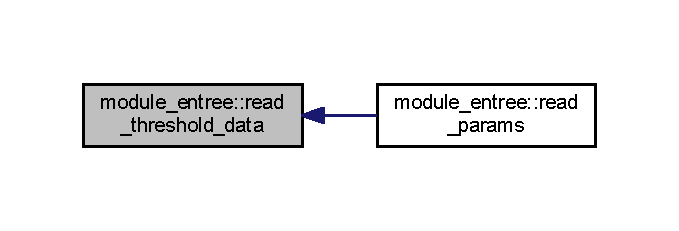
\includegraphics[width=326pt]{namespacemodule__entree_a25df009403bc610c2ef3b3a151574979_icgraph}
\end{center}
\end{figure}



\hypertarget{namespacemodule__mpi}{}\section{module\+\_\+mpi Module Reference}
\label{namespacemodule__mpi}\index{module\+\_\+mpi@{module\+\_\+mpi}}


Contains methods related to parallelism.  


\subsection*{Functions/\+Subroutines}
\begin{DoxyCompactItemize}
\item 
subroutine \hyperlink{namespacemodule__mpi_a8f29a8b24f027344c03e639dc747e849}{send\+\_\+partitioning} (nb\+\_\+proc, data, points\+\_\+by\+\_\+domain, ddat, partitioned\+\_\+data)
\begin{DoxyCompactList}\small\item\em Sends the partitionning. \end{DoxyCompactList}\item 
subroutine \hyperlink{namespacemodule__mpi_a2066496a812a1babe9ad15d90d01feea}{receive\+\_\+partitioning} (proc\+\_\+id, partitioned\+\_\+data)
\begin{DoxyCompactList}\small\item\em Receives the partitionning. \end{DoxyCompactList}\item 
subroutine \hyperlink{namespacemodule__mpi_a62be40b2a3129f7c49677cc68eba40e8}{receive\+\_\+number\+\_\+clusters} (nb\+\_\+proc, nb\+\_\+clusters, points\+\_\+by\+\_\+domain, partitioned\+\_\+data, array\+\_\+clust)
\begin{DoxyCompactList}\small\item\em Receives the number of clusters. \end{DoxyCompactList}\item 
subroutine \hyperlink{namespacemodule__mpi_a5254902c6427631ec28067e9c88481f3}{send\+\_\+number\+\_\+clusters} (proc\+\_\+id, partitioned\+\_\+data)
\begin{DoxyCompactList}\small\item\em Sends the number of clusters. \end{DoxyCompactList}\item 
subroutine \hyperlink{namespacemodule__mpi_a0e866540092c31b9cd5fb527cda5714e}{send\+\_\+clusters} (proc\+\_\+id, partitioned\+\_\+data)
\begin{DoxyCompactList}\small\item\em Sends the clusters. \end{DoxyCompactList}\item 
subroutine \hyperlink{namespacemodule__mpi_ac81a5a711ffecf500db9dd0d05bedd29}{receive\+\_\+clusters} (nb\+\_\+proc, nb\+\_\+clusters, points\+\_\+by\+\_\+domain, ddat, partitioned\+\_\+data, cluster\+\_\+map, array\+\_\+clust, points\+\_\+by\+\_\+cluster)
\begin{DoxyCompactList}\small\item\em Receives the clusters. \end{DoxyCompactList}\end{DoxyCompactItemize}


\subsection{Detailed Description}
Contains methods related to parallelism. 

\subsection{Function/\+Subroutine Documentation}
\hypertarget{namespacemodule__mpi_ac81a5a711ffecf500db9dd0d05bedd29}{}\index{module\+\_\+mpi@{module\+\_\+mpi}!receive\+\_\+clusters@{receive\+\_\+clusters}}
\index{receive\+\_\+clusters@{receive\+\_\+clusters}!module\+\_\+mpi@{module\+\_\+mpi}}
\subsubsection[{receive\+\_\+clusters}]{\setlength{\rightskip}{0pt plus 5cm}subroutine module\+\_\+mpi\+::receive\+\_\+clusters (
\begin{DoxyParamCaption}
\item[{integer}]{nb\+\_\+proc, }
\item[{integer}]{nb\+\_\+clusters, }
\item[{integer, dimension(\+:), pointer}]{points\+\_\+by\+\_\+domain, }
\item[{integer, dimension(\+:,\+:), pointer}]{ddat, }
\item[{type({\bf type\+\_\+data})}]{partitioned\+\_\+data, }
\item[{integer, dimension(\+:,\+:), pointer}]{cluster\+\_\+map, }
\item[{type({\bf type\+\_\+clusters}), dimension(\+:), pointer}]{array\+\_\+clust, }
\item[{integer, dimension(\+:), pointer}]{points\+\_\+by\+\_\+cluster}
\end{DoxyParamCaption}
)}\label{namespacemodule__mpi_ac81a5a711ffecf500db9dd0d05bedd29}


Receives the clusters. 

This method receives the computed clusters in each domain from the slave processes. \begin{DoxyNote}{Note}
It has to be called by the master process. 
\end{DoxyNote}
\begin{DoxySeeAlso}{See also}
\hyperlink{namespacemodule__mpi_a0e866540092c31b9cd5fb527cda5714e}{send\+\_\+clusters()} 
\end{DoxySeeAlso}

\begin{DoxyParams}[1]{Parameters}
\mbox{\tt in}  & {\em array\+\_\+clust} & the number of clusters and elements per cluster computed by each processor \\
\hline
\mbox{\tt in}  & {\em partitioned\+\_\+data} & the partitioned data for computing \\
\hline
\mbox{\tt in}  & {\em assignements} & the assignement of each point in a partition \\
\hline
\mbox{\tt in}  & {\em nb\+\_\+clusters} & the number of clusters \\
\hline
\mbox{\tt in}  & {\em nb\+\_\+clusters} & the number of clusters \\
\hline
\mbox{\tt in}  & {\em nb\+\_\+clusters} & the number of clusters \\
\hline
\mbox{\tt in}  & {\em nb\+\_\+proc} & the number of processors used \\
\hline
\mbox{\tt in}  & {\em points\+\_\+by\+\_\+domain} & the number of points in each partition \\
\hline
\mbox{\tt out}  & {\em cluster\+\_\+map} & the cluster indices and the number of points in each cluster \\
\hline
\mbox{\tt out}  & {\em points\+\_\+by\+\_\+cluster} & the number of points in each cluster \\
\hline
\end{DoxyParams}
\hypertarget{namespacemodule__mpi_a62be40b2a3129f7c49677cc68eba40e8}{}\index{module\+\_\+mpi@{module\+\_\+mpi}!receive\+\_\+number\+\_\+clusters@{receive\+\_\+number\+\_\+clusters}}
\index{receive\+\_\+number\+\_\+clusters@{receive\+\_\+number\+\_\+clusters}!module\+\_\+mpi@{module\+\_\+mpi}}
\subsubsection[{receive\+\_\+number\+\_\+clusters}]{\setlength{\rightskip}{0pt plus 5cm}subroutine module\+\_\+mpi\+::receive\+\_\+number\+\_\+clusters (
\begin{DoxyParamCaption}
\item[{integer}]{nb\+\_\+proc, }
\item[{integer}]{nb\+\_\+clusters, }
\item[{integer, dimension(\+:), pointer}]{points\+\_\+by\+\_\+domain, }
\item[{type({\bf type\+\_\+data})}]{partitioned\+\_\+data, }
\item[{type({\bf type\+\_\+clusters}), dimension(\+:), pointer}]{array\+\_\+clust}
\end{DoxyParamCaption}
)}\label{namespacemodule__mpi_a62be40b2a3129f7c49677cc68eba40e8}


Receives the number of clusters. 

This method receives from the slave processes the number of clusters in each domain and the number of elements in each cluster. \begin{DoxyNote}{Note}
It has to be called by the master process. 
\end{DoxyNote}
\begin{DoxySeeAlso}{See also}
\hyperlink{namespacemodule__mpi_a5254902c6427631ec28067e9c88481f3}{send\+\_\+number\+\_\+clusters()} 
\end{DoxySeeAlso}

\begin{DoxyParams}[1]{Parameters}
\mbox{\tt in}  & {\em partitioned\+\_\+data} & the partitioned data for computing \\
\hline
\mbox{\tt in}  & {\em nb\+\_\+proc} & the number of processors used \\
\hline
\mbox{\tt in}  & {\em points\+\_\+by\+\_\+domain} & the number of points in each partition \\
\hline
\mbox{\tt out}  & {\em array\+\_\+clust} & the number of clusters and elements per cluster computed by each processor \\
\hline
\mbox{\tt out}  & {\em nb\+\_\+clusters} & the number of clusters \\
\hline
\mbox{\tt out}  & {\em nb\+\_\+clusters} & the number of clusters \\
\hline
\mbox{\tt out}  & {\em nb\+\_\+clusters} & the number of clusters \\
\hline
\end{DoxyParams}
\hypertarget{namespacemodule__mpi_a2066496a812a1babe9ad15d90d01feea}{}\index{module\+\_\+mpi@{module\+\_\+mpi}!receive\+\_\+partitioning@{receive\+\_\+partitioning}}
\index{receive\+\_\+partitioning@{receive\+\_\+partitioning}!module\+\_\+mpi@{module\+\_\+mpi}}
\subsubsection[{receive\+\_\+partitioning}]{\setlength{\rightskip}{0pt plus 5cm}subroutine module\+\_\+mpi\+::receive\+\_\+partitioning (
\begin{DoxyParamCaption}
\item[{integer}]{proc\+\_\+id, }
\item[{type({\bf type\+\_\+data})}]{partitioned\+\_\+data}
\end{DoxyParamCaption}
)}\label{namespacemodule__mpi_a2066496a812a1babe9ad15d90d01feea}


Receives the partitionning. 

This method receives from the master process the number of points, the dimension and all the points of the dedicated domain. \begin{DoxyNote}{Note}
It has to be called by a slave process 
\end{DoxyNote}
\begin{DoxySeeAlso}{See also}
\hyperlink{namespacemodule__mpi_a8f29a8b24f027344c03e639dc747e849}{send\+\_\+partitioning()}, \hyperlink{namespacemodule__decoupe_a523f2f851f39859d9c60114c934b2d66}{partition\+\_\+with\+\_\+interface()}, \hyperlink{namespacemodule__decoupe_a6f29dcc8367ffa44fa720260882fa04e}{partition\+\_\+with\+\_\+overlapping()} 
\end{DoxySeeAlso}

\begin{DoxyParams}[1]{Parameters}
\mbox{\tt in}  & {\em proc\+\_\+id} & the processus identifier \\
\hline
\mbox{\tt out}  & {\em partitioned\+\_\+data} & the partitioned data for computing \\
\hline
\end{DoxyParams}
\hypertarget{namespacemodule__mpi_a0e866540092c31b9cd5fb527cda5714e}{}\index{module\+\_\+mpi@{module\+\_\+mpi}!send\+\_\+clusters@{send\+\_\+clusters}}
\index{send\+\_\+clusters@{send\+\_\+clusters}!module\+\_\+mpi@{module\+\_\+mpi}}
\subsubsection[{send\+\_\+clusters}]{\setlength{\rightskip}{0pt plus 5cm}subroutine module\+\_\+mpi\+::send\+\_\+clusters (
\begin{DoxyParamCaption}
\item[{integer}]{proc\+\_\+id, }
\item[{type({\bf type\+\_\+data})}]{partitioned\+\_\+data}
\end{DoxyParamCaption}
)}\label{namespacemodule__mpi_a0e866540092c31b9cd5fb527cda5714e}


Sends the clusters. 

This method sends the computed clusters to the master process. \begin{DoxyNote}{Note}
It has to be called by a slave process. 
\end{DoxyNote}
\begin{DoxySeeAlso}{See also}
\hyperlink{namespacemodule__mpi_ac81a5a711ffecf500db9dd0d05bedd29}{receive\+\_\+clusters()} 
\end{DoxySeeAlso}

\begin{DoxyParams}[1]{Parameters}
\mbox{\tt in}  & {\em partitioned\+\_\+data} & the partitioned data for computing \\
\hline
\mbox{\tt in}  & {\em proc\+\_\+id} & the processus identifier \\
\hline
\end{DoxyParams}
\hypertarget{namespacemodule__mpi_a5254902c6427631ec28067e9c88481f3}{}\index{module\+\_\+mpi@{module\+\_\+mpi}!send\+\_\+number\+\_\+clusters@{send\+\_\+number\+\_\+clusters}}
\index{send\+\_\+number\+\_\+clusters@{send\+\_\+number\+\_\+clusters}!module\+\_\+mpi@{module\+\_\+mpi}}
\subsubsection[{send\+\_\+number\+\_\+clusters}]{\setlength{\rightskip}{0pt plus 5cm}subroutine module\+\_\+mpi\+::send\+\_\+number\+\_\+clusters (
\begin{DoxyParamCaption}
\item[{integer}]{proc\+\_\+id, }
\item[{type({\bf type\+\_\+data})}]{partitioned\+\_\+data}
\end{DoxyParamCaption}
)}\label{namespacemodule__mpi_a5254902c6427631ec28067e9c88481f3}


Sends the number of clusters. 

This method sends to the master process the number of clusters and the number of elements in each cluster. \begin{DoxyNote}{Note}
It has to be called by a slave process. 
\end{DoxyNote}
\begin{DoxySeeAlso}{See also}
\hyperlink{namespacemodule__mpi_a62be40b2a3129f7c49677cc68eba40e8}{receive\+\_\+number\+\_\+clusters()} 
\end{DoxySeeAlso}

\begin{DoxyParams}[1]{Parameters}
\mbox{\tt in}  & {\em partitioned\+\_\+data} & the partitioned data for computing \\
\hline
\mbox{\tt in}  & {\em proc\+\_\+id} & the processus identifier \\
\hline
\end{DoxyParams}
\hypertarget{namespacemodule__mpi_a8f29a8b24f027344c03e639dc747e849}{}\index{module\+\_\+mpi@{module\+\_\+mpi}!send\+\_\+partitioning@{send\+\_\+partitioning}}
\index{send\+\_\+partitioning@{send\+\_\+partitioning}!module\+\_\+mpi@{module\+\_\+mpi}}
\subsubsection[{send\+\_\+partitioning}]{\setlength{\rightskip}{0pt plus 5cm}subroutine module\+\_\+mpi\+::send\+\_\+partitioning (
\begin{DoxyParamCaption}
\item[{integer}]{nb\+\_\+proc, }
\item[{type({\bf type\+\_\+data})}]{data, }
\item[{integer, dimension(\+:), pointer}]{points\+\_\+by\+\_\+domain, }
\item[{integer, dimension(\+:,\+:), pointer}]{ddat, }
\item[{type({\bf type\+\_\+data})}]{partitioned\+\_\+data}
\end{DoxyParamCaption}
)}\label{namespacemodule__mpi_a8f29a8b24f027344c03e639dc747e849}


Sends the partitionning. 

This method sends to each slave process the number of points, the dimension and all the points of the dedicated domain. Then, it creates \begin{DoxyNote}{Note}
It has to be called by the master process 
\end{DoxyNote}
\begin{DoxySeeAlso}{See also}
\hyperlink{namespacemodule__mpi_a2066496a812a1babe9ad15d90d01feea}{receive\+\_\+partitioning()}, \hyperlink{namespacemodule__decoupe_a523f2f851f39859d9c60114c934b2d66}{partition\+\_\+with\+\_\+interface()}, \hyperlink{namespacemodule__decoupe_a6f29dcc8367ffa44fa720260882fa04e}{partition\+\_\+with\+\_\+overlapping()} 
\end{DoxySeeAlso}

\begin{DoxyParams}[1]{Parameters}
\mbox{\tt in}  & {\em assignements} & the assignement of each point in a partition \\
\hline
\mbox{\tt in}  & {\em nb\+\_\+proc} & the number of processors used \\
\hline
\mbox{\tt in}  & {\em points\+\_\+by\+\_\+domain} & the number of points in each partition \\
\hline
\mbox{\tt in,out}  & {\em data} & the entire data for computing \\
\hline
\mbox{\tt out}  & {\em partitioned\+\_\+data} & the partitioned data for computing \\
\hline
\end{DoxyParams}

\hypertarget{namespacemodule__solve}{}\section{module\+\_\+solve Module Reference}
\label{namespacemodule__solve}\index{module\+\_\+solve@{module\+\_\+solve}}


Contains methods from Lapack library dealing with eigen values computing.  


\subsection*{Functions/\+Subroutines}
\begin{DoxyCompactItemize}
\item 
subroutine \hyperlink{namespacemodule__solve_a6e1a9cb766d06da8f5ac09592d460849}{solve\+\_\+dgeevx} (N, A, V\+R, W\+R)
\item 
subroutine \hyperlink{namespacemodule__solve_a2a2b6bf2dc5b4e3d08908fa43fca207b}{solve\+\_\+dgeev} (N, A, V\+R, W\+R)
\item 
subroutine \hyperlink{namespacemodule__solve_a52e46b41df1e4cf29e5ae9e908ed4293}{solve\+\_\+dsyev} (N, A, W, L\+W\+O\+R\+K)
\item 
subroutine \hyperlink{namespacemodule__solve_a71d616a8ea24efa60b9d9227d0a40309}{solve\+\_\+dsyevr} (k, N, A, Z, L\+W\+O\+R\+K, L\+I\+W\+O\+R\+K, W, M)
\item 
subroutine \hyperlink{namespacemodule__solve_af9f9bed9d344018397cbc722f70a6bb0}{solve\+\_\+dsyevx} (k, N, A, Z, L\+W\+O\+R\+K, L\+I\+W\+O\+R\+K, W, M)
\end{DoxyCompactItemize}


\subsection{Detailed Description}
Contains methods from Lapack library dealing with eigen values computing. 

\subsection{Function/\+Subroutine Documentation}
\hypertarget{namespacemodule__solve_a2a2b6bf2dc5b4e3d08908fa43fca207b}{}\index{module\+\_\+solve@{module\+\_\+solve}!solve\+\_\+dgeev@{solve\+\_\+dgeev}}
\index{solve\+\_\+dgeev@{solve\+\_\+dgeev}!module\+\_\+solve@{module\+\_\+solve}}
\subsubsection[{solve\+\_\+dgeev}]{\setlength{\rightskip}{0pt plus 5cm}subroutine module\+\_\+solve\+::solve\+\_\+dgeev (
\begin{DoxyParamCaption}
\item[{integer}]{N, }
\item[{double precision, dimension(\+:,\+:), pointer}]{A, }
\item[{double precision, dimension(\+:,\+:), pointer}]{V\+R, }
\item[{double precision, dimension(\+:), pointer}]{W\+R}
\end{DoxyParamCaption}
)}\label{namespacemodule__solve_a2a2b6bf2dc5b4e3d08908fa43fca207b}

\begin{DoxyParams}[1]{Parameters}
\mbox{\tt in}  & {\em A} & the affinity matrix \\
\hline
\mbox{\tt in}  & {\em N} & \\
\hline
\mbox{\tt out}  & {\em V\+R} & \\
\hline
\mbox{\tt out}  & {\em W\+R} & \\
\hline
\end{DoxyParams}


Here is the caller graph for this function\+:\nopagebreak
\begin{figure}[H]
\begin{center}
\leavevmode
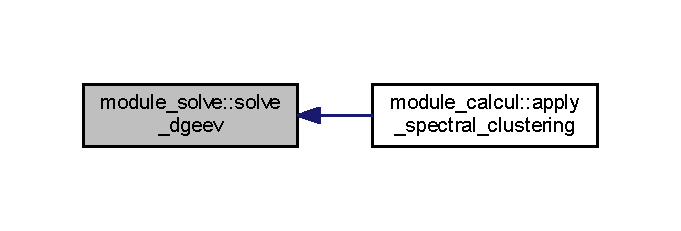
\includegraphics[width=327pt]{namespacemodule__solve_a2a2b6bf2dc5b4e3d08908fa43fca207b_icgraph}
\end{center}
\end{figure}


\hypertarget{namespacemodule__solve_a6e1a9cb766d06da8f5ac09592d460849}{}\index{module\+\_\+solve@{module\+\_\+solve}!solve\+\_\+dgeevx@{solve\+\_\+dgeevx}}
\index{solve\+\_\+dgeevx@{solve\+\_\+dgeevx}!module\+\_\+solve@{module\+\_\+solve}}
\subsubsection[{solve\+\_\+dgeevx}]{\setlength{\rightskip}{0pt plus 5cm}subroutine module\+\_\+solve\+::solve\+\_\+dgeevx (
\begin{DoxyParamCaption}
\item[{integer}]{N, }
\item[{double precision, dimension(\+:,\+:), pointer}]{A, }
\item[{double precision, dimension(\+:,\+:), pointer}]{V\+R, }
\item[{double precision, dimension(\+:), pointer}]{W\+R}
\end{DoxyParamCaption}
)}\label{namespacemodule__solve_a6e1a9cb766d06da8f5ac09592d460849}

\begin{DoxyParams}{Parameters}
{\em A} & the affinity matrix \\
\hline
{\em V\+R} & \\
\hline
{\em W\+R} & \\
\hline
{\em N} & \\
\hline
\end{DoxyParams}
\hypertarget{namespacemodule__solve_a52e46b41df1e4cf29e5ae9e908ed4293}{}\index{module\+\_\+solve@{module\+\_\+solve}!solve\+\_\+dsyev@{solve\+\_\+dsyev}}
\index{solve\+\_\+dsyev@{solve\+\_\+dsyev}!module\+\_\+solve@{module\+\_\+solve}}
\subsubsection[{solve\+\_\+dsyev}]{\setlength{\rightskip}{0pt plus 5cm}subroutine module\+\_\+solve\+::solve\+\_\+dsyev (
\begin{DoxyParamCaption}
\item[{integer}]{N, }
\item[{double precision, dimension(n,n)}]{A, }
\item[{double precision, dimension(n)}]{W, }
\item[{integer}]{L\+W\+O\+R\+K}
\end{DoxyParamCaption}
)}\label{namespacemodule__solve_a52e46b41df1e4cf29e5ae9e908ed4293}

\begin{DoxyParams}{Parameters}
{\em A} & the affinity matrix \\
\hline
{\em W} & \\
\hline
{\em L\+W\+O\+R\+K} & \\
\hline
{\em N} & \\
\hline
\end{DoxyParams}
\hypertarget{namespacemodule__solve_a71d616a8ea24efa60b9d9227d0a40309}{}\index{module\+\_\+solve@{module\+\_\+solve}!solve\+\_\+dsyevr@{solve\+\_\+dsyevr}}
\index{solve\+\_\+dsyevr@{solve\+\_\+dsyevr}!module\+\_\+solve@{module\+\_\+solve}}
\subsubsection[{solve\+\_\+dsyevr}]{\setlength{\rightskip}{0pt plus 5cm}subroutine module\+\_\+solve\+::solve\+\_\+dsyevr (
\begin{DoxyParamCaption}
\item[{integer}]{k, }
\item[{integer}]{N, }
\item[{double precision, dimension(n,n)}]{A, }
\item[{double precision, dimension(n,n)}]{Z, }
\item[{integer}]{L\+W\+O\+R\+K, }
\item[{integer}]{L\+I\+W\+O\+R\+K, }
\item[{double precision, dimension(n)}]{W, }
\item[{integer}]{M}
\end{DoxyParamCaption}
)}\label{namespacemodule__solve_a71d616a8ea24efa60b9d9227d0a40309}

\begin{DoxyParams}{Parameters}
{\em A} & the affinity matrix \\
\hline
{\em Z} & the matrix of eigen vectors \\
\hline
{\em W} & \\
\hline
{\em k} & \\
\hline
{\em L\+I\+W\+O\+R\+K} & \\
\hline
{\em L\+W\+O\+R\+K} & \\
\hline
{\em M} & \\
\hline
{\em N} & \\
\hline
\end{DoxyParams}
\hypertarget{namespacemodule__solve_af9f9bed9d344018397cbc722f70a6bb0}{}\index{module\+\_\+solve@{module\+\_\+solve}!solve\+\_\+dsyevx@{solve\+\_\+dsyevx}}
\index{solve\+\_\+dsyevx@{solve\+\_\+dsyevx}!module\+\_\+solve@{module\+\_\+solve}}
\subsubsection[{solve\+\_\+dsyevx}]{\setlength{\rightskip}{0pt plus 5cm}subroutine module\+\_\+solve\+::solve\+\_\+dsyevx (
\begin{DoxyParamCaption}
\item[{integer}]{k, }
\item[{integer}]{N, }
\item[{double precision, dimension(n,n)}]{A, }
\item[{double precision, dimension(n,n)}]{Z, }
\item[{integer}]{L\+W\+O\+R\+K, }
\item[{integer}]{L\+I\+W\+O\+R\+K, }
\item[{double precision, dimension(n)}]{W, }
\item[{integer}]{M}
\end{DoxyParamCaption}
)}\label{namespacemodule__solve_af9f9bed9d344018397cbc722f70a6bb0}

\begin{DoxyParams}{Parameters}
{\em A} & the affinity matrix \\
\hline
{\em Z} & the matrix of eigen vectors \\
\hline
{\em W} & \\
\hline
{\em k} & \\
\hline
{\em L\+I\+W\+O\+R\+K} & \\
\hline
{\em L\+W\+O\+R\+K} & \\
\hline
{\em M} & \\
\hline
{\em N} & \\
\hline
\end{DoxyParams}

\hypertarget{namespacemodule__sortie}{}\section{module\+\_\+sortie Module Reference}
\label{namespacemodule__sortie}\index{module\+\_\+sortie@{module\+\_\+sortie}}


Contains methods enabling writing results in specific formatted files.  


\subsection*{Functions/\+Subroutines}
\begin{DoxyCompactItemize}
\item 
subroutine \hyperlink{namespacemodule__sortie_a835f7338c29161d6893c6bbddf4174f4}{write\+\_\+domains} (data, nb\+\_\+proc, domains)
\begin{DoxyCompactList}\small\item\em Writes the file containing the domain definitions. \end{DoxyCompactList}\item 
subroutine \hyperlink{namespacemodule__sortie_abd1cdf529e5c71b3186c8d980e3d5117}{write\+\_\+partitioning} (nb\+\_\+proc, data, points\+\_\+by\+\_\+domain, assignements)
\begin{DoxyCompactList}\small\item\em Writes the files containing the partitionning. \end{DoxyCompactList}\item 
subroutine \hyperlink{namespacemodule__sortie_a24e663b5fc236eee7c6fe434493e342e}{write\+\_\+partial\+\_\+clusters} (proc\+\_\+id, partitioned\+\_\+data)
\begin{DoxyCompactList}\small\item\em Writes the file containing the clusters computed by the process. \end{DoxyCompactList}\item 
subroutine \hyperlink{namespacemodule__sortie_a819ceed76e9600e8eec63a7b730d1d92}{write\+\_\+final\+\_\+clusters} (nb\+\_\+clusters, points\+\_\+by\+\_\+cluster, cluster\+\_\+map)
\begin{DoxyCompactList}\small\item\em Writes the files containing the final clusters after grouping. \end{DoxyCompactList}\item 
subroutine \hyperlink{namespacemodule__sortie_a3093c50035046621188d9a0da3b8a587}{write\+\_\+metadata} (mesh, data, nb\+\_\+proc, nb\+\_\+clusters)
\begin{DoxyCompactList}\small\item\em Writes a file containing various information. \end{DoxyCompactList}\end{DoxyCompactItemize}


\subsection{Detailed Description}
Contains methods enabling writing results in specific formatted files. 

\subsection{Function/\+Subroutine Documentation}
\hypertarget{namespacemodule__sortie_a835f7338c29161d6893c6bbddf4174f4}{}\index{module\+\_\+sortie@{module\+\_\+sortie}!write\+\_\+domains@{write\+\_\+domains}}
\index{write\+\_\+domains@{write\+\_\+domains}!module\+\_\+sortie@{module\+\_\+sortie}}
\subsubsection[{write\+\_\+domains}]{\setlength{\rightskip}{0pt plus 5cm}subroutine module\+\_\+sortie\+::write\+\_\+domains (
\begin{DoxyParamCaption}
\item[{type({\bf type\+\_\+data})}]{data, }
\item[{integer}]{nb\+\_\+proc, }
\item[{double precision, dimension(\+:,\+:,\+:), pointer}]{domains}
\end{DoxyParamCaption}
)}\label{namespacemodule__sortie_a835f7338c29161d6893c6bbddf4174f4}


Writes the file containing the domain definitions. 

This methods writes the domain definitions using the following formatting\+: each line contains the two point coordinates of a bound separated by the character \char`\"{}$\vert$\char`\"{}. \begin{DoxyNote}{Note}
The written file is {\itshape fort.\+2}.S 
\end{DoxyNote}

\begin{DoxyParams}[1]{Parameters}
\mbox{\tt in}  & {\em data} & the entire data for computing \\
\hline
\mbox{\tt in}  & {\em domains} & the domains constructed from the bounds \\
\hline
\mbox{\tt in}  & {\em nb\+\_\+proc} & the number of processors used \\
\hline
\end{DoxyParams}


Here is the caller graph for this function\+:\nopagebreak
\begin{figure}[H]
\begin{center}
\leavevmode
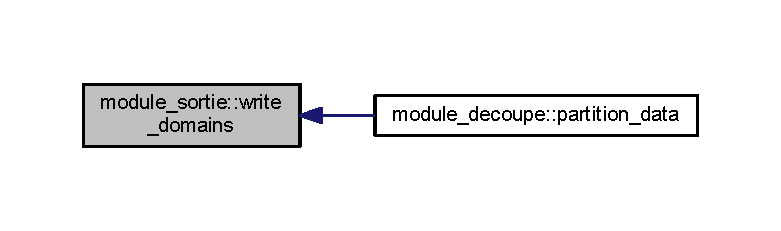
\includegraphics[width=350pt]{namespacemodule__sortie_a835f7338c29161d6893c6bbddf4174f4_icgraph}
\end{center}
\end{figure}


\hypertarget{namespacemodule__sortie_a819ceed76e9600e8eec63a7b730d1d92}{}\index{module\+\_\+sortie@{module\+\_\+sortie}!write\+\_\+final\+\_\+clusters@{write\+\_\+final\+\_\+clusters}}
\index{write\+\_\+final\+\_\+clusters@{write\+\_\+final\+\_\+clusters}!module\+\_\+sortie@{module\+\_\+sortie}}
\subsubsection[{write\+\_\+final\+\_\+clusters}]{\setlength{\rightskip}{0pt plus 5cm}subroutine module\+\_\+sortie\+::write\+\_\+final\+\_\+clusters (
\begin{DoxyParamCaption}
\item[{integer}]{nb\+\_\+clusters, }
\item[{integer, dimension(\+:), pointer}]{points\+\_\+by\+\_\+cluster, }
\item[{integer, dimension(\+:,\+:), pointer}]{cluster\+\_\+map}
\end{DoxyParamCaption}
)}\label{namespacemodule__sortie_a819ceed76e9600e8eec63a7b730d1d92}


Writes the files containing the final clusters after grouping. 

Each file correspond to a cluster. The first number is the number of points in the cluster. Then all the following numbers are the indices of the points that belongs to the cluster. \begin{DoxyNote}{Note}
The written files are {\itshape cluster.\+final.\+x} with x the ids of the clusters. 
\end{DoxyNote}

\begin{DoxyParams}[1]{Parameters}
\mbox{\tt in}  & {\em cluster\+\_\+map} & the cluster indices and the number of points in each cluster \\
\hline
\mbox{\tt in}  & {\em points\+\_\+by\+\_\+cluster} & the number of points in each cluster \\
\hline
\mbox{\tt in,out}  & {\em nb\+\_\+clusters} & the number of clusters \\
\hline
\mbox{\tt in,out}  & {\em nb\+\_\+clusters} & the number of clusters \\
\hline
\mbox{\tt in,out}  & {\em nb\+\_\+clusters} & the number of clusters \\
\hline
\end{DoxyParams}
\hypertarget{namespacemodule__sortie_a3093c50035046621188d9a0da3b8a587}{}\index{module\+\_\+sortie@{module\+\_\+sortie}!write\+\_\+metadata@{write\+\_\+metadata}}
\index{write\+\_\+metadata@{write\+\_\+metadata}!module\+\_\+sortie@{module\+\_\+sortie}}
\subsubsection[{write\+\_\+metadata}]{\setlength{\rightskip}{0pt plus 5cm}subroutine module\+\_\+sortie\+::write\+\_\+metadata (
\begin{DoxyParamCaption}
\item[{character (len=30)}]{mesh, }
\item[{type({\bf type\+\_\+data})}]{data, }
\item[{integer}]{nb\+\_\+proc, }
\item[{integer}]{nb\+\_\+clusters}
\end{DoxyParamCaption}
)}\label{namespacemodule__sortie_a3093c50035046621188d9a0da3b8a587}


Writes a file containing various information. 

The following information is written in {\itshape fort.\+3} file \+: 
\begin{DoxyEnumerate}
\item The data file name  
\item The number of the points in the entire data set  
\item The number of processes used  
\item The partitioning mode (by interface or overlapping)  
\item The number of clusters found  
\item The data file format  
\end{DoxyEnumerate}In the case of a picture format\+: this extra information is written \+: 
\begin{DoxyEnumerate}
\item The image dimension  
\item The image partitioning  
\item The number of attributes  
\item The number of steps (only in geometric format)  
\end{DoxyEnumerate}\begin{DoxySeeAlso}{See also}
\hyperlink{namespacemodule__visuclusters_ab68939a34024c66e1e7cc64a0dcf8736}{read\+\_\+metadata()} 
\end{DoxySeeAlso}

\begin{DoxyParams}[1]{Parameters}
\mbox{\tt in}  & {\em data} & the entire data for computing \\
\hline
\mbox{\tt in}  & {\em input\+\_\+file} & the name of the text file where input data is written \\
\hline
\mbox{\tt in}  & {\em nb\+\_\+clusters} & the number of clusters \\
\hline
\mbox{\tt in}  & {\em nb\+\_\+clusters} & the number of clusters \\
\hline
\mbox{\tt in}  & {\em nb\+\_\+clusters} & the number of clusters \\
\hline
\mbox{\tt in}  & {\em nb\+\_\+proc} & the number of processors used \\
\hline
\end{DoxyParams}
\hypertarget{namespacemodule__sortie_a24e663b5fc236eee7c6fe434493e342e}{}\index{module\+\_\+sortie@{module\+\_\+sortie}!write\+\_\+partial\+\_\+clusters@{write\+\_\+partial\+\_\+clusters}}
\index{write\+\_\+partial\+\_\+clusters@{write\+\_\+partial\+\_\+clusters}!module\+\_\+sortie@{module\+\_\+sortie}}
\subsubsection[{write\+\_\+partial\+\_\+clusters}]{\setlength{\rightskip}{0pt plus 5cm}subroutine module\+\_\+sortie\+::write\+\_\+partial\+\_\+clusters (
\begin{DoxyParamCaption}
\item[{integer}]{proc\+\_\+id, }
\item[{type({\bf type\+\_\+data})}]{partitioned\+\_\+data}
\end{DoxyParamCaption}
)}\label{namespacemodule__sortie_a24e663b5fc236eee7c6fe434493e342e}


Writes the file containing the clusters computed by the process. 

The file starts with the number of points in the domain and the number of dimensions separated by a blank space. The following lines are \+: 
\begin{DoxyItemize}
\item {\bfseries  For coordinates format } \+: the coordinates of a point and the id of the cluster which it belongs to separated by a comma  
\item {\bfseries  For picture formats } \+: the id of the point and the id of the cluster which it belongs to separated by a comma 
\end{DoxyItemize}\begin{DoxyNote}{Note}
The written file is {\itshape cluster.\+partiel.\+x} with x the id of the process 
\end{DoxyNote}

\begin{DoxyParams}[1]{Parameters}
\mbox{\tt in}  & {\em partitioned\+\_\+data} & the partitioned data for computing \\
\hline
\mbox{\tt in}  & {\em proc\+\_\+id} & the processus identifier \\
\hline
\end{DoxyParams}
\hypertarget{namespacemodule__sortie_abd1cdf529e5c71b3186c8d980e3d5117}{}\index{module\+\_\+sortie@{module\+\_\+sortie}!write\+\_\+partitioning@{write\+\_\+partitioning}}
\index{write\+\_\+partitioning@{write\+\_\+partitioning}!module\+\_\+sortie@{module\+\_\+sortie}}
\subsubsection[{write\+\_\+partitioning}]{\setlength{\rightskip}{0pt plus 5cm}subroutine module\+\_\+sortie\+::write\+\_\+partitioning (
\begin{DoxyParamCaption}
\item[{integer}]{nb\+\_\+proc, }
\item[{type({\bf type\+\_\+data})}]{data, }
\item[{integer, dimension(\+:), pointer}]{points\+\_\+by\+\_\+domain, }
\item[{integer, dimension(\+:,\+:), pointer}]{assignements}
\end{DoxyParamCaption}
)}\label{namespacemodule__sortie_abd1cdf529e5c71b3186c8d980e3d5117}


Writes the files containing the partitionning. 

Each file correspond to a domain. The first number is the number of points in the domain. Then the following lines are simply the coordinates of the points (in case of coordinates format) or the color of the pixels (in case of picture format) separated by blank spaces. \begin{DoxyNote}{Note}
The written files are {\itshape decoupe.\+x} with x the ids of the processes. 
\end{DoxyNote}

\begin{DoxyParams}[1]{Parameters}
\mbox{\tt in}  & {\em data} & the entire data for computing \\
\hline
\mbox{\tt in}  & {\em assignements} & the assignement of each point in a partition \\
\hline
\mbox{\tt in}  & {\em nb\+\_\+proc} & the number of processors used \\
\hline
\mbox{\tt in}  & {\em points\+\_\+by\+\_\+domain} & the number of points in each partition \\
\hline
\end{DoxyParams}


Here is the caller graph for this function\+:\nopagebreak
\begin{figure}[H]
\begin{center}
\leavevmode
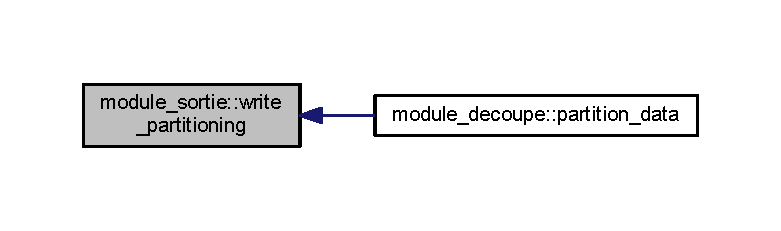
\includegraphics[width=350pt]{namespacemodule__sortie_abd1cdf529e5c71b3186c8d980e3d5117_icgraph}
\end{center}
\end{figure}



\hypertarget{namespacemodule__sparse}{}\section{module\+\_\+sparse Module Reference}
\label{namespacemodule__sparse}\index{module\+\_\+sparse@{module\+\_\+sparse}}
\subsection*{Functions/\+Subroutines}
\begin{DoxyCompactItemize}
\item 
subroutine \hyperlink{namespacemodule__sparse_ac7a222921bd378c5d9d8d41fa05423ad}{apply\+\_\+spectral\+\_\+clustering\+\_\+sparse} (proc\+\_\+id, nb\+\_\+clusters\+\_\+max, nb\+\_\+clusters\+\_\+opt, partitioned\+\_\+data, sigma)
\begin{DoxyCompactList}\small\item\em Computes the clusters using spectral clustering algorithm using sparsity. \end{DoxyCompactList}\item 
subroutine \hyperlink{namespacemodule__sparse_a6fc2f45f94f4ea124ea27f88b8823274}{apply\+\_\+spectral\+\_\+embedding\+\_\+sparse} (nb\+\_\+clusters, n, Z, nnz, A\+S, I\+A\+S, J\+A\+S, ratio, clusters, clusters\+\_\+centers, points\+\_\+by\+\_\+clusters, clusters\+\_\+energies, nb\+\_\+info, proc\+\_\+id, ratio\+\_\+moy, ratio\+\_\+rij, ratio\+\_\+rii)
\begin{DoxyCompactList}\small\item\em Computes the ideal number of clusters using sparsity. \end{DoxyCompactList}\item 
subroutine \hyperlink{namespacemodule__sparse_a172821d54ec6f3bec6f07ca4f9d96d37}{compute\+\_\+matvec\+\_\+prod} (A, I\+A, J\+A, X, Y, n, nnz)
\begin{DoxyCompactList}\small\item\em Computes the matrix vector product using sparsity. \end{DoxyCompactList}\item 
subroutine \hyperlink{namespacemodule__sparse_a1945ecdb844a637fd6372b3686b4df40}{solve\+\_\+arpack} (A, I\+A, J\+A, dim, nnz, nb\+\_\+clusters\+\_\+max, W, Z)
\end{DoxyCompactItemize}


\subsection{Function/\+Subroutine Documentation}
\hypertarget{namespacemodule__sparse_ac7a222921bd378c5d9d8d41fa05423ad}{}\index{module\+\_\+sparse@{module\+\_\+sparse}!apply\+\_\+spectral\+\_\+clustering\+\_\+sparse@{apply\+\_\+spectral\+\_\+clustering\+\_\+sparse}}
\index{apply\+\_\+spectral\+\_\+clustering\+\_\+sparse@{apply\+\_\+spectral\+\_\+clustering\+\_\+sparse}!module\+\_\+sparse@{module\+\_\+sparse}}
\subsubsection[{apply\+\_\+spectral\+\_\+clustering\+\_\+sparse}]{\setlength{\rightskip}{0pt plus 5cm}subroutine module\+\_\+sparse\+::apply\+\_\+spectral\+\_\+clustering\+\_\+sparse (
\begin{DoxyParamCaption}
\item[{integer}]{proc\+\_\+id, }
\item[{integer}]{nb\+\_\+clusters\+\_\+max, }
\item[{integer}]{nb\+\_\+clusters\+\_\+opt, }
\item[{type({\bf type\+\_\+data})}]{partitioned\+\_\+data, }
\item[{double precision}]{sigma}
\end{DoxyParamCaption}
)}\label{namespacemodule__sparse_ac7a222921bd378c5d9d8d41fa05423ad}


Computes the clusters using spectral clustering algorithm using sparsity. 

\begin{DoxySeeAlso}{See also}
\hyperlink{namespacemodule__calcul_a7bf1a318c636b4e204f267103d00114a}{apply\+\_\+spectral\+\_\+clustering()} 
\end{DoxySeeAlso}

\begin{DoxyParams}[1]{Parameters}
\mbox{\tt in}  & {\em sigma} & the affinity parameter \\
\hline
\mbox{\tt in}  & {\em nb\+\_\+clusters\+\_\+max} & the maximum number of clusters \\
\hline
\mbox{\tt in}  & {\em nb\+\_\+clusters\+\_\+opt} & the optimal number of clusters \\
\hline
\mbox{\tt in}  & {\em proc\+\_\+id} & the processus identifier \\
\hline
\mbox{\tt in,out}  & {\em partitioned\+\_\+data} & the partitioned data for computing \\
\hline
\end{DoxyParams}


Here is the call graph for this function\+:\nopagebreak
\begin{figure}[H]
\begin{center}
\leavevmode
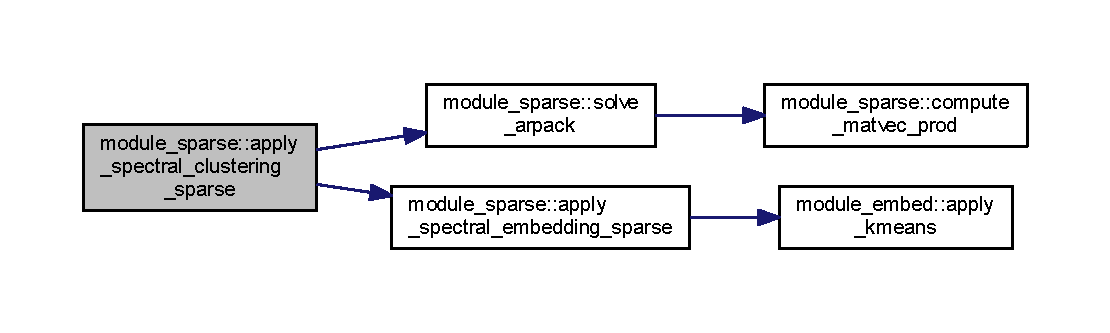
\includegraphics[width=350pt]{namespacemodule__sparse_ac7a222921bd378c5d9d8d41fa05423ad_cgraph}
\end{center}
\end{figure}


\hypertarget{namespacemodule__sparse_a6fc2f45f94f4ea124ea27f88b8823274}{}\index{module\+\_\+sparse@{module\+\_\+sparse}!apply\+\_\+spectral\+\_\+embedding\+\_\+sparse@{apply\+\_\+spectral\+\_\+embedding\+\_\+sparse}}
\index{apply\+\_\+spectral\+\_\+embedding\+\_\+sparse@{apply\+\_\+spectral\+\_\+embedding\+\_\+sparse}!module\+\_\+sparse@{module\+\_\+sparse}}
\subsubsection[{apply\+\_\+spectral\+\_\+embedding\+\_\+sparse}]{\setlength{\rightskip}{0pt plus 5cm}subroutine module\+\_\+sparse\+::apply\+\_\+spectral\+\_\+embedding\+\_\+sparse (
\begin{DoxyParamCaption}
\item[{integer}]{nb\+\_\+clusters, }
\item[{integer}]{n, }
\item[{double precision, dimension(\+:,\+:), pointer}]{Z, }
\item[{integer}]{nnz, }
\item[{double precision, dimension(\+:), pointer}]{A\+S, }
\item[{integer, dimension(\+:), pointer}]{I\+A\+S, }
\item[{integer, dimension(\+:), pointer}]{J\+A\+S, }
\item[{double precision}]{ratio, }
\item[{integer, dimension(\+:), pointer}]{clusters, }
\item[{double precision, dimension(\+:,\+:), pointer}]{clusters\+\_\+centers, }
\item[{integer, dimension(\+:), pointer}]{points\+\_\+by\+\_\+clusters, }
\item[{double precision, dimension(\+:), pointer}]{clusters\+\_\+energies, }
\item[{integer}]{nb\+\_\+info, }
\item[{integer}]{proc\+\_\+id, }
\item[{double precision}]{ratio\+\_\+moy, }
\item[{double precision}]{ratio\+\_\+rij, }
\item[{double precision}]{ratio\+\_\+rii}
\end{DoxyParamCaption}
)}\label{namespacemodule__sparse_a6fc2f45f94f4ea124ea27f88b8823274}


Computes the ideal number of clusters using sparsity. 

\begin{DoxySeeAlso}{See also}
\hyperlink{namespacemodule__embed_ab78350f96b04d0ce2ca0bd10abd50440}{apply\+\_\+spectral\+\_\+embedding()} 
\end{DoxySeeAlso}

\begin{DoxyParams}[1]{Parameters}
\mbox{\tt in}  & {\em Z} & the matrix of eigen vectors \\
\hline
\mbox{\tt in}  & {\em A\+S} & the affinity sparse matrix \\
\hline
\mbox{\tt in}  & {\em n} & \\
\hline
\mbox{\tt in}  & {\em nb\+\_\+clusters} & the number of clusters \\
\hline
\mbox{\tt in}  & {\em nb\+\_\+clusters} & the number of clusters \\
\hline
\mbox{\tt in}  & {\em nb\+\_\+clusters} & the number of clusters \\
\hline
\mbox{\tt in}  & {\em nnz} & the number of non-\/zero coefficients \\
\hline
\mbox{\tt in}  & {\em proc\+\_\+id} & the processus identifier \\
\hline
\mbox{\tt in}  & {\em I\+A\+S} & the row indices of the affinity matrix coefficients \\
\hline
\mbox{\tt in}  & {\em J\+A\+S} & the column indices of the affinity matrix coefficients \\
\hline
\mbox{\tt out}  & {\em clusters\+\_\+centers} & the cluster centers \\
\hline
\mbox{\tt out}  & {\em clusters\+\_\+energies} & the cluster energies \\
\hline
\mbox{\tt out}  & {\em ratio} & the sum of the ratios between Frobenius norm of the off-\/diagonal and the diagonal blocks of the normalized affinity matrix \\
\hline
\mbox{\tt out}  & {\em ratio\+\_\+moy} & \\
\hline
\mbox{\tt out}  & {\em ratio\+\_\+rii} & the sum of the denominator of each ratio \\
\hline
\mbox{\tt out}  & {\em ratio\+\_\+rij} & the sum of the numerators of each ratio \\
\hline
\mbox{\tt out}  & {\em nb\+\_\+info} & the reduced number of clusters (?) \\
\hline
\mbox{\tt out}  & {\em clusters} & indicates which cluster each point belongs to \\
\hline
\mbox{\tt out}  & {\em points\+\_\+by\+\_\+clusters} & the number of points in each cluster \\
\hline
\end{DoxyParams}


Here is the call graph for this function\+:\nopagebreak
\begin{figure}[H]
\begin{center}
\leavevmode
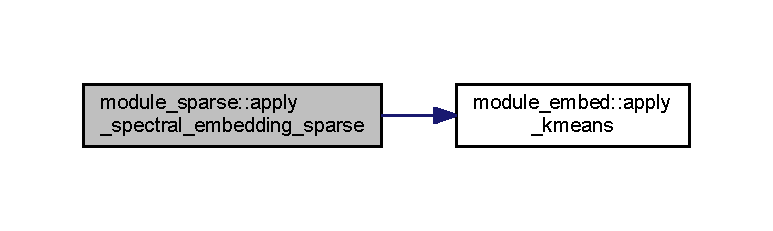
\includegraphics[width=350pt]{namespacemodule__sparse_a6fc2f45f94f4ea124ea27f88b8823274_cgraph}
\end{center}
\end{figure}




Here is the caller graph for this function\+:\nopagebreak
\begin{figure}[H]
\begin{center}
\leavevmode
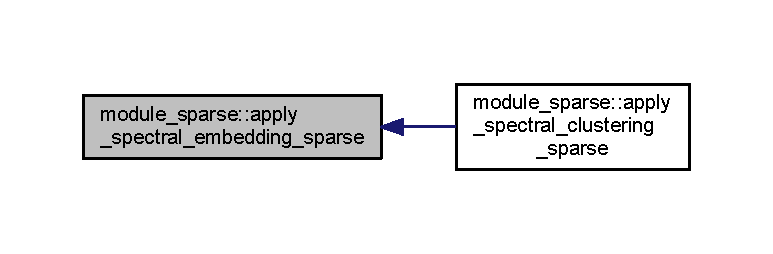
\includegraphics[width=350pt]{namespacemodule__sparse_a6fc2f45f94f4ea124ea27f88b8823274_icgraph}
\end{center}
\end{figure}


\hypertarget{namespacemodule__sparse_a172821d54ec6f3bec6f07ca4f9d96d37}{}\index{module\+\_\+sparse@{module\+\_\+sparse}!compute\+\_\+matvec\+\_\+prod@{compute\+\_\+matvec\+\_\+prod}}
\index{compute\+\_\+matvec\+\_\+prod@{compute\+\_\+matvec\+\_\+prod}!module\+\_\+sparse@{module\+\_\+sparse}}
\subsubsection[{compute\+\_\+matvec\+\_\+prod}]{\setlength{\rightskip}{0pt plus 5cm}subroutine module\+\_\+sparse\+::compute\+\_\+matvec\+\_\+prod (
\begin{DoxyParamCaption}
\item[{double precision, dimension(nnz), intent(in)}]{A, }
\item[{integer, dimension(nnz), intent(in)}]{I\+A, }
\item[{integer, dimension(nnz), intent(in)}]{J\+A, }
\item[{double precision, dimension(n), intent(in)}]{X, }
\item[{double precision, dimension(n), intent(out)}]{Y, }
\item[{integer, intent(in)}]{n, }
\item[{integer, intent(in)}]{nnz}
\end{DoxyParamCaption}
)}\label{namespacemodule__sparse_a172821d54ec6f3bec6f07ca4f9d96d37}


Computes the matrix vector product using sparsity. 


\begin{DoxyParams}[1]{Parameters}
\mbox{\tt in}  & {\em A} & the sparse matrix \\
\hline
\mbox{\tt in}  & {\em X} & the input vector \\
\hline
\mbox{\tt in}  & {\em n} & \\
\hline
\mbox{\tt in}  & {\em nnz} & the number of non-\/zero coefficients \\
\hline
\mbox{\tt in}  & {\em I\+A} & the row indices of the matrix coefficients \\
\hline
\mbox{\tt in}  & {\em J\+A} & the column indices of the matrix coefficients \\
\hline
\mbox{\tt out}  & {\em Y} & the resulting vector \\
\hline
\end{DoxyParams}


Here is the caller graph for this function\+:\nopagebreak
\begin{figure}[H]
\begin{center}
\leavevmode
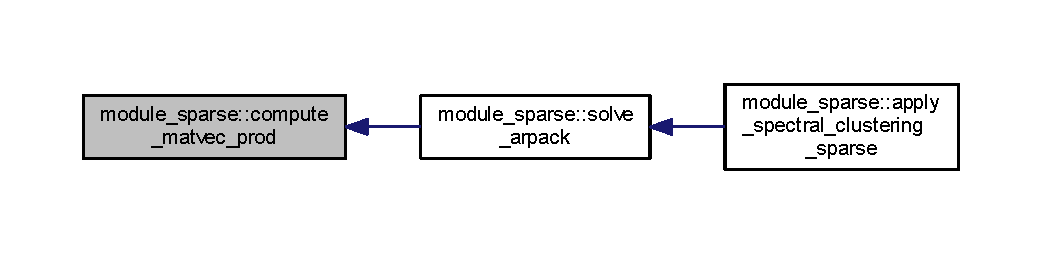
\includegraphics[width=350pt]{namespacemodule__sparse_a172821d54ec6f3bec6f07ca4f9d96d37_icgraph}
\end{center}
\end{figure}


\hypertarget{namespacemodule__sparse_a1945ecdb844a637fd6372b3686b4df40}{}\index{module\+\_\+sparse@{module\+\_\+sparse}!solve\+\_\+arpack@{solve\+\_\+arpack}}
\index{solve\+\_\+arpack@{solve\+\_\+arpack}!module\+\_\+sparse@{module\+\_\+sparse}}
\subsubsection[{solve\+\_\+arpack}]{\setlength{\rightskip}{0pt plus 5cm}subroutine module\+\_\+sparse\+::solve\+\_\+arpack (
\begin{DoxyParamCaption}
\item[{double precision, dimension(\+:), intent(in)}]{A, }
\item[{integer, dimension(\+:), intent(in)}]{I\+A, }
\item[{integer, dimension(\+:), intent(in)}]{J\+A, }
\item[{integer, intent(in)}]{dim, }
\item[{integer, intent(in)}]{nnz, }
\item[{integer, intent(in)}]{nb\+\_\+clusters\+\_\+max, }
\item[{double precision, dimension(\+:), intent(out), pointer}]{W, }
\item[{double precision, dimension(\+:,\+:), intent(out), pointer}]{Z}
\end{DoxyParamCaption}
)}\label{namespacemodule__sparse_a1945ecdb844a637fd6372b3686b4df40}

\begin{DoxyParams}[1]{Parameters}
\mbox{\tt in}  & {\em A} & the affinity sparse matrix \\
\hline
\mbox{\tt in}  & {\em dim} & the number of spatial dimensions \\
\hline
\mbox{\tt in}  & {\em dim} & the number of spatial dimensions \\
\hline
\mbox{\tt in}  & {\em dim} & \\
\hline
\mbox{\tt in}  & {\em nb\+\_\+clusters\+\_\+max} & the maximum number of clusters \\
\hline
\mbox{\tt in}  & {\em nnz} & the number of non-\/zero coefficients \\
\hline
\mbox{\tt in}  & {\em I\+A} & the row indices of the affinity matrix coefficients \\
\hline
\mbox{\tt in}  & {\em J\+A} & the column indices of the affinity matrix coefficients \\
\hline
\mbox{\tt out}  & {\em Z} & the matrix of eigen vectors \\
\hline
\mbox{\tt out}  & {\em W} & \\
\hline
\end{DoxyParams}


Here is the call graph for this function\+:\nopagebreak
\begin{figure}[H]
\begin{center}
\leavevmode
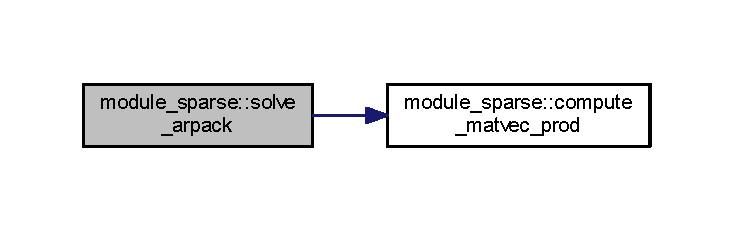
\includegraphics[width=350pt]{namespacemodule__sparse_a1945ecdb844a637fd6372b3686b4df40_cgraph}
\end{center}
\end{figure}




Here is the caller graph for this function\+:\nopagebreak
\begin{figure}[H]
\begin{center}
\leavevmode
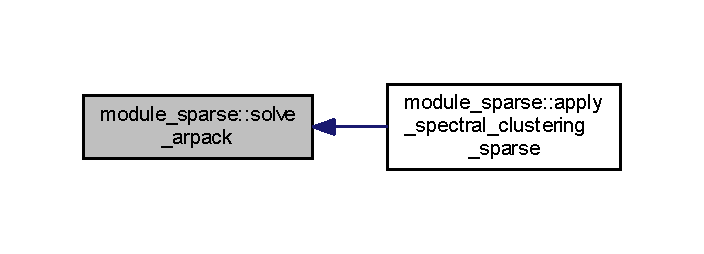
\includegraphics[width=338pt]{namespacemodule__sparse_a1945ecdb844a637fd6372b3686b4df40_icgraph}
\end{center}
\end{figure}



\hypertarget{namespacemodule__structure}{}\section{module\+\_\+structure Module Reference}
\label{namespacemodule__structure}\index{module\+\_\+structure@{module\+\_\+structure}}


Contains structure types required by the different modules.  


\subsection*{Data Types}
\begin{DoxyCompactItemize}
\item 
type \hyperlink{structmodule__structure_1_1type__clustering__param}{type\+\_\+clustering\+\_\+param}
\item 
type \hyperlink{structmodule__structure_1_1type__clusters}{type\+\_\+clusters}
\item 
type \hyperlink{structmodule__structure_1_1type__data}{type\+\_\+data}
\item 
type \hyperlink{structmodule__structure_1_1type__points}{type\+\_\+points}
\end{DoxyCompactItemize}


\subsection{Detailed Description}
Contains structure types required by the different modules. 
\hypertarget{namespacemodule__teste__clusters}{}\section{module\+\_\+teste\+\_\+clusters Module Reference}
\label{namespacemodule__teste__clusters}\index{module\+\_\+teste\+\_\+clusters@{module\+\_\+teste\+\_\+clusters}}
\subsection*{Data Types}
\begin{DoxyCompactItemize}
\item 
type \hyperlink{structmodule__teste__clusters_1_1type__test}{type\+\_\+test}
\end{DoxyCompactItemize}
\subsection*{Functions/\+Subroutines}
\begin{DoxyCompactItemize}
\item 
subroutine \hyperlink{namespacemodule__teste__clusters_aea89e91184c2a89eec2fd785671663f9}{create\+\_\+executable} (test)
\begin{DoxyCompactList}\small\item\em Creates an executable called {\itshape go} for runcluster. \end{DoxyCompactList}\item 
subroutine \hyperlink{namespacemodule__teste__clusters_aaf3c23842ff04fc92eebd8688fe74d70}{create\+\_\+test} (test)
\begin{DoxyCompactList}\small\item\em Creates a test file. \end{DoxyCompactList}\item 
subroutine \hyperlink{namespacemodule__teste__clusters_a9ab3f7278117b04c1ba94ff7cd96e3d2}{execute\+\_\+test} (test)
\begin{DoxyCompactList}\small\item\em Executes the script {\itshape go} and displays information on the console screen. \end{DoxyCompactList}\item 
subroutine \hyperlink{namespacemodule__teste__clusters_aa745f9e68594bf01494b5de549240cf8}{create\+\_\+data}
\begin{DoxyCompactList}\small\item\em Generates an example of a raw geometric data file for testing purpose. \end{DoxyCompactList}\end{DoxyCompactItemize}


\subsection{Function/\+Subroutine Documentation}
\hypertarget{namespacemodule__teste__clusters_aa745f9e68594bf01494b5de549240cf8}{}\index{module\+\_\+teste\+\_\+clusters@{module\+\_\+teste\+\_\+clusters}!create\+\_\+data@{create\+\_\+data}}
\index{create\+\_\+data@{create\+\_\+data}!module\+\_\+teste\+\_\+clusters@{module\+\_\+teste\+\_\+clusters}}
\subsubsection[{create\+\_\+data}]{\setlength{\rightskip}{0pt plus 5cm}subroutine module\+\_\+teste\+\_\+clusters\+::create\+\_\+data (
\begin{DoxyParamCaption}
{}
\end{DoxyParamCaption}
)}\label{namespacemodule__teste__clusters_aa745f9e68594bf01494b5de549240cf8}


Generates an example of a raw geometric data file for testing purpose. 

\hypertarget{namespacemodule__teste__clusters_aea89e91184c2a89eec2fd785671663f9}{}\index{module\+\_\+teste\+\_\+clusters@{module\+\_\+teste\+\_\+clusters}!create\+\_\+executable@{create\+\_\+executable}}
\index{create\+\_\+executable@{create\+\_\+executable}!module\+\_\+teste\+\_\+clusters@{module\+\_\+teste\+\_\+clusters}}
\subsubsection[{create\+\_\+executable}]{\setlength{\rightskip}{0pt plus 5cm}subroutine module\+\_\+teste\+\_\+clusters\+::create\+\_\+executable (
\begin{DoxyParamCaption}
\item[{type({\bf type\+\_\+test})}]{test}
\end{DoxyParamCaption}
)}\label{namespacemodule__teste__clusters_aea89e91184c2a89eec2fd785671663f9}


Creates an executable called {\itshape go} for runcluster. 


\begin{DoxyParams}[1]{Parameters}
\mbox{\tt in}  & {\em test} & \\
\hline
\end{DoxyParams}
\hypertarget{namespacemodule__teste__clusters_aaf3c23842ff04fc92eebd8688fe74d70}{}\index{module\+\_\+teste\+\_\+clusters@{module\+\_\+teste\+\_\+clusters}!create\+\_\+test@{create\+\_\+test}}
\index{create\+\_\+test@{create\+\_\+test}!module\+\_\+teste\+\_\+clusters@{module\+\_\+teste\+\_\+clusters}}
\subsubsection[{create\+\_\+test}]{\setlength{\rightskip}{0pt plus 5cm}subroutine module\+\_\+teste\+\_\+clusters\+::create\+\_\+test (
\begin{DoxyParamCaption}
\item[{type({\bf type\+\_\+test})}]{test}
\end{DoxyParamCaption}
)}\label{namespacemodule__teste__clusters_aaf3c23842ff04fc92eebd8688fe74d70}


Creates a test file. 


\begin{DoxyParams}[1]{Parameters}
\mbox{\tt in}  & {\em test} & \\
\hline
\end{DoxyParams}
\hypertarget{namespacemodule__teste__clusters_a9ab3f7278117b04c1ba94ff7cd96e3d2}{}\index{module\+\_\+teste\+\_\+clusters@{module\+\_\+teste\+\_\+clusters}!execute\+\_\+test@{execute\+\_\+test}}
\index{execute\+\_\+test@{execute\+\_\+test}!module\+\_\+teste\+\_\+clusters@{module\+\_\+teste\+\_\+clusters}}
\subsubsection[{execute\+\_\+test}]{\setlength{\rightskip}{0pt plus 5cm}subroutine module\+\_\+teste\+\_\+clusters\+::execute\+\_\+test (
\begin{DoxyParamCaption}
\item[{type({\bf type\+\_\+test})}]{test}
\end{DoxyParamCaption}
)}\label{namespacemodule__teste__clusters_a9ab3f7278117b04c1ba94ff7cd96e3d2}


Executes the script {\itshape go} and displays information on the console screen. 


\begin{DoxyParams}[1]{Parameters}
\mbox{\tt in}  & {\em test} & \\
\hline
\end{DoxyParams}

\hypertarget{namespacemodule__visuclusters}{}\section{module\+\_\+visuclusters Module Reference}
\label{namespacemodule__visuclusters}\index{module\+\_\+visuclusters@{module\+\_\+visuclusters}}


Contains methods enabling writing results in a selected data file format (for now \+: Paraview or G\+M\+S\+H)  


\subsection*{Functions/\+Subroutines}
\begin{DoxyCompactItemize}
\item 
subroutine \hyperlink{namespacemodule__visuclusters_ab68939a34024c66e1e7cc64a0dcf8736}{read\+\_\+metadata} (params)
\begin{DoxyCompactList}\small\item\em Reads a file containing metadata on the data and the computed clusters. \end{DoxyCompactList}\item 
subroutine \hyperlink{namespacemodule__visuclusters_adae3f4360febb54cb901ce9f591d8656}{write\+\_\+partitioning} (format\+\_\+output, params)
\begin{DoxyCompactList}\small\item\em Writes the geometry of the partitioning (Gmsh or Paraview) and calls the eponym function. \end{DoxyCompactList}\item 
subroutine \hyperlink{namespacemodule__visuclusters_a11320cacc6eae8f372b75e9ec61b38b6}{write\+\_\+assignment} (format\+\_\+output, params)
\begin{DoxyCompactList}\small\item\em Initializes the file of the partitionning. \end{DoxyCompactList}\item 
subroutine \hyperlink{namespacemodule__visuclusters_a426807700ec2991178bd989694a2ff17}{write\+\_\+partial\+\_\+clusters} (format\+\_\+output, params)
\begin{DoxyCompactList}\small\item\em Writes the clusters before grouping by calling the corresponding method (Gmsh or Paraview) \end{DoxyCompactList}\item 
subroutine \hyperlink{namespacemodule__visuclusters_adf901cfd1bc769cadd3558369594b074}{write\+\_\+final\+\_\+clusters} (format\+\_\+output, params)
\begin{DoxyCompactList}\small\item\em Writes the clusters after grouping by calling the corresponding method (Gmsh or Paraview) \end{DoxyCompactList}\item 
subroutine \hyperlink{namespacemodule__visuclusters_aeed2c5753cf8c47dadf20e55474c830b}{list\+\_\+commands} (format\+\_\+output)
\begin{DoxyCompactList}\small\item\em Lists the commands related to Gmsh or Paraview depending on the input parameter. \end{DoxyCompactList}\end{DoxyCompactItemize}


\subsection{Detailed Description}
Contains methods enabling writing results in a selected data file format (for now \+: Paraview or G\+M\+S\+H) 

\subsection{Function/\+Subroutine Documentation}
\hypertarget{namespacemodule__visuclusters_aeed2c5753cf8c47dadf20e55474c830b}{}\index{module\+\_\+visuclusters@{module\+\_\+visuclusters}!list\+\_\+commands@{list\+\_\+commands}}
\index{list\+\_\+commands@{list\+\_\+commands}!module\+\_\+visuclusters@{module\+\_\+visuclusters}}
\subsubsection[{list\+\_\+commands}]{\setlength{\rightskip}{0pt plus 5cm}subroutine module\+\_\+visuclusters\+::list\+\_\+commands (
\begin{DoxyParamCaption}
\item[{character (len=30)}]{format\+\_\+output}
\end{DoxyParamCaption}
)}\label{namespacemodule__visuclusters_aeed2c5753cf8c47dadf20e55474c830b}


Lists the commands related to Gmsh or Paraview depending on the input parameter. 


\begin{DoxyParams}[1]{Parameters}
\mbox{\tt in}  & {\em format\+\_\+output} & the file format for visualization \\
\hline
\end{DoxyParams}


Here is the call graph for this function\+:\nopagebreak
\begin{figure}[H]
\begin{center}
\leavevmode
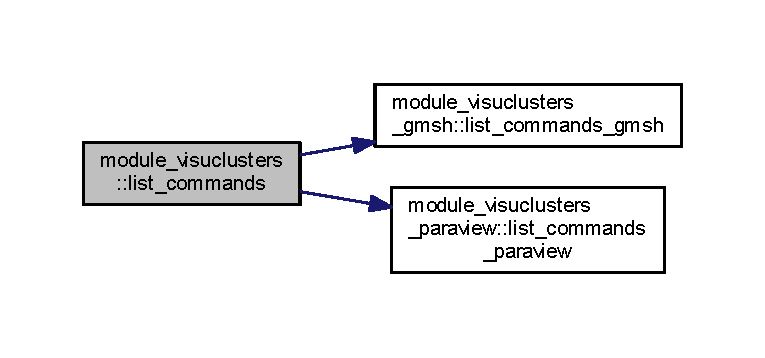
\includegraphics[width=350pt]{namespacemodule__visuclusters_aeed2c5753cf8c47dadf20e55474c830b_cgraph}
\end{center}
\end{figure}


\hypertarget{namespacemodule__visuclusters_ab68939a34024c66e1e7cc64a0dcf8736}{}\index{module\+\_\+visuclusters@{module\+\_\+visuclusters}!read\+\_\+metadata@{read\+\_\+metadata}}
\index{read\+\_\+metadata@{read\+\_\+metadata}!module\+\_\+visuclusters@{module\+\_\+visuclusters}}
\subsubsection[{read\+\_\+metadata}]{\setlength{\rightskip}{0pt plus 5cm}subroutine module\+\_\+visuclusters\+::read\+\_\+metadata (
\begin{DoxyParamCaption}
\item[{type({\bf type\+\_\+params})}]{params}
\end{DoxyParamCaption}
)}\label{namespacemodule__visuclusters_ab68939a34024c66e1e7cc64a0dcf8736}


Reads a file containing metadata on the data and the computed clusters. 

This function extracts the following information from the input {\itshape fort.\+3} file \+: 
\begin{DoxyEnumerate}
\item The data file name  
\item The number of the points in the entire data set  
\item The number of processes used  
\item The partitioning mode (by interface or overlapping)  
\item The number of clusters found  
\item The data file format  
\end{DoxyEnumerate}In the case of a picture format\+: this extra information is written \+: 
\begin{DoxyEnumerate}
\item The image dimension  
\item The image partitioning  
\item The number of attributes  
\item The number of steps (only in geometric format)  
\end{DoxyEnumerate}\begin{DoxySeeAlso}{See also}
\hyperlink{namespacemodule__sortie_a3093c50035046621188d9a0da3b8a587}{write\+\_\+metadata()} 
\end{DoxySeeAlso}

\begin{DoxyParams}[1]{Parameters}
\mbox{\tt in,out}  & {\em params} & the parameters defined in the \textit{param.in} file \\
\hline
\end{DoxyParams}
\hypertarget{namespacemodule__visuclusters_a11320cacc6eae8f372b75e9ec61b38b6}{}\index{module\+\_\+visuclusters@{module\+\_\+visuclusters}!write\+\_\+assignment@{write\+\_\+assignment}}
\index{write\+\_\+assignment@{write\+\_\+assignment}!module\+\_\+visuclusters@{module\+\_\+visuclusters}}
\subsubsection[{write\+\_\+assignment}]{\setlength{\rightskip}{0pt plus 5cm}subroutine module\+\_\+visuclusters\+::write\+\_\+assignment (
\begin{DoxyParamCaption}
\item[{character (len=30)}]{format\+\_\+output, }
\item[{type({\bf type\+\_\+params})}]{params}
\end{DoxyParamCaption}
)}\label{namespacemodule__visuclusters_a11320cacc6eae8f372b75e9ec61b38b6}


Initializes the file of the partitionning. 

This method extracts details on partitioning from the {\itshape decoupe.\+x} files. \begin{DoxySeeAlso}{See also}
\hyperlink{namespacemodule__visuclusters_a426807700ec2991178bd989694a2ff17}{module\+\_\+calcul\+::write\+\_\+partial\+\_\+clusters()} 
\end{DoxySeeAlso}

\begin{DoxyParams}[1]{Parameters}
\mbox{\tt in}  & {\em params} & the parameters defined in the \textit{param.in} file \\
\hline
\mbox{\tt in}  & {\em format\+\_\+output} & the file format for visualization \\
\hline
\end{DoxyParams}


Here is the call graph for this function\+:\nopagebreak
\begin{figure}[H]
\begin{center}
\leavevmode
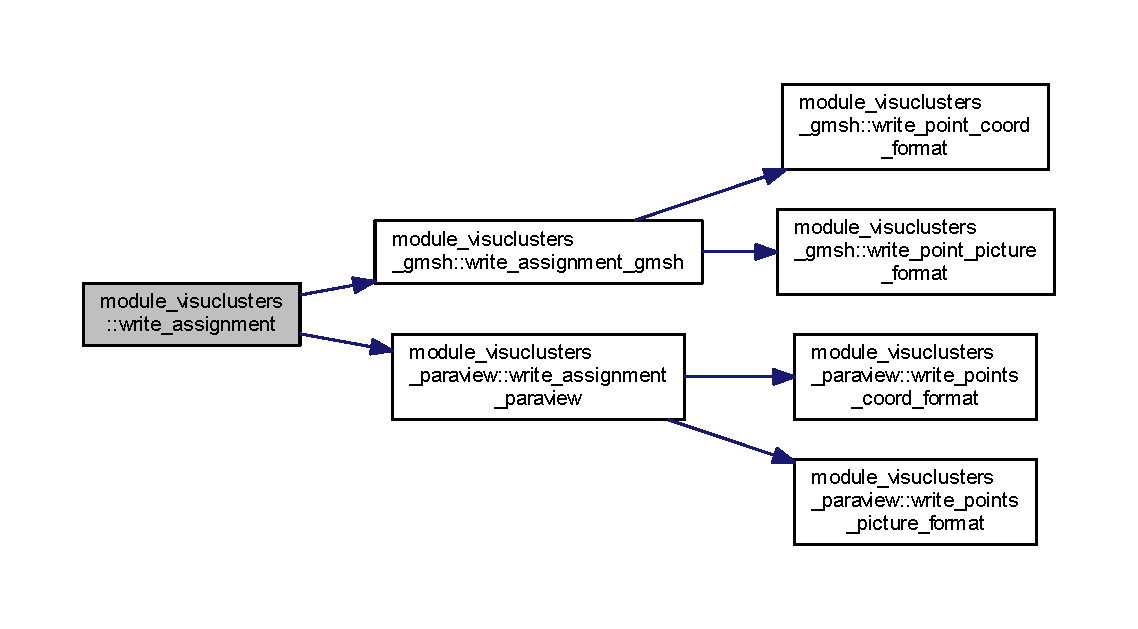
\includegraphics[width=350pt]{namespacemodule__visuclusters_a11320cacc6eae8f372b75e9ec61b38b6_cgraph}
\end{center}
\end{figure}


\hypertarget{namespacemodule__visuclusters_adf901cfd1bc769cadd3558369594b074}{}\index{module\+\_\+visuclusters@{module\+\_\+visuclusters}!write\+\_\+final\+\_\+clusters@{write\+\_\+final\+\_\+clusters}}
\index{write\+\_\+final\+\_\+clusters@{write\+\_\+final\+\_\+clusters}!module\+\_\+visuclusters@{module\+\_\+visuclusters}}
\subsubsection[{write\+\_\+final\+\_\+clusters}]{\setlength{\rightskip}{0pt plus 5cm}subroutine module\+\_\+visuclusters\+::write\+\_\+final\+\_\+clusters (
\begin{DoxyParamCaption}
\item[{character (len=30)}]{format\+\_\+output, }
\item[{type({\bf type\+\_\+params})}]{params}
\end{DoxyParamCaption}
)}\label{namespacemodule__visuclusters_adf901cfd1bc769cadd3558369594b074}


Writes the clusters after grouping by calling the corresponding method (Gmsh or Paraview) 

This methods extracts details on computed clusters from {\itshape cluster.\+final.\+x} files. \begin{DoxySeeAlso}{See also}
\hyperlink{namespacemodule__visuclusters_adf901cfd1bc769cadd3558369594b074}{module\+\_\+calcul\+::write\+\_\+final\+\_\+clusters()} 
\end{DoxySeeAlso}

\begin{DoxyParams}[1]{Parameters}
\mbox{\tt in}  & {\em params} & the parameters defined in the \textit{param.in} file \\
\hline
\mbox{\tt in}  & {\em format\+\_\+output} & the file format for visualization \\
\hline
\end{DoxyParams}


Here is the call graph for this function\+:\nopagebreak
\begin{figure}[H]
\begin{center}
\leavevmode
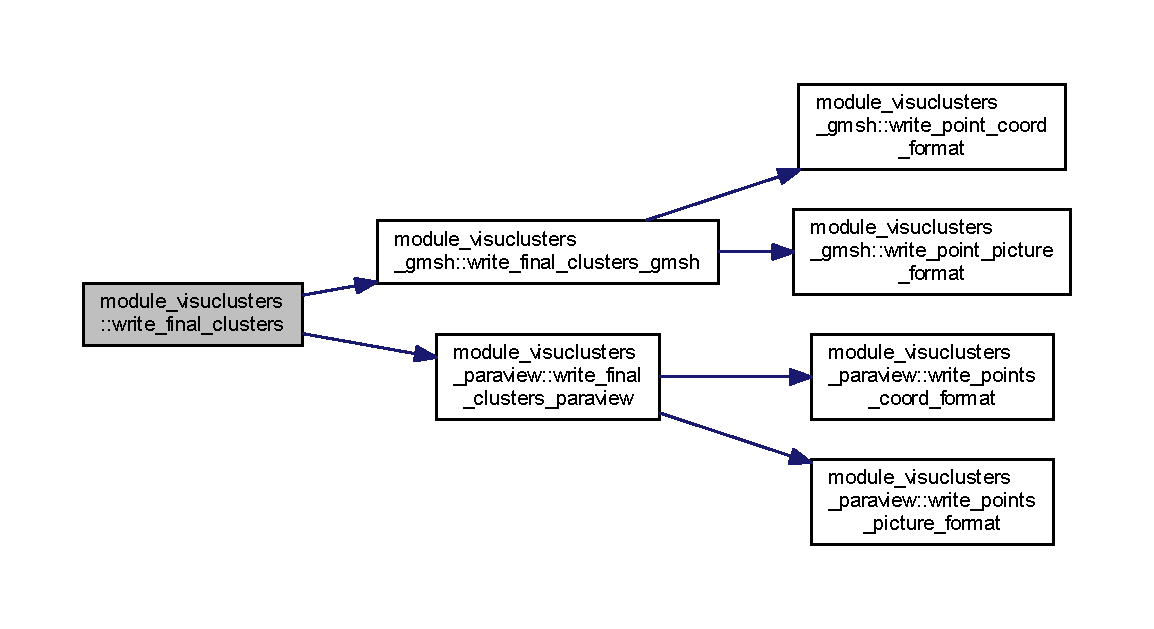
\includegraphics[width=350pt]{namespacemodule__visuclusters_adf901cfd1bc769cadd3558369594b074_cgraph}
\end{center}
\end{figure}


\hypertarget{namespacemodule__visuclusters_a426807700ec2991178bd989694a2ff17}{}\index{module\+\_\+visuclusters@{module\+\_\+visuclusters}!write\+\_\+partial\+\_\+clusters@{write\+\_\+partial\+\_\+clusters}}
\index{write\+\_\+partial\+\_\+clusters@{write\+\_\+partial\+\_\+clusters}!module\+\_\+visuclusters@{module\+\_\+visuclusters}}
\subsubsection[{write\+\_\+partial\+\_\+clusters}]{\setlength{\rightskip}{0pt plus 5cm}subroutine module\+\_\+visuclusters\+::write\+\_\+partial\+\_\+clusters (
\begin{DoxyParamCaption}
\item[{character (len=30)}]{format\+\_\+output, }
\item[{type({\bf type\+\_\+params})}]{params}
\end{DoxyParamCaption}
)}\label{namespacemodule__visuclusters_a426807700ec2991178bd989694a2ff17}


Writes the clusters before grouping by calling the corresponding method (Gmsh or Paraview) 

This methods extracts details on computed clusters on each domain from {\itshape cluster.\+partiel.\+x} files. \begin{DoxySeeAlso}{See also}
\hyperlink{namespacemodule__visuclusters_a426807700ec2991178bd989694a2ff17}{module\+\_\+calcul\+::write\+\_\+partial\+\_\+clusters()} 
\end{DoxySeeAlso}

\begin{DoxyParams}[1]{Parameters}
\mbox{\tt in}  & {\em params} & the parameters defined in the \textit{param.in} file \\
\hline
\mbox{\tt in}  & {\em format\+\_\+output} & the file format for visualization \\
\hline
\end{DoxyParams}


Here is the call graph for this function\+:\nopagebreak
\begin{figure}[H]
\begin{center}
\leavevmode
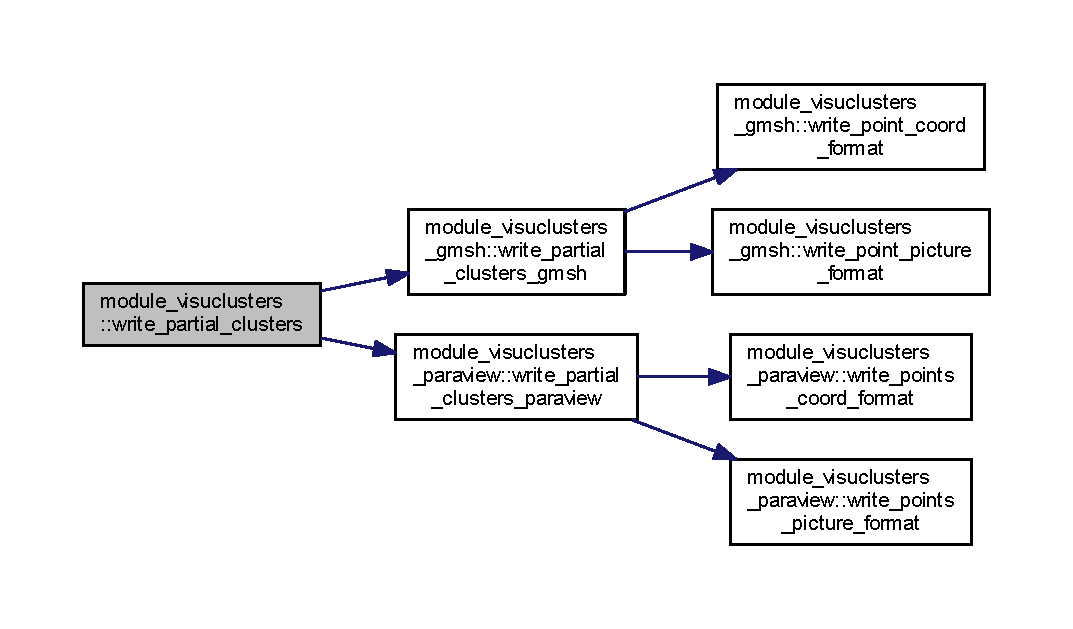
\includegraphics[width=350pt]{namespacemodule__visuclusters_a426807700ec2991178bd989694a2ff17_cgraph}
\end{center}
\end{figure}


\hypertarget{namespacemodule__visuclusters_adae3f4360febb54cb901ce9f591d8656}{}\index{module\+\_\+visuclusters@{module\+\_\+visuclusters}!write\+\_\+partitioning@{write\+\_\+partitioning}}
\index{write\+\_\+partitioning@{write\+\_\+partitioning}!module\+\_\+visuclusters@{module\+\_\+visuclusters}}
\subsubsection[{write\+\_\+partitioning}]{\setlength{\rightskip}{0pt plus 5cm}subroutine module\+\_\+visuclusters\+::write\+\_\+partitioning (
\begin{DoxyParamCaption}
\item[{character (len=30)}]{format\+\_\+output, }
\item[{type({\bf type\+\_\+params})}]{params}
\end{DoxyParamCaption}
)}\label{namespacemodule__visuclusters_adae3f4360febb54cb901ce9f591d8656}


Writes the geometry of the partitioning (Gmsh or Paraview) and calls the eponym function. 

This methods extracts the domain definitions from the {\itshape fort.\+2} file. \begin{DoxySeeAlso}{See also}
\hyperlink{namespacemodule__visuclusters_adae3f4360febb54cb901ce9f591d8656}{module\+\_\+calcul\+::write\+\_\+partitioning()} 
\end{DoxySeeAlso}

\begin{DoxyParams}[1]{Parameters}
\mbox{\tt in}  & {\em params} & the parameters defined in the \textit{param.in} file \\
\hline
\mbox{\tt in}  & {\em format\+\_\+output} & the file format for visualization \\
\hline
\end{DoxyParams}


Here is the call graph for this function\+:\nopagebreak
\begin{figure}[H]
\begin{center}
\leavevmode
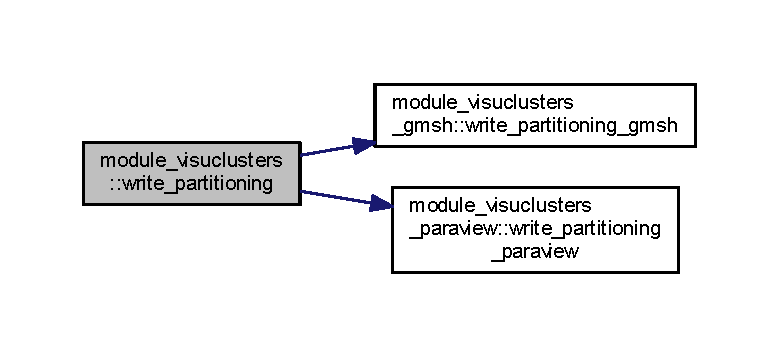
\includegraphics[width=350pt]{namespacemodule__visuclusters_adae3f4360febb54cb901ce9f591d8656_cgraph}
\end{center}
\end{figure}



\hypertarget{namespacemodule__visuclusters__gmsh}{}\section{module\+\_\+visuclusters\+\_\+gmsh Module Reference}
\label{namespacemodule__visuclusters__gmsh}\index{module\+\_\+visuclusters\+\_\+gmsh@{module\+\_\+visuclusters\+\_\+gmsh}}


Contains methods enabling writing results in file specifically formatted for G\+M\+S\+H.  


\subsection*{Functions/\+Subroutines}
\begin{DoxyCompactItemize}
\item 
subroutine \hyperlink{namespacemodule__visuclusters__gmsh_a2ffd04d2e2dcdda290446affaf3a76dc}{write\+\_\+partitioning\+\_\+gmsh} (params)
\begin{DoxyCompactList}\small\item\em Writes the geometry partitioning for Gmsh visualization. \end{DoxyCompactList}\item 
subroutine \hyperlink{namespacemodule__visuclusters__gmsh_a3771400a4e195904654e041eef83247f}{write\+\_\+assignment\+\_\+gmsh} (params)
\begin{DoxyCompactList}\small\item\em Initializes the file of the partitioning for Gmsh visualization. \end{DoxyCompactList}\item 
subroutine \hyperlink{namespacemodule__visuclusters__gmsh_af04ca060cedb92fb755fd6cbb1330011}{write\+\_\+partial\+\_\+clusters\+\_\+gmsh} (params)
\begin{DoxyCompactList}\small\item\em Writes the clusters before grouping for Gmsh visualization. \end{DoxyCompactList}\item 
subroutine \hyperlink{namespacemodule__visuclusters__gmsh_a3fe1790e0267b255e689ead80e6c8ca8}{write\+\_\+final\+\_\+clusters\+\_\+gmsh} (params)
\begin{DoxyCompactList}\small\item\em Writes the clusters after grouping for Gmsh visualization. \end{DoxyCompactList}\item 
subroutine \hyperlink{namespacemodule__visuclusters__gmsh_ab3a87863baf4bd33953b9aa7950d5d26}{write\+\_\+point\+\_\+coord\+\_\+format} (unit, dim, coords, id, k)
\begin{DoxyCompactList}\small\item\em Writes point coordinates from coordinates format for Gmsh visualization. \end{DoxyCompactList}\item 
subroutine \hyperlink{namespacemodule__visuclusters__gmsh_aa00f636e7ea0ae13557bdf9fa21b285f}{write\+\_\+point\+\_\+picture\+\_\+format} (unit, params, id, k)
\begin{DoxyCompactList}\small\item\em Writes point coordinates from picture format for Gmsh visualization. \end{DoxyCompactList}\item 
subroutine \hyperlink{namespacemodule__visuclusters__gmsh_af4df8b9f65af2acfbc5489b6e299cfde}{list\+\_\+commands\+\_\+gmsh}
\begin{DoxyCompactList}\small\item\em Lists the commands related to Gmsh visualization. \end{DoxyCompactList}\end{DoxyCompactItemize}


\subsection{Detailed Description}
Contains methods enabling writing results in file specifically formatted for G\+M\+S\+H. 

\subsection{Function/\+Subroutine Documentation}
\hypertarget{namespacemodule__visuclusters__gmsh_af4df8b9f65af2acfbc5489b6e299cfde}{}\index{module\+\_\+visuclusters\+\_\+gmsh@{module\+\_\+visuclusters\+\_\+gmsh}!list\+\_\+commands\+\_\+gmsh@{list\+\_\+commands\+\_\+gmsh}}
\index{list\+\_\+commands\+\_\+gmsh@{list\+\_\+commands\+\_\+gmsh}!module\+\_\+visuclusters\+\_\+gmsh@{module\+\_\+visuclusters\+\_\+gmsh}}
\subsubsection[{list\+\_\+commands\+\_\+gmsh}]{\setlength{\rightskip}{0pt plus 5cm}subroutine module\+\_\+visuclusters\+\_\+gmsh\+::list\+\_\+commands\+\_\+gmsh (
\begin{DoxyParamCaption}
{}
\end{DoxyParamCaption}
)}\label{namespacemodule__visuclusters__gmsh_af4df8b9f65af2acfbc5489b6e299cfde}


Lists the commands related to Gmsh visualization. 



Here is the caller graph for this function\+:\nopagebreak
\begin{figure}[H]
\begin{center}
\leavevmode
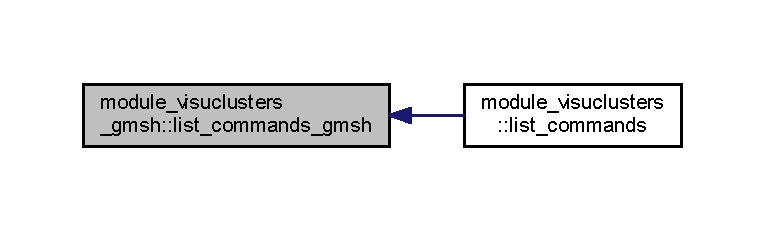
\includegraphics[width=350pt]{namespacemodule__visuclusters__gmsh_af4df8b9f65af2acfbc5489b6e299cfde_icgraph}
\end{center}
\end{figure}


\hypertarget{namespacemodule__visuclusters__gmsh_a3771400a4e195904654e041eef83247f}{}\index{module\+\_\+visuclusters\+\_\+gmsh@{module\+\_\+visuclusters\+\_\+gmsh}!write\+\_\+assignment\+\_\+gmsh@{write\+\_\+assignment\+\_\+gmsh}}
\index{write\+\_\+assignment\+\_\+gmsh@{write\+\_\+assignment\+\_\+gmsh}!module\+\_\+visuclusters\+\_\+gmsh@{module\+\_\+visuclusters\+\_\+gmsh}}
\subsubsection[{write\+\_\+assignment\+\_\+gmsh}]{\setlength{\rightskip}{0pt plus 5cm}subroutine module\+\_\+visuclusters\+\_\+gmsh\+::write\+\_\+assignment\+\_\+gmsh (
\begin{DoxyParamCaption}
\item[{type({\bf type\+\_\+params})}]{params}
\end{DoxyParamCaption}
)}\label{namespacemodule__visuclusters__gmsh_a3771400a4e195904654e041eef83247f}


Initializes the file of the partitioning for Gmsh visualization. 

This method extracts details on partitioning from the {\itshape decoupe.\+x} files and writes them in {\itshape decoupe.\+visu} file. \begin{DoxyNote}{Note}
{\itshape x} is the identifier (number) of a process. 
\end{DoxyNote}
\begin{DoxySeeAlso}{See also}
\hyperlink{namespacemodule__sortie_abd1cdf529e5c71b3186c8d980e3d5117}{write\+\_\+partitioning()} 
\end{DoxySeeAlso}

\begin{DoxyParams}[1]{Parameters}
\mbox{\tt in}  & {\em params} & the parameters defined in the \textit{param.in} file \\
\hline
\end{DoxyParams}


Here is the call graph for this function\+:\nopagebreak
\begin{figure}[H]
\begin{center}
\leavevmode
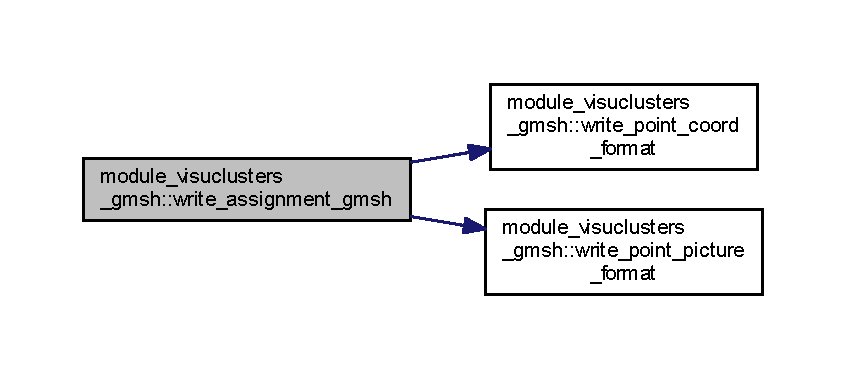
\includegraphics[width=350pt]{namespacemodule__visuclusters__gmsh_a3771400a4e195904654e041eef83247f_cgraph}
\end{center}
\end{figure}




Here is the caller graph for this function\+:\nopagebreak
\begin{figure}[H]
\begin{center}
\leavevmode
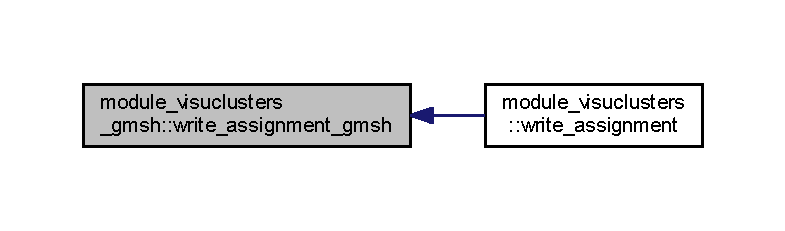
\includegraphics[width=350pt]{namespacemodule__visuclusters__gmsh_a3771400a4e195904654e041eef83247f_icgraph}
\end{center}
\end{figure}


\hypertarget{namespacemodule__visuclusters__gmsh_a3fe1790e0267b255e689ead80e6c8ca8}{}\index{module\+\_\+visuclusters\+\_\+gmsh@{module\+\_\+visuclusters\+\_\+gmsh}!write\+\_\+final\+\_\+clusters\+\_\+gmsh@{write\+\_\+final\+\_\+clusters\+\_\+gmsh}}
\index{write\+\_\+final\+\_\+clusters\+\_\+gmsh@{write\+\_\+final\+\_\+clusters\+\_\+gmsh}!module\+\_\+visuclusters\+\_\+gmsh@{module\+\_\+visuclusters\+\_\+gmsh}}
\subsubsection[{write\+\_\+final\+\_\+clusters\+\_\+gmsh}]{\setlength{\rightskip}{0pt plus 5cm}subroutine module\+\_\+visuclusters\+\_\+gmsh\+::write\+\_\+final\+\_\+clusters\+\_\+gmsh (
\begin{DoxyParamCaption}
\item[{type({\bf type\+\_\+params})}]{params}
\end{DoxyParamCaption}
)}\label{namespacemodule__visuclusters__gmsh_a3fe1790e0267b255e689ead80e6c8ca8}


Writes the clusters after grouping for Gmsh visualization. 

This methods extracts details on computed clusters from {\itshape cluster.\+final.\+x} files and writes them in {\itshape cluster.\+final.\+visu} file. \begin{DoxyNote}{Note}
{\itshape x} is the identifier (number) of a cluster. 
\end{DoxyNote}
\begin{DoxySeeAlso}{See also}
\hyperlink{namespacemodule__sortie_a819ceed76e9600e8eec63a7b730d1d92}{module\+\_\+calcul\+::write\+\_\+final\+\_\+clusters()} 
\end{DoxySeeAlso}

\begin{DoxyParams}[1]{Parameters}
\mbox{\tt in}  & {\em params} & the parameters defined in the \textit{param.in} file \\
\hline
\end{DoxyParams}


Here is the call graph for this function\+:\nopagebreak
\begin{figure}[H]
\begin{center}
\leavevmode
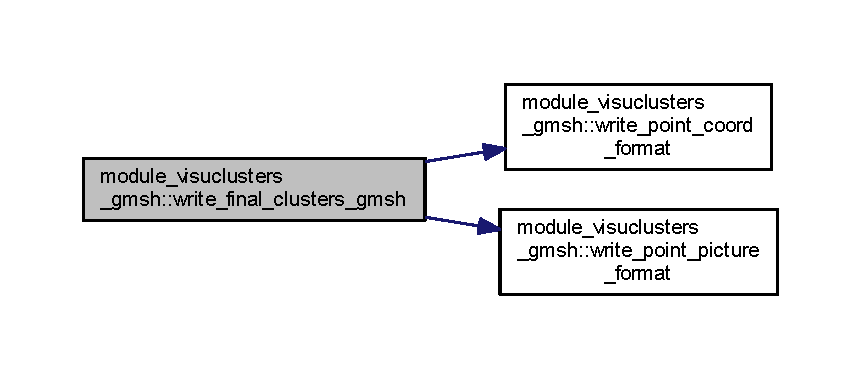
\includegraphics[width=350pt]{namespacemodule__visuclusters__gmsh_a3fe1790e0267b255e689ead80e6c8ca8_cgraph}
\end{center}
\end{figure}




Here is the caller graph for this function\+:\nopagebreak
\begin{figure}[H]
\begin{center}
\leavevmode
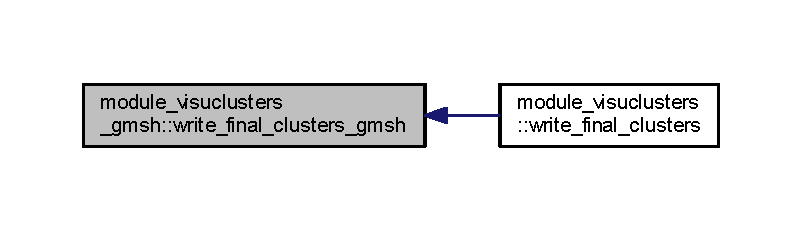
\includegraphics[width=350pt]{namespacemodule__visuclusters__gmsh_a3fe1790e0267b255e689ead80e6c8ca8_icgraph}
\end{center}
\end{figure}


\hypertarget{namespacemodule__visuclusters__gmsh_af04ca060cedb92fb755fd6cbb1330011}{}\index{module\+\_\+visuclusters\+\_\+gmsh@{module\+\_\+visuclusters\+\_\+gmsh}!write\+\_\+partial\+\_\+clusters\+\_\+gmsh@{write\+\_\+partial\+\_\+clusters\+\_\+gmsh}}
\index{write\+\_\+partial\+\_\+clusters\+\_\+gmsh@{write\+\_\+partial\+\_\+clusters\+\_\+gmsh}!module\+\_\+visuclusters\+\_\+gmsh@{module\+\_\+visuclusters\+\_\+gmsh}}
\subsubsection[{write\+\_\+partial\+\_\+clusters\+\_\+gmsh}]{\setlength{\rightskip}{0pt plus 5cm}subroutine module\+\_\+visuclusters\+\_\+gmsh\+::write\+\_\+partial\+\_\+clusters\+\_\+gmsh (
\begin{DoxyParamCaption}
\item[{type({\bf type\+\_\+params})}]{params}
\end{DoxyParamCaption}
)}\label{namespacemodule__visuclusters__gmsh_af04ca060cedb92fb755fd6cbb1330011}


Writes the clusters before grouping for Gmsh visualization. 

This methods extracts details on computed clusters on each domain from {\itshape cluster.\+partiel.\+x} files and writes them in corresponding {\itshape cluster.\+partiel.\+x.\+visu} files. \begin{DoxyNote}{Note}
{\itshape x} is the identifier (number) of a process. 
\end{DoxyNote}
\begin{DoxySeeAlso}{See also}
\hyperlink{namespacemodule__sortie_a24e663b5fc236eee7c6fe434493e342e}{module\+\_\+calcul\+::write\+\_\+partial\+\_\+clusters()} 
\end{DoxySeeAlso}

\begin{DoxyParams}[1]{Parameters}
\mbox{\tt in}  & {\em params} & the parameters defined in the \textit{param.in} file \\
\hline
\end{DoxyParams}


Here is the call graph for this function\+:\nopagebreak
\begin{figure}[H]
\begin{center}
\leavevmode
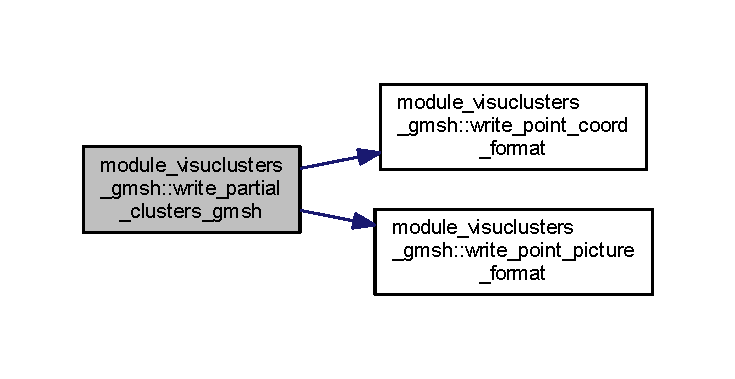
\includegraphics[width=350pt]{namespacemodule__visuclusters__gmsh_af04ca060cedb92fb755fd6cbb1330011_cgraph}
\end{center}
\end{figure}




Here is the caller graph for this function\+:\nopagebreak
\begin{figure}[H]
\begin{center}
\leavevmode
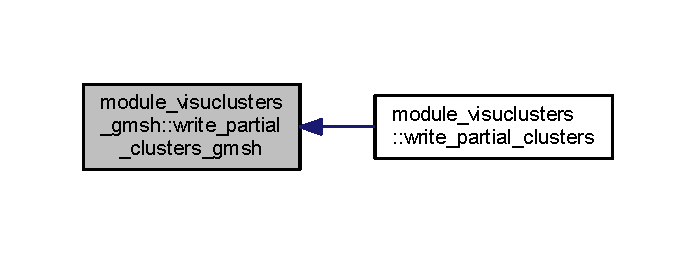
\includegraphics[width=334pt]{namespacemodule__visuclusters__gmsh_af04ca060cedb92fb755fd6cbb1330011_icgraph}
\end{center}
\end{figure}


\hypertarget{namespacemodule__visuclusters__gmsh_a2ffd04d2e2dcdda290446affaf3a76dc}{}\index{module\+\_\+visuclusters\+\_\+gmsh@{module\+\_\+visuclusters\+\_\+gmsh}!write\+\_\+partitioning\+\_\+gmsh@{write\+\_\+partitioning\+\_\+gmsh}}
\index{write\+\_\+partitioning\+\_\+gmsh@{write\+\_\+partitioning\+\_\+gmsh}!module\+\_\+visuclusters\+\_\+gmsh@{module\+\_\+visuclusters\+\_\+gmsh}}
\subsubsection[{write\+\_\+partitioning\+\_\+gmsh}]{\setlength{\rightskip}{0pt plus 5cm}subroutine module\+\_\+visuclusters\+\_\+gmsh\+::write\+\_\+partitioning\+\_\+gmsh (
\begin{DoxyParamCaption}
\item[{type({\bf type\+\_\+params})}]{params}
\end{DoxyParamCaption}
)}\label{namespacemodule__visuclusters__gmsh_a2ffd04d2e2dcdda290446affaf3a76dc}


Writes the geometry partitioning for Gmsh visualization. 

This methods extracts the domain definitions from the {\itshape fort.\+2} file and writes to {\itshape decoupe.\+geo} file, a source code file. We refer you to a \href{linkURL}{\tt Gmsh tutorial}. \begin{DoxySeeAlso}{See also}
\hyperlink{namespacemodule__sortie_abd1cdf529e5c71b3186c8d980e3d5117}{module\+\_\+calcul\+::write\+\_\+partitioning()} 
\end{DoxySeeAlso}

\begin{DoxyParams}[1]{Parameters}
\mbox{\tt in}  & {\em params} & the parameters defined in the \textit{param.in} file \\
\hline
\end{DoxyParams}


Here is the caller graph for this function\+:\nopagebreak
\begin{figure}[H]
\begin{center}
\leavevmode
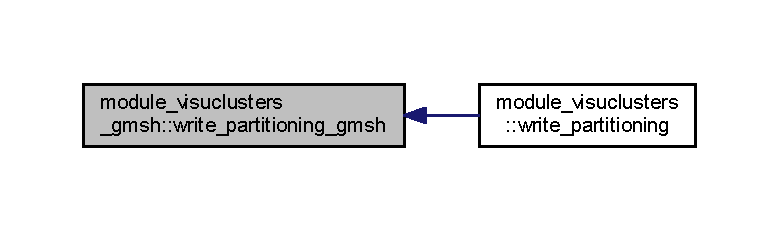
\includegraphics[width=350pt]{namespacemodule__visuclusters__gmsh_a2ffd04d2e2dcdda290446affaf3a76dc_icgraph}
\end{center}
\end{figure}


\hypertarget{namespacemodule__visuclusters__gmsh_ab3a87863baf4bd33953b9aa7950d5d26}{}\index{module\+\_\+visuclusters\+\_\+gmsh@{module\+\_\+visuclusters\+\_\+gmsh}!write\+\_\+point\+\_\+coord\+\_\+format@{write\+\_\+point\+\_\+coord\+\_\+format}}
\index{write\+\_\+point\+\_\+coord\+\_\+format@{write\+\_\+point\+\_\+coord\+\_\+format}!module\+\_\+visuclusters\+\_\+gmsh@{module\+\_\+visuclusters\+\_\+gmsh}}
\subsubsection[{write\+\_\+point\+\_\+coord\+\_\+format}]{\setlength{\rightskip}{0pt plus 5cm}subroutine module\+\_\+visuclusters\+\_\+gmsh\+::write\+\_\+point\+\_\+coord\+\_\+format (
\begin{DoxyParamCaption}
\item[{integer}]{unit, }
\item[{integer}]{dim, }
\item[{double precision, dimension(\+:,\+:), pointer}]{coords, }
\item[{integer}]{id, }
\item[{integer}]{k}
\end{DoxyParamCaption}
)}\label{namespacemodule__visuclusters__gmsh_ab3a87863baf4bd33953b9aa7950d5d26}


Writes point coordinates from coordinates format for Gmsh visualization. 



Here is the caller graph for this function\+:\nopagebreak
\begin{figure}[H]
\begin{center}
\leavevmode
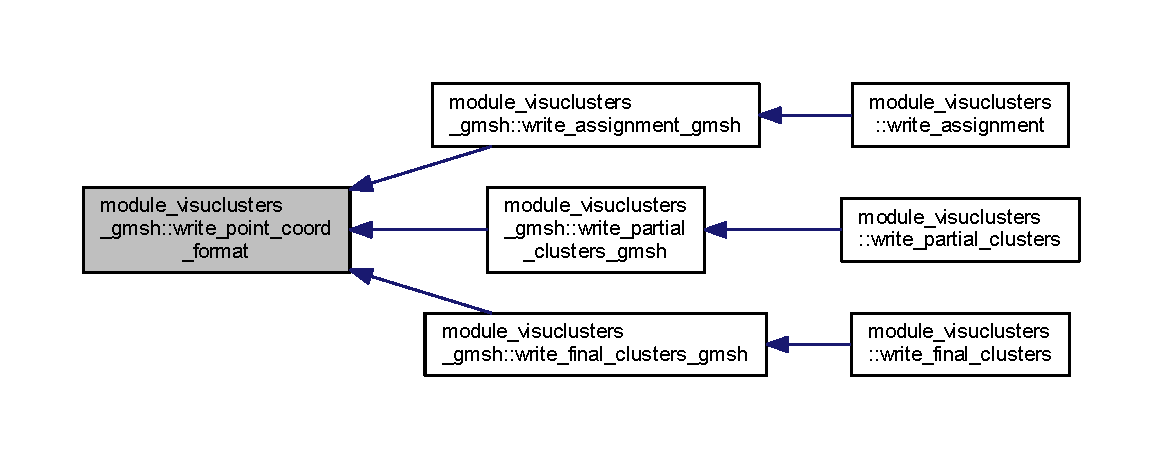
\includegraphics[width=350pt]{namespacemodule__visuclusters__gmsh_ab3a87863baf4bd33953b9aa7950d5d26_icgraph}
\end{center}
\end{figure}


\hypertarget{namespacemodule__visuclusters__gmsh_aa00f636e7ea0ae13557bdf9fa21b285f}{}\index{module\+\_\+visuclusters\+\_\+gmsh@{module\+\_\+visuclusters\+\_\+gmsh}!write\+\_\+point\+\_\+picture\+\_\+format@{write\+\_\+point\+\_\+picture\+\_\+format}}
\index{write\+\_\+point\+\_\+picture\+\_\+format@{write\+\_\+point\+\_\+picture\+\_\+format}!module\+\_\+visuclusters\+\_\+gmsh@{module\+\_\+visuclusters\+\_\+gmsh}}
\subsubsection[{write\+\_\+point\+\_\+picture\+\_\+format}]{\setlength{\rightskip}{0pt plus 5cm}subroutine module\+\_\+visuclusters\+\_\+gmsh\+::write\+\_\+point\+\_\+picture\+\_\+format (
\begin{DoxyParamCaption}
\item[{integer}]{unit, }
\item[{type({\bf type\+\_\+params})}]{params, }
\item[{integer}]{id, }
\item[{integer}]{k}
\end{DoxyParamCaption}
)}\label{namespacemodule__visuclusters__gmsh_aa00f636e7ea0ae13557bdf9fa21b285f}


Writes point coordinates from picture format for Gmsh visualization. 

The following is written in the file \+: 
\begin{DoxyEnumerate}
\item {\bfseries  For 2\+D case}\+: {\itshape  S\+P(x,y)\{id\} } 
\item {\bfseries  For 3\+D case}\+: {\itshape  S\+P(x,y,z)\{id\} } 
\end{DoxyEnumerate}\begin{DoxyNote}{Note}
x,y and z are the coordinates and id is the identifier of the process 
\end{DoxyNote}


Here is the caller graph for this function\+:\nopagebreak
\begin{figure}[H]
\begin{center}
\leavevmode
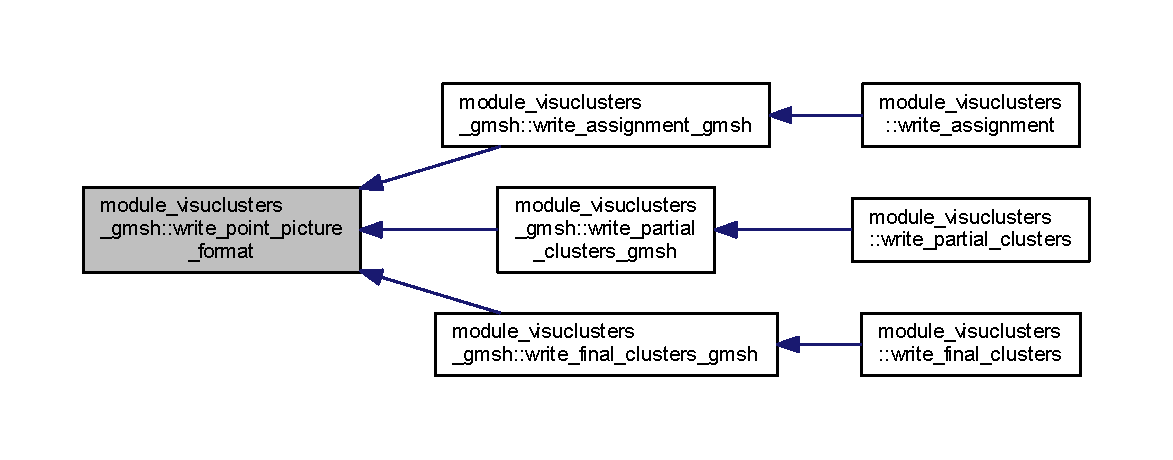
\includegraphics[width=350pt]{namespacemodule__visuclusters__gmsh_aa00f636e7ea0ae13557bdf9fa21b285f_icgraph}
\end{center}
\end{figure}



\hypertarget{namespacemodule__visuclusters__paraview}{}\section{module\+\_\+visuclusters\+\_\+paraview Module Reference}
\label{namespacemodule__visuclusters__paraview}\index{module\+\_\+visuclusters\+\_\+paraview@{module\+\_\+visuclusters\+\_\+paraview}}


Contains methods enabling writing results in file specifically formatted for Paraview.  


\subsection*{Functions/\+Subroutines}
\begin{DoxyCompactItemize}
\item 
subroutine \hyperlink{namespacemodule__visuclusters__paraview_a57010b34c7586dcf52fb9f50e2e1d7aa}{write\+\_\+partitioning\+\_\+paraview} (params)
\begin{DoxyCompactList}\small\item\em Writes the geometry partitioning for Paraview visualization. \end{DoxyCompactList}\item 
subroutine \hyperlink{namespacemodule__visuclusters__paraview_ad93eb4e679b429c757fcbf8831469a91}{write\+\_\+assignment\+\_\+paraview} (params)
\begin{DoxyCompactList}\small\item\em Initializes the file of the partitioning for Paraview visualization. \end{DoxyCompactList}\item 
subroutine \hyperlink{namespacemodule__visuclusters__paraview_abed87b4c957689d9cfdc62811f3b213b}{write\+\_\+partial\+\_\+clusters\+\_\+paraview} (params)
\begin{DoxyCompactList}\small\item\em Writes the clusters before grouping for Paraview visualization. \end{DoxyCompactList}\item 
subroutine \hyperlink{namespacemodule__visuclusters__paraview_a7e7514cf4abb2a7e0a8fa1d23252811e}{write\+\_\+final\+\_\+clusters\+\_\+paraview} (params)
\begin{DoxyCompactList}\small\item\em Writes the clusters after grouping for Paraview visualization. \end{DoxyCompactList}\item 
subroutine \hyperlink{namespacemodule__visuclusters__paraview_af62b5ff6548f1fd716d4931df4edeaf3}{write\+\_\+points\+\_\+coord\+\_\+format} (unit\+\_\+geo, unit\+\_\+ind, nb\+\_\+points, dim, coords, ids, k)
\begin{DoxyCompactList}\small\item\em Writes point coordinates from coordinates format for Paraview visualization. \end{DoxyCompactList}\item 
subroutine \hyperlink{namespacemodule__visuclusters__paraview_a532fbeef76809cf8c4ab2ea3cee9eaee}{write\+\_\+points\+\_\+picture\+\_\+format} (unit\+\_\+geo, unit\+\_\+ind, nb\+\_\+pixels, params, ids, proc\+\_\+ids)
\begin{DoxyCompactList}\small\item\em Writes point coordinates from picture format for Paraview visualization. \end{DoxyCompactList}\item 
subroutine \hyperlink{namespacemodule__visuclusters__paraview_a264164136b0ed4e82c5ef10cfaa2d649}{list\+\_\+commands\+\_\+paraview}
\begin{DoxyCompactList}\small\item\em Lists the commands related to Paraview visualization. \end{DoxyCompactList}\end{DoxyCompactItemize}


\subsection{Detailed Description}
Contains methods enabling writing results in file specifically formatted for Paraview. 

\subsection{Function/\+Subroutine Documentation}
\hypertarget{namespacemodule__visuclusters__paraview_a264164136b0ed4e82c5ef10cfaa2d649}{}\index{module\+\_\+visuclusters\+\_\+paraview@{module\+\_\+visuclusters\+\_\+paraview}!list\+\_\+commands\+\_\+paraview@{list\+\_\+commands\+\_\+paraview}}
\index{list\+\_\+commands\+\_\+paraview@{list\+\_\+commands\+\_\+paraview}!module\+\_\+visuclusters\+\_\+paraview@{module\+\_\+visuclusters\+\_\+paraview}}
\subsubsection[{list\+\_\+commands\+\_\+paraview}]{\setlength{\rightskip}{0pt plus 5cm}subroutine module\+\_\+visuclusters\+\_\+paraview\+::list\+\_\+commands\+\_\+paraview (
\begin{DoxyParamCaption}
{}
\end{DoxyParamCaption}
)}\label{namespacemodule__visuclusters__paraview_a264164136b0ed4e82c5ef10cfaa2d649}


Lists the commands related to Paraview visualization. 



Here is the caller graph for this function\+:\nopagebreak
\begin{figure}[H]
\begin{center}
\leavevmode
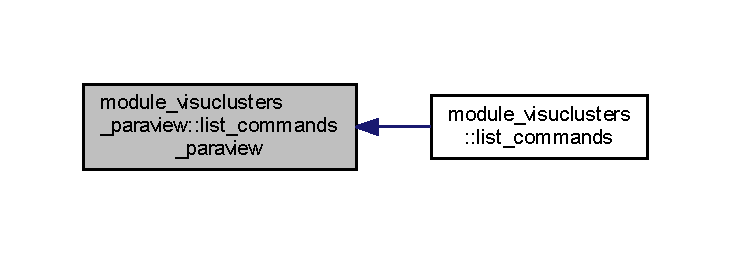
\includegraphics[width=350pt]{namespacemodule__visuclusters__paraview_a264164136b0ed4e82c5ef10cfaa2d649_icgraph}
\end{center}
\end{figure}


\hypertarget{namespacemodule__visuclusters__paraview_ad93eb4e679b429c757fcbf8831469a91}{}\index{module\+\_\+visuclusters\+\_\+paraview@{module\+\_\+visuclusters\+\_\+paraview}!write\+\_\+assignment\+\_\+paraview@{write\+\_\+assignment\+\_\+paraview}}
\index{write\+\_\+assignment\+\_\+paraview@{write\+\_\+assignment\+\_\+paraview}!module\+\_\+visuclusters\+\_\+paraview@{module\+\_\+visuclusters\+\_\+paraview}}
\subsubsection[{write\+\_\+assignment\+\_\+paraview}]{\setlength{\rightskip}{0pt plus 5cm}subroutine module\+\_\+visuclusters\+\_\+paraview\+::write\+\_\+assignment\+\_\+paraview (
\begin{DoxyParamCaption}
\item[{type({\bf type\+\_\+params})}]{params}
\end{DoxyParamCaption}
)}\label{namespacemodule__visuclusters__paraview_ad93eb4e679b429c757fcbf8831469a91}


Initializes the file of the partitioning for Paraview visualization. 

This method extracts details on partitioning from the {\itshape decoupe.\+x} files and writes them in {\itshape visu/affectation.$\ast$} files. Extra files are written in a case of interface partitioning. {\itshape visu/affectation-\/interface.$\ast$} files are the assignment for the interface. \begin{DoxyNote}{Note}
{\itshape x} is the identifier (number) of a process. 
\end{DoxyNote}
\begin{DoxySeeAlso}{See also}
\hyperlink{namespacemodule__sortie_abd1cdf529e5c71b3186c8d980e3d5117}{module\+\_\+calcul\+::write\+\_\+partitioning()}, \hyperlink{namespacemodule__decoupe_a523f2f851f39859d9c60114c934b2d66}{partition\+\_\+with\+\_\+interface()} 
\end{DoxySeeAlso}

\begin{DoxyParams}[1]{Parameters}
\mbox{\tt in}  & {\em params} & the parameters defined in the \textit{param.in} file \\
\hline
\end{DoxyParams}


Here is the call graph for this function\+:\nopagebreak
\begin{figure}[H]
\begin{center}
\leavevmode
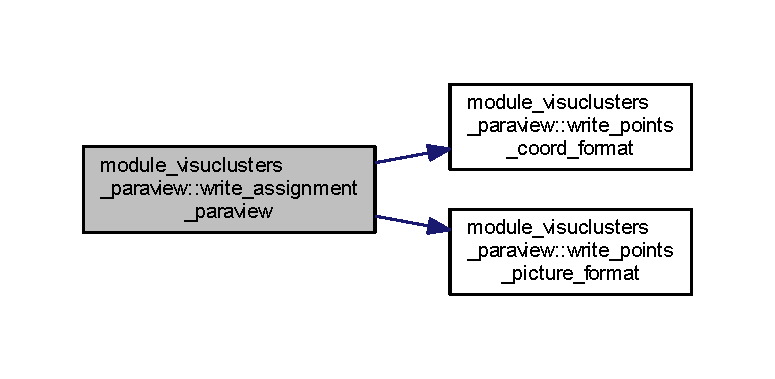
\includegraphics[width=350pt]{namespacemodule__visuclusters__paraview_ad93eb4e679b429c757fcbf8831469a91_cgraph}
\end{center}
\end{figure}




Here is the caller graph for this function\+:\nopagebreak
\begin{figure}[H]
\begin{center}
\leavevmode
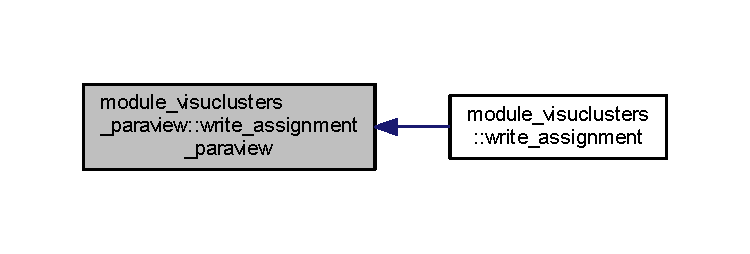
\includegraphics[width=350pt]{namespacemodule__visuclusters__paraview_ad93eb4e679b429c757fcbf8831469a91_icgraph}
\end{center}
\end{figure}


\hypertarget{namespacemodule__visuclusters__paraview_a7e7514cf4abb2a7e0a8fa1d23252811e}{}\index{module\+\_\+visuclusters\+\_\+paraview@{module\+\_\+visuclusters\+\_\+paraview}!write\+\_\+final\+\_\+clusters\+\_\+paraview@{write\+\_\+final\+\_\+clusters\+\_\+paraview}}
\index{write\+\_\+final\+\_\+clusters\+\_\+paraview@{write\+\_\+final\+\_\+clusters\+\_\+paraview}!module\+\_\+visuclusters\+\_\+paraview@{module\+\_\+visuclusters\+\_\+paraview}}
\subsubsection[{write\+\_\+final\+\_\+clusters\+\_\+paraview}]{\setlength{\rightskip}{0pt plus 5cm}subroutine module\+\_\+visuclusters\+\_\+paraview\+::write\+\_\+final\+\_\+clusters\+\_\+paraview (
\begin{DoxyParamCaption}
\item[{type({\bf type\+\_\+params})}]{params}
\end{DoxyParamCaption}
)}\label{namespacemodule__visuclusters__paraview_a7e7514cf4abb2a7e0a8fa1d23252811e}


Writes the clusters after grouping for Paraview visualization. 

This methods extracts details on computed clusters from {\itshape cluster.\+final.\+x} files and writes them in {\itshape cluster.\+final.\+visu} file. \begin{DoxyNote}{Note}
{\itshape x} is the identifier (number) of a cluster. 
\end{DoxyNote}
\begin{DoxySeeAlso}{See also}
\hyperlink{namespacemodule__sortie_a819ceed76e9600e8eec63a7b730d1d92}{module\+\_\+calcul\+::write\+\_\+final\+\_\+clusters()} 
\end{DoxySeeAlso}

\begin{DoxyParams}[1]{Parameters}
\mbox{\tt in}  & {\em params} & the parameters defined in the \textit{param.in} file \\
\hline
\end{DoxyParams}


Here is the call graph for this function\+:\nopagebreak
\begin{figure}[H]
\begin{center}
\leavevmode
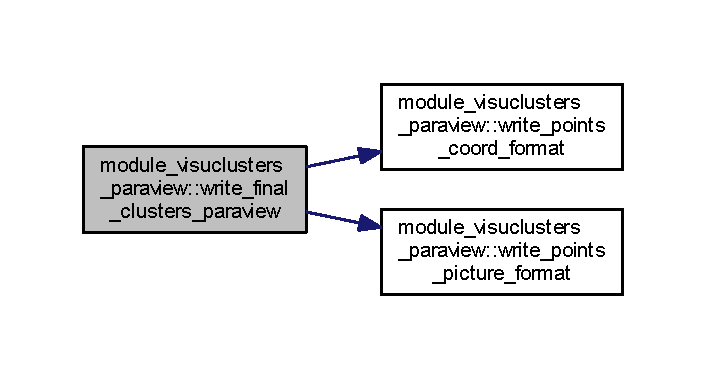
\includegraphics[width=339pt]{namespacemodule__visuclusters__paraview_a7e7514cf4abb2a7e0a8fa1d23252811e_cgraph}
\end{center}
\end{figure}




Here is the caller graph for this function\+:\nopagebreak
\begin{figure}[H]
\begin{center}
\leavevmode
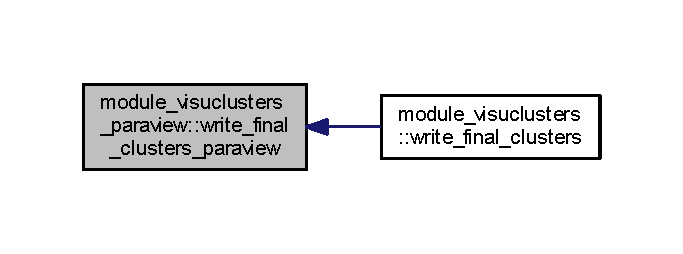
\includegraphics[width=328pt]{namespacemodule__visuclusters__paraview_a7e7514cf4abb2a7e0a8fa1d23252811e_icgraph}
\end{center}
\end{figure}


\hypertarget{namespacemodule__visuclusters__paraview_abed87b4c957689d9cfdc62811f3b213b}{}\index{module\+\_\+visuclusters\+\_\+paraview@{module\+\_\+visuclusters\+\_\+paraview}!write\+\_\+partial\+\_\+clusters\+\_\+paraview@{write\+\_\+partial\+\_\+clusters\+\_\+paraview}}
\index{write\+\_\+partial\+\_\+clusters\+\_\+paraview@{write\+\_\+partial\+\_\+clusters\+\_\+paraview}!module\+\_\+visuclusters\+\_\+paraview@{module\+\_\+visuclusters\+\_\+paraview}}
\subsubsection[{write\+\_\+partial\+\_\+clusters\+\_\+paraview}]{\setlength{\rightskip}{0pt plus 5cm}subroutine module\+\_\+visuclusters\+\_\+paraview\+::write\+\_\+partial\+\_\+clusters\+\_\+paraview (
\begin{DoxyParamCaption}
\item[{type({\bf type\+\_\+params})}]{params}
\end{DoxyParamCaption}
)}\label{namespacemodule__visuclusters__paraview_abed87b4c957689d9cfdc62811f3b213b}


Writes the clusters before grouping for Paraview visualization. 

This methods extracts details on computed clusters on each domain from {\itshape cluster.\+partiel.\+x} files and writes them in corresponding {\itshape visu/cluster.\+partiel.\+x.$\ast$} files. \begin{DoxyNote}{Note}
{\itshape x} is the identifier (number) of a process. 
\end{DoxyNote}
\begin{DoxySeeAlso}{See also}
\hyperlink{namespacemodule__sortie_a24e663b5fc236eee7c6fe434493e342e}{module\+\_\+calcul\+::write\+\_\+partial\+\_\+clusters()} 
\end{DoxySeeAlso}

\begin{DoxyParams}[1]{Parameters}
\mbox{\tt in}  & {\em params} & the parameters defined in the \textit{param.in} file \\
\hline
\end{DoxyParams}


Here is the call graph for this function\+:\nopagebreak
\begin{figure}[H]
\begin{center}
\leavevmode
\includegraphics[width=348pt]{namespacemodule__visuclusters__paraview_abed87b4c957689d9cfdc62811f3b213b_cgraph}
\end{center}
\end{figure}




Here is the caller graph for this function\+:\nopagebreak
\begin{figure}[H]
\begin{center}
\leavevmode
\includegraphics[width=346pt]{namespacemodule__visuclusters__paraview_abed87b4c957689d9cfdc62811f3b213b_icgraph}
\end{center}
\end{figure}


\hypertarget{namespacemodule__visuclusters__paraview_a57010b34c7586dcf52fb9f50e2e1d7aa}{}\index{module\+\_\+visuclusters\+\_\+paraview@{module\+\_\+visuclusters\+\_\+paraview}!write\+\_\+partitioning\+\_\+paraview@{write\+\_\+partitioning\+\_\+paraview}}
\index{write\+\_\+partitioning\+\_\+paraview@{write\+\_\+partitioning\+\_\+paraview}!module\+\_\+visuclusters\+\_\+paraview@{module\+\_\+visuclusters\+\_\+paraview}}
\subsubsection[{write\+\_\+partitioning\+\_\+paraview}]{\setlength{\rightskip}{0pt plus 5cm}subroutine module\+\_\+visuclusters\+\_\+paraview\+::write\+\_\+partitioning\+\_\+paraview (
\begin{DoxyParamCaption}
\item[{type({\bf type\+\_\+params})}]{params}
\end{DoxyParamCaption}
)}\label{namespacemodule__visuclusters__paraview_a57010b34c7586dcf52fb9f50e2e1d7aa}


Writes the geometry partitioning for Paraview visualization. 

This methods extracts the domain definitions from the {\itshape fort.\+2} file and writes to {\itshape visu/decoupe.$\ast$} files. \begin{DoxySeeAlso}{See also}
\hyperlink{namespacemodule__sortie_abd1cdf529e5c71b3186c8d980e3d5117}{module\+\_\+calcul\+::write\+\_\+partitioning()} 
\end{DoxySeeAlso}

\begin{DoxyParams}[1]{Parameters}
\mbox{\tt in}  & {\em params} & the parameters defined in the \textit{param.in} file \\
\hline
\end{DoxyParams}


Here is the caller graph for this function\+:\nopagebreak
\begin{figure}[H]
\begin{center}
\leavevmode
\includegraphics[width=350pt]{namespacemodule__visuclusters__paraview_a57010b34c7586dcf52fb9f50e2e1d7aa_icgraph}
\end{center}
\end{figure}


\hypertarget{namespacemodule__visuclusters__paraview_af62b5ff6548f1fd716d4931df4edeaf3}{}\index{module\+\_\+visuclusters\+\_\+paraview@{module\+\_\+visuclusters\+\_\+paraview}!write\+\_\+points\+\_\+coord\+\_\+format@{write\+\_\+points\+\_\+coord\+\_\+format}}
\index{write\+\_\+points\+\_\+coord\+\_\+format@{write\+\_\+points\+\_\+coord\+\_\+format}!module\+\_\+visuclusters\+\_\+paraview@{module\+\_\+visuclusters\+\_\+paraview}}
\subsubsection[{write\+\_\+points\+\_\+coord\+\_\+format}]{\setlength{\rightskip}{0pt plus 5cm}subroutine module\+\_\+visuclusters\+\_\+paraview\+::write\+\_\+points\+\_\+coord\+\_\+format (
\begin{DoxyParamCaption}
\item[{integer}]{unit\+\_\+geo, }
\item[{integer}]{unit\+\_\+ind, }
\item[{integer}]{nb\+\_\+points, }
\item[{integer}]{dim, }
\item[{double precision, dimension(\+:,\+:), pointer}]{coords, }
\item[{integer, dimension(\+:), pointer}]{ids, }
\item[{integer}]{k}
\end{DoxyParamCaption}
)}\label{namespacemodule__visuclusters__paraview_af62b5ff6548f1fd716d4931df4edeaf3}


Writes point coordinates from coordinates format for Paraview visualization. 



Here is the caller graph for this function\+:\nopagebreak
\begin{figure}[H]
\begin{center}
\leavevmode
\includegraphics[width=350pt]{namespacemodule__visuclusters__paraview_af62b5ff6548f1fd716d4931df4edeaf3_icgraph}
\end{center}
\end{figure}


\hypertarget{namespacemodule__visuclusters__paraview_a532fbeef76809cf8c4ab2ea3cee9eaee}{}\index{module\+\_\+visuclusters\+\_\+paraview@{module\+\_\+visuclusters\+\_\+paraview}!write\+\_\+points\+\_\+picture\+\_\+format@{write\+\_\+points\+\_\+picture\+\_\+format}}
\index{write\+\_\+points\+\_\+picture\+\_\+format@{write\+\_\+points\+\_\+picture\+\_\+format}!module\+\_\+visuclusters\+\_\+paraview@{module\+\_\+visuclusters\+\_\+paraview}}
\subsubsection[{write\+\_\+points\+\_\+picture\+\_\+format}]{\setlength{\rightskip}{0pt plus 5cm}subroutine module\+\_\+visuclusters\+\_\+paraview\+::write\+\_\+points\+\_\+picture\+\_\+format (
\begin{DoxyParamCaption}
\item[{integer}]{unit\+\_\+geo, }
\item[{integer}]{unit\+\_\+ind, }
\item[{integer}]{nb\+\_\+pixels, }
\item[{type({\bf type\+\_\+params})}]{params, }
\item[{integer, dimension(\+:), pointer}]{ids, }
\item[{integer, dimension(\+:), pointer}]{proc\+\_\+ids}
\end{DoxyParamCaption}
)}\label{namespacemodule__visuclusters__paraview_a532fbeef76809cf8c4ab2ea3cee9eaee}


Writes point coordinates from picture format for Paraview visualization. 

The following is written in the geometric file for each point \+: 
\begin{DoxyItemize}
\item {\bfseries  For 2\+D case}\+: {\itshape  x y } 
\item {\bfseries  For 3\+D case}\+: {\itshape  x y z} 
\end{DoxyItemize}And the following is written in the process partitioning file for each point \+: {\itshape  ind } \begin{DoxyNote}{Note}
x,y and z are the coordinates and ind is the identifier of the process. 

This method writes headers at first in the files. 
\end{DoxyNote}


Here is the caller graph for this function\+:\nopagebreak
\begin{figure}[H]
\begin{center}
\leavevmode
\includegraphics[width=350pt]{namespacemodule__visuclusters__paraview_a532fbeef76809cf8c4ab2ea3cee9eaee_icgraph}
\end{center}
\end{figure}



\hypertarget{namespacemodule__visuclusters__structure}{}\section{module\+\_\+visuclusters\+\_\+structure Module Reference}
\label{namespacemodule__visuclusters__structure}\index{module\+\_\+visuclusters\+\_\+structure@{module\+\_\+visuclusters\+\_\+structure}}


Contains useful data structures.  


\subsection*{Data Types}
\begin{DoxyCompactItemize}
\item 
type \hyperlink{structmodule__visuclusters__structure_1_1type__params}{type\+\_\+params}
\end{DoxyCompactItemize}


\subsection{Detailed Description}
Contains useful data structures. 
\chapter{Data Type Documentation}
\hypertarget{structmodule__structure_1_1type__clustering__param}{}\section{module\+\_\+structure\+:\+:type\+\_\+clustering\+\_\+param Type Reference}
\label{structmodule__structure_1_1type__clustering__param}\index{module\+\_\+structure\+::type\+\_\+clustering\+\_\+param@{module\+\_\+structure\+::type\+\_\+clustering\+\_\+param}}
\subsection*{Public Attributes}
\begin{DoxyCompactItemize}
\item 
integer \hyperlink{structmodule__structure_1_1type__clustering__param_a8bf29172007ac2bb0927ec135406618e}{clustering\+\_\+method\+\_\+id}
\item 
integer \hyperlink{structmodule__structure_1_1type__clustering__param_a1005f14a680a96a6b66bd82783d2153d}{kernelfunindex}
\item 
double precision \hyperlink{structmodule__structure_1_1type__clustering__param_a59a4870d2f3810136942a6f1ec116d0d}{sigma}
\item 
double precision \hyperlink{structmodule__structure_1_1type__clustering__param_ab899422852cb7f39a9dfeef2c3bed12f}{gam}
\item 
double precision \hyperlink{structmodule__structure_1_1type__clustering__param_a63047cf3dfca24f6c1647a1ee2b49f16}{delta}
\item 
integer \hyperlink{structmodule__structure_1_1type__clustering__param_ae401e511466a239a46f1a1233ba5b998}{bandwidth}
\end{DoxyCompactItemize}


\subsection{Member Data Documentation}
\hypertarget{structmodule__structure_1_1type__clustering__param_ae401e511466a239a46f1a1233ba5b998}{}\index{module\+\_\+structure\+::type\+\_\+clustering\+\_\+param@{module\+\_\+structure\+::type\+\_\+clustering\+\_\+param}!bandwidth@{bandwidth}}
\index{bandwidth@{bandwidth}!module\+\_\+structure\+::type\+\_\+clustering\+\_\+param@{module\+\_\+structure\+::type\+\_\+clustering\+\_\+param}}
\subsubsection[{bandwidth}]{\setlength{\rightskip}{0pt plus 5cm}integer module\+\_\+structure\+::type\+\_\+clustering\+\_\+param\+::bandwidth}\label{structmodule__structure_1_1type__clustering__param_ae401e511466a239a46f1a1233ba5b998}
\hypertarget{structmodule__structure_1_1type__clustering__param_a8bf29172007ac2bb0927ec135406618e}{}\index{module\+\_\+structure\+::type\+\_\+clustering\+\_\+param@{module\+\_\+structure\+::type\+\_\+clustering\+\_\+param}!clustering\+\_\+method\+\_\+id@{clustering\+\_\+method\+\_\+id}}
\index{clustering\+\_\+method\+\_\+id@{clustering\+\_\+method\+\_\+id}!module\+\_\+structure\+::type\+\_\+clustering\+\_\+param@{module\+\_\+structure\+::type\+\_\+clustering\+\_\+param}}
\subsubsection[{clustering\+\_\+method\+\_\+id}]{\setlength{\rightskip}{0pt plus 5cm}integer module\+\_\+structure\+::type\+\_\+clustering\+\_\+param\+::clustering\+\_\+method\+\_\+id}\label{structmodule__structure_1_1type__clustering__param_a8bf29172007ac2bb0927ec135406618e}
\hypertarget{structmodule__structure_1_1type__clustering__param_a63047cf3dfca24f6c1647a1ee2b49f16}{}\index{module\+\_\+structure\+::type\+\_\+clustering\+\_\+param@{module\+\_\+structure\+::type\+\_\+clustering\+\_\+param}!delta@{delta}}
\index{delta@{delta}!module\+\_\+structure\+::type\+\_\+clustering\+\_\+param@{module\+\_\+structure\+::type\+\_\+clustering\+\_\+param}}
\subsubsection[{delta}]{\setlength{\rightskip}{0pt plus 5cm}double precision module\+\_\+structure\+::type\+\_\+clustering\+\_\+param\+::delta}\label{structmodule__structure_1_1type__clustering__param_a63047cf3dfca24f6c1647a1ee2b49f16}
\hypertarget{structmodule__structure_1_1type__clustering__param_ab899422852cb7f39a9dfeef2c3bed12f}{}\index{module\+\_\+structure\+::type\+\_\+clustering\+\_\+param@{module\+\_\+structure\+::type\+\_\+clustering\+\_\+param}!gam@{gam}}
\index{gam@{gam}!module\+\_\+structure\+::type\+\_\+clustering\+\_\+param@{module\+\_\+structure\+::type\+\_\+clustering\+\_\+param}}
\subsubsection[{gam}]{\setlength{\rightskip}{0pt plus 5cm}double precision module\+\_\+structure\+::type\+\_\+clustering\+\_\+param\+::gam}\label{structmodule__structure_1_1type__clustering__param_ab899422852cb7f39a9dfeef2c3bed12f}
\hypertarget{structmodule__structure_1_1type__clustering__param_a1005f14a680a96a6b66bd82783d2153d}{}\index{module\+\_\+structure\+::type\+\_\+clustering\+\_\+param@{module\+\_\+structure\+::type\+\_\+clustering\+\_\+param}!kernelfunindex@{kernelfunindex}}
\index{kernelfunindex@{kernelfunindex}!module\+\_\+structure\+::type\+\_\+clustering\+\_\+param@{module\+\_\+structure\+::type\+\_\+clustering\+\_\+param}}
\subsubsection[{kernelfunindex}]{\setlength{\rightskip}{0pt plus 5cm}integer module\+\_\+structure\+::type\+\_\+clustering\+\_\+param\+::kernelfunindex}\label{structmodule__structure_1_1type__clustering__param_a1005f14a680a96a6b66bd82783d2153d}
\hypertarget{structmodule__structure_1_1type__clustering__param_a59a4870d2f3810136942a6f1ec116d0d}{}\index{module\+\_\+structure\+::type\+\_\+clustering\+\_\+param@{module\+\_\+structure\+::type\+\_\+clustering\+\_\+param}!sigma@{sigma}}
\index{sigma@{sigma}!module\+\_\+structure\+::type\+\_\+clustering\+\_\+param@{module\+\_\+structure\+::type\+\_\+clustering\+\_\+param}}
\subsubsection[{sigma}]{\setlength{\rightskip}{0pt plus 5cm}double precision module\+\_\+structure\+::type\+\_\+clustering\+\_\+param\+::sigma}\label{structmodule__structure_1_1type__clustering__param_a59a4870d2f3810136942a6f1ec116d0d}

\hypertarget{structmodule__structure_1_1type__clusters}{}\section{module\+\_\+structure\+:\+:type\+\_\+clusters Type Reference}
\label{structmodule__structure_1_1type__clusters}\index{module\+\_\+structure\+::type\+\_\+clusters@{module\+\_\+structure\+::type\+\_\+clusters}}
\subsection*{Public Attributes}
\begin{DoxyCompactItemize}
\item 
integer, dimension(\+:), pointer \hyperlink{structmodule__structure_1_1type__clusters_a3b74e396e16d1393351f1e618377d5d3}{nbelt}
\item 
integer \hyperlink{structmodule__structure_1_1type__clusters_a64434771f896188453c607f24aa6246d}{nb}
\end{DoxyCompactItemize}


\subsection{Member Data Documentation}
\hypertarget{structmodule__structure_1_1type__clusters_a64434771f896188453c607f24aa6246d}{}\index{module\+\_\+structure\+::type\+\_\+clusters@{module\+\_\+structure\+::type\+\_\+clusters}!nb@{nb}}
\index{nb@{nb}!module\+\_\+structure\+::type\+\_\+clusters@{module\+\_\+structure\+::type\+\_\+clusters}}
\subsubsection[{nb}]{\setlength{\rightskip}{0pt plus 5cm}integer module\+\_\+structure\+::type\+\_\+clusters\+::nb}\label{structmodule__structure_1_1type__clusters_a64434771f896188453c607f24aa6246d}
\hypertarget{structmodule__structure_1_1type__clusters_a3b74e396e16d1393351f1e618377d5d3}{}\index{module\+\_\+structure\+::type\+\_\+clusters@{module\+\_\+structure\+::type\+\_\+clusters}!nbelt@{nbelt}}
\index{nbelt@{nbelt}!module\+\_\+structure\+::type\+\_\+clusters@{module\+\_\+structure\+::type\+\_\+clusters}}
\subsubsection[{nbelt}]{\setlength{\rightskip}{0pt plus 5cm}integer, dimension(\+:), pointer module\+\_\+structure\+::type\+\_\+clusters\+::nbelt}\label{structmodule__structure_1_1type__clusters_a3b74e396e16d1393351f1e618377d5d3}

\hypertarget{structmodule__structure_1_1type__data}{}\section{module\+\_\+structure\+:\+:type\+\_\+data Type Reference}
\label{structmodule__structure_1_1type__data}\index{module\+\_\+structure\+::type\+\_\+data@{module\+\_\+structure\+::type\+\_\+data}}


Collaboration diagram for module\+\_\+structure\+:\+:type\+\_\+data\+:\nopagebreak
\begin{figure}[H]
\begin{center}
\leavevmode
\includegraphics[width=220pt]{structmodule__structure_1_1type__data__coll__graph}
\end{center}
\end{figure}
\subsection*{Public Attributes}
\begin{DoxyCompactItemize}
\item 
type(\hyperlink{structmodule__structure_1_1type__points}{type\+\_\+points}), dimension(\+:), pointer \hyperlink{structmodule__structure_1_1type__data_abf37f99fee0c2349e30eeb7154a83781}{point}
\item 
integer \hyperlink{structmodule__structure_1_1type__data_aeda213b55a528437b4c0c62419c7ea16}{nb}
\item 
integer \hyperlink{structmodule__structure_1_1type__data_a34f9035cfb1ea16372e037570762092b}{dim}
\item 
integer \hyperlink{structmodule__structure_1_1type__data_a4d92879e85d1d01490acc4dfcd2cb919}{nbclusters}
\item 
integer \hyperlink{structmodule__structure_1_1type__data_ac7205be3a73581de07ce87c73512e053}{coord}
\item 
integer \hyperlink{structmodule__structure_1_1type__data_ad94fb30180d08b822535fe3871a6f8e5}{image}
\item 
integer \hyperlink{structmodule__structure_1_1type__data_aea3be74c0bedcbf99fcdb1667557f0f7}{geom}
\item 
integer \hyperlink{structmodule__structure_1_1type__data_a3ee52c32703411f359fba32fc811dafb}{seuil}
\item 
integer \hyperlink{structmodule__structure_1_1type__data_a96f87a53c6f8260511e272eae3890b14}{interface}
\item 
integer \hyperlink{structmodule__structure_1_1type__data_a48f072d67251fec80f72a58076491ca7}{recouvrement}
\item 
double precision, dimension(\+:), pointer \hyperlink{structmodule__structure_1_1type__data_ac7bbaf17e7397368148e848611d34244}{pas}
\item 
integer, dimension(\+:,\+:), pointer \hyperlink{structmodule__structure_1_1type__data_acb77a7774d04786633bf0ef6482a5d00}{refimg}
\item 
integer, dimension(\+:), pointer \hyperlink{structmodule__structure_1_1type__data_a923214c4f0d6d624a16e2320cf461093}{imgmap}
\item 
integer \hyperlink{structmodule__structure_1_1type__data_ae1e79afbe614fabb6bcc79837f40b75f}{imgdim}
\item 
integer \hyperlink{structmodule__structure_1_1type__data_a55743cf7c72081de117e4160110ed553}{imgt}
\end{DoxyCompactItemize}


\subsection{Member Data Documentation}
\hypertarget{structmodule__structure_1_1type__data_ac7205be3a73581de07ce87c73512e053}{}\index{module\+\_\+structure\+::type\+\_\+data@{module\+\_\+structure\+::type\+\_\+data}!coord@{coord}}
\index{coord@{coord}!module\+\_\+structure\+::type\+\_\+data@{module\+\_\+structure\+::type\+\_\+data}}
\subsubsection[{coord}]{\setlength{\rightskip}{0pt plus 5cm}integer module\+\_\+structure\+::type\+\_\+data\+::coord}\label{structmodule__structure_1_1type__data_ac7205be3a73581de07ce87c73512e053}
\hypertarget{structmodule__structure_1_1type__data_a34f9035cfb1ea16372e037570762092b}{}\index{module\+\_\+structure\+::type\+\_\+data@{module\+\_\+structure\+::type\+\_\+data}!dim@{dim}}
\index{dim@{dim}!module\+\_\+structure\+::type\+\_\+data@{module\+\_\+structure\+::type\+\_\+data}}
\subsubsection[{dim}]{\setlength{\rightskip}{0pt plus 5cm}integer module\+\_\+structure\+::type\+\_\+data\+::dim}\label{structmodule__structure_1_1type__data_a34f9035cfb1ea16372e037570762092b}
\hypertarget{structmodule__structure_1_1type__data_aea3be74c0bedcbf99fcdb1667557f0f7}{}\index{module\+\_\+structure\+::type\+\_\+data@{module\+\_\+structure\+::type\+\_\+data}!geom@{geom}}
\index{geom@{geom}!module\+\_\+structure\+::type\+\_\+data@{module\+\_\+structure\+::type\+\_\+data}}
\subsubsection[{geom}]{\setlength{\rightskip}{0pt plus 5cm}integer module\+\_\+structure\+::type\+\_\+data\+::geom}\label{structmodule__structure_1_1type__data_aea3be74c0bedcbf99fcdb1667557f0f7}
\hypertarget{structmodule__structure_1_1type__data_ad94fb30180d08b822535fe3871a6f8e5}{}\index{module\+\_\+structure\+::type\+\_\+data@{module\+\_\+structure\+::type\+\_\+data}!image@{image}}
\index{image@{image}!module\+\_\+structure\+::type\+\_\+data@{module\+\_\+structure\+::type\+\_\+data}}
\subsubsection[{image}]{\setlength{\rightskip}{0pt plus 5cm}integer module\+\_\+structure\+::type\+\_\+data\+::image}\label{structmodule__structure_1_1type__data_ad94fb30180d08b822535fe3871a6f8e5}
\hypertarget{structmodule__structure_1_1type__data_ae1e79afbe614fabb6bcc79837f40b75f}{}\index{module\+\_\+structure\+::type\+\_\+data@{module\+\_\+structure\+::type\+\_\+data}!imgdim@{imgdim}}
\index{imgdim@{imgdim}!module\+\_\+structure\+::type\+\_\+data@{module\+\_\+structure\+::type\+\_\+data}}
\subsubsection[{imgdim}]{\setlength{\rightskip}{0pt plus 5cm}integer module\+\_\+structure\+::type\+\_\+data\+::imgdim}\label{structmodule__structure_1_1type__data_ae1e79afbe614fabb6bcc79837f40b75f}
\hypertarget{structmodule__structure_1_1type__data_a923214c4f0d6d624a16e2320cf461093}{}\index{module\+\_\+structure\+::type\+\_\+data@{module\+\_\+structure\+::type\+\_\+data}!imgmap@{imgmap}}
\index{imgmap@{imgmap}!module\+\_\+structure\+::type\+\_\+data@{module\+\_\+structure\+::type\+\_\+data}}
\subsubsection[{imgmap}]{\setlength{\rightskip}{0pt plus 5cm}integer, dimension(\+:), pointer module\+\_\+structure\+::type\+\_\+data\+::imgmap}\label{structmodule__structure_1_1type__data_a923214c4f0d6d624a16e2320cf461093}
\hypertarget{structmodule__structure_1_1type__data_a55743cf7c72081de117e4160110ed553}{}\index{module\+\_\+structure\+::type\+\_\+data@{module\+\_\+structure\+::type\+\_\+data}!imgt@{imgt}}
\index{imgt@{imgt}!module\+\_\+structure\+::type\+\_\+data@{module\+\_\+structure\+::type\+\_\+data}}
\subsubsection[{imgt}]{\setlength{\rightskip}{0pt plus 5cm}integer module\+\_\+structure\+::type\+\_\+data\+::imgt}\label{structmodule__structure_1_1type__data_a55743cf7c72081de117e4160110ed553}
\hypertarget{structmodule__structure_1_1type__data_a96f87a53c6f8260511e272eae3890b14}{}\index{module\+\_\+structure\+::type\+\_\+data@{module\+\_\+structure\+::type\+\_\+data}!interface@{interface}}
\index{interface@{interface}!module\+\_\+structure\+::type\+\_\+data@{module\+\_\+structure\+::type\+\_\+data}}
\subsubsection[{interface}]{\setlength{\rightskip}{0pt plus 5cm}integer module\+\_\+structure\+::type\+\_\+data\+::interface}\label{structmodule__structure_1_1type__data_a96f87a53c6f8260511e272eae3890b14}
\hypertarget{structmodule__structure_1_1type__data_aeda213b55a528437b4c0c62419c7ea16}{}\index{module\+\_\+structure\+::type\+\_\+data@{module\+\_\+structure\+::type\+\_\+data}!nb@{nb}}
\index{nb@{nb}!module\+\_\+structure\+::type\+\_\+data@{module\+\_\+structure\+::type\+\_\+data}}
\subsubsection[{nb}]{\setlength{\rightskip}{0pt plus 5cm}integer module\+\_\+structure\+::type\+\_\+data\+::nb}\label{structmodule__structure_1_1type__data_aeda213b55a528437b4c0c62419c7ea16}
\hypertarget{structmodule__structure_1_1type__data_a4d92879e85d1d01490acc4dfcd2cb919}{}\index{module\+\_\+structure\+::type\+\_\+data@{module\+\_\+structure\+::type\+\_\+data}!nbclusters@{nbclusters}}
\index{nbclusters@{nbclusters}!module\+\_\+structure\+::type\+\_\+data@{module\+\_\+structure\+::type\+\_\+data}}
\subsubsection[{nbclusters}]{\setlength{\rightskip}{0pt plus 5cm}integer module\+\_\+structure\+::type\+\_\+data\+::nbclusters}\label{structmodule__structure_1_1type__data_a4d92879e85d1d01490acc4dfcd2cb919}
\hypertarget{structmodule__structure_1_1type__data_ac7bbaf17e7397368148e848611d34244}{}\index{module\+\_\+structure\+::type\+\_\+data@{module\+\_\+structure\+::type\+\_\+data}!pas@{pas}}
\index{pas@{pas}!module\+\_\+structure\+::type\+\_\+data@{module\+\_\+structure\+::type\+\_\+data}}
\subsubsection[{pas}]{\setlength{\rightskip}{0pt plus 5cm}double precision, dimension(\+:), pointer module\+\_\+structure\+::type\+\_\+data\+::pas}\label{structmodule__structure_1_1type__data_ac7bbaf17e7397368148e848611d34244}
\hypertarget{structmodule__structure_1_1type__data_abf37f99fee0c2349e30eeb7154a83781}{}\index{module\+\_\+structure\+::type\+\_\+data@{module\+\_\+structure\+::type\+\_\+data}!point@{point}}
\index{point@{point}!module\+\_\+structure\+::type\+\_\+data@{module\+\_\+structure\+::type\+\_\+data}}
\subsubsection[{point}]{\setlength{\rightskip}{0pt plus 5cm}type({\bf type\+\_\+points}), dimension(\+:), pointer module\+\_\+structure\+::type\+\_\+data\+::point}\label{structmodule__structure_1_1type__data_abf37f99fee0c2349e30eeb7154a83781}
\hypertarget{structmodule__structure_1_1type__data_a48f072d67251fec80f72a58076491ca7}{}\index{module\+\_\+structure\+::type\+\_\+data@{module\+\_\+structure\+::type\+\_\+data}!recouvrement@{recouvrement}}
\index{recouvrement@{recouvrement}!module\+\_\+structure\+::type\+\_\+data@{module\+\_\+structure\+::type\+\_\+data}}
\subsubsection[{recouvrement}]{\setlength{\rightskip}{0pt plus 5cm}integer module\+\_\+structure\+::type\+\_\+data\+::recouvrement}\label{structmodule__structure_1_1type__data_a48f072d67251fec80f72a58076491ca7}
\hypertarget{structmodule__structure_1_1type__data_acb77a7774d04786633bf0ef6482a5d00}{}\index{module\+\_\+structure\+::type\+\_\+data@{module\+\_\+structure\+::type\+\_\+data}!refimg@{refimg}}
\index{refimg@{refimg}!module\+\_\+structure\+::type\+\_\+data@{module\+\_\+structure\+::type\+\_\+data}}
\subsubsection[{refimg}]{\setlength{\rightskip}{0pt plus 5cm}integer, dimension(\+:,\+:), pointer module\+\_\+structure\+::type\+\_\+data\+::refimg}\label{structmodule__structure_1_1type__data_acb77a7774d04786633bf0ef6482a5d00}
\hypertarget{structmodule__structure_1_1type__data_a3ee52c32703411f359fba32fc811dafb}{}\index{module\+\_\+structure\+::type\+\_\+data@{module\+\_\+structure\+::type\+\_\+data}!seuil@{seuil}}
\index{seuil@{seuil}!module\+\_\+structure\+::type\+\_\+data@{module\+\_\+structure\+::type\+\_\+data}}
\subsubsection[{seuil}]{\setlength{\rightskip}{0pt plus 5cm}integer module\+\_\+structure\+::type\+\_\+data\+::seuil}\label{structmodule__structure_1_1type__data_a3ee52c32703411f359fba32fc811dafb}

\hypertarget{structmodule__visuclusters__structure_1_1type__params}{}\section{module\+\_\+visuclusters\+\_\+structure\+:\+:type\+\_\+params Type Reference}
\label{structmodule__visuclusters__structure_1_1type__params}\index{module\+\_\+visuclusters\+\_\+structure\+::type\+\_\+params@{module\+\_\+visuclusters\+\_\+structure\+::type\+\_\+params}}
\subsection*{Public Attributes}
\begin{DoxyCompactItemize}
\item 
character(len=30) \hyperlink{structmodule__visuclusters__structure_1_1type__params_a2217cf949d7c0691fa70b7a654d9db20}{mesh}
\item 
double precision, dimension(\+:), pointer \hyperlink{structmodule__visuclusters__structure_1_1type__params_a400a0deb3ac4ced38bae01ccbe6148f0}{pas}
\item 
integer, dimension(\+:,\+:), pointer \hyperlink{structmodule__visuclusters__structure_1_1type__params_aac8aed43c2a6498a0cda0fa76a29615a}{refimg}
\item 
integer, dimension(\+:), pointer \hyperlink{structmodule__visuclusters__structure_1_1type__params_ab1cdbb95c62b0edbbb81025b93353421}{imgmap}
\item 
integer \hyperlink{structmodule__visuclusters__structure_1_1type__params_a34c16c92c7d1386a2044ce3600ce1c49}{coord}
\item 
integer \hyperlink{structmodule__visuclusters__structure_1_1type__params_a3362eae2ef386fcab58bc168e673b227}{dim}
\item 
integer \hyperlink{structmodule__visuclusters__structure_1_1type__params_a893bedbfe22fca04b088bd7f001ed963}{geom}
\item 
integer \hyperlink{structmodule__visuclusters__structure_1_1type__params_af36709484754bb4577400fb4bcf44ab7}{image}
\item 
integer \hyperlink{structmodule__visuclusters__structure_1_1type__params_abc632497fd004d3dc7d8f0428e532587}{imgdim}
\item 
integer \hyperlink{structmodule__visuclusters__structure_1_1type__params_a12024c5bfa94e5fad4d0110fa603d090}{imgt}
\item 
integer \hyperlink{structmodule__visuclusters__structure_1_1type__params_ae57b6a715225b9e6c0a22a22580b8905}{interface}
\item 
integer \hyperlink{structmodule__visuclusters__structure_1_1type__params_ad24a003143b6a72be056d77eae9a2757}{nbclusters}
\item 
integer \hyperlink{structmodule__visuclusters__structure_1_1type__params_a8b78bd72af8bdabd21acfd6f2314e6dc}{nbp}
\item 
integer \hyperlink{structmodule__visuclusters__structure_1_1type__params_a6b5bc9580c4cc5ddac09f70e87b9affe}{nbproc}
\item 
integer \hyperlink{structmodule__visuclusters__structure_1_1type__params_aeefa371e1a8a47cb214715ae2e67627f}{recouvrement}
\item 
integer \hyperlink{structmodule__visuclusters__structure_1_1type__params_a3cd977202ff5db7cd0db292d654aa68f}{seuil}
\end{DoxyCompactItemize}


\subsection{Member Data Documentation}
\hypertarget{structmodule__visuclusters__structure_1_1type__params_a34c16c92c7d1386a2044ce3600ce1c49}{}\index{module\+\_\+visuclusters\+\_\+structure\+::type\+\_\+params@{module\+\_\+visuclusters\+\_\+structure\+::type\+\_\+params}!coord@{coord}}
\index{coord@{coord}!module\+\_\+visuclusters\+\_\+structure\+::type\+\_\+params@{module\+\_\+visuclusters\+\_\+structure\+::type\+\_\+params}}
\subsubsection[{coord}]{\setlength{\rightskip}{0pt plus 5cm}integer module\+\_\+visuclusters\+\_\+structure\+::type\+\_\+params\+::coord}\label{structmodule__visuclusters__structure_1_1type__params_a34c16c92c7d1386a2044ce3600ce1c49}
\hypertarget{structmodule__visuclusters__structure_1_1type__params_a3362eae2ef386fcab58bc168e673b227}{}\index{module\+\_\+visuclusters\+\_\+structure\+::type\+\_\+params@{module\+\_\+visuclusters\+\_\+structure\+::type\+\_\+params}!dim@{dim}}
\index{dim@{dim}!module\+\_\+visuclusters\+\_\+structure\+::type\+\_\+params@{module\+\_\+visuclusters\+\_\+structure\+::type\+\_\+params}}
\subsubsection[{dim}]{\setlength{\rightskip}{0pt plus 5cm}integer module\+\_\+visuclusters\+\_\+structure\+::type\+\_\+params\+::dim}\label{structmodule__visuclusters__structure_1_1type__params_a3362eae2ef386fcab58bc168e673b227}
\hypertarget{structmodule__visuclusters__structure_1_1type__params_a893bedbfe22fca04b088bd7f001ed963}{}\index{module\+\_\+visuclusters\+\_\+structure\+::type\+\_\+params@{module\+\_\+visuclusters\+\_\+structure\+::type\+\_\+params}!geom@{geom}}
\index{geom@{geom}!module\+\_\+visuclusters\+\_\+structure\+::type\+\_\+params@{module\+\_\+visuclusters\+\_\+structure\+::type\+\_\+params}}
\subsubsection[{geom}]{\setlength{\rightskip}{0pt plus 5cm}integer module\+\_\+visuclusters\+\_\+structure\+::type\+\_\+params\+::geom}\label{structmodule__visuclusters__structure_1_1type__params_a893bedbfe22fca04b088bd7f001ed963}
\hypertarget{structmodule__visuclusters__structure_1_1type__params_af36709484754bb4577400fb4bcf44ab7}{}\index{module\+\_\+visuclusters\+\_\+structure\+::type\+\_\+params@{module\+\_\+visuclusters\+\_\+structure\+::type\+\_\+params}!image@{image}}
\index{image@{image}!module\+\_\+visuclusters\+\_\+structure\+::type\+\_\+params@{module\+\_\+visuclusters\+\_\+structure\+::type\+\_\+params}}
\subsubsection[{image}]{\setlength{\rightskip}{0pt plus 5cm}integer module\+\_\+visuclusters\+\_\+structure\+::type\+\_\+params\+::image}\label{structmodule__visuclusters__structure_1_1type__params_af36709484754bb4577400fb4bcf44ab7}
\hypertarget{structmodule__visuclusters__structure_1_1type__params_abc632497fd004d3dc7d8f0428e532587}{}\index{module\+\_\+visuclusters\+\_\+structure\+::type\+\_\+params@{module\+\_\+visuclusters\+\_\+structure\+::type\+\_\+params}!imgdim@{imgdim}}
\index{imgdim@{imgdim}!module\+\_\+visuclusters\+\_\+structure\+::type\+\_\+params@{module\+\_\+visuclusters\+\_\+structure\+::type\+\_\+params}}
\subsubsection[{imgdim}]{\setlength{\rightskip}{0pt plus 5cm}integer module\+\_\+visuclusters\+\_\+structure\+::type\+\_\+params\+::imgdim}\label{structmodule__visuclusters__structure_1_1type__params_abc632497fd004d3dc7d8f0428e532587}
\hypertarget{structmodule__visuclusters__structure_1_1type__params_ab1cdbb95c62b0edbbb81025b93353421}{}\index{module\+\_\+visuclusters\+\_\+structure\+::type\+\_\+params@{module\+\_\+visuclusters\+\_\+structure\+::type\+\_\+params}!imgmap@{imgmap}}
\index{imgmap@{imgmap}!module\+\_\+visuclusters\+\_\+structure\+::type\+\_\+params@{module\+\_\+visuclusters\+\_\+structure\+::type\+\_\+params}}
\subsubsection[{imgmap}]{\setlength{\rightskip}{0pt plus 5cm}integer, dimension(\+:), pointer module\+\_\+visuclusters\+\_\+structure\+::type\+\_\+params\+::imgmap}\label{structmodule__visuclusters__structure_1_1type__params_ab1cdbb95c62b0edbbb81025b93353421}
\hypertarget{structmodule__visuclusters__structure_1_1type__params_a12024c5bfa94e5fad4d0110fa603d090}{}\index{module\+\_\+visuclusters\+\_\+structure\+::type\+\_\+params@{module\+\_\+visuclusters\+\_\+structure\+::type\+\_\+params}!imgt@{imgt}}
\index{imgt@{imgt}!module\+\_\+visuclusters\+\_\+structure\+::type\+\_\+params@{module\+\_\+visuclusters\+\_\+structure\+::type\+\_\+params}}
\subsubsection[{imgt}]{\setlength{\rightskip}{0pt plus 5cm}integer module\+\_\+visuclusters\+\_\+structure\+::type\+\_\+params\+::imgt}\label{structmodule__visuclusters__structure_1_1type__params_a12024c5bfa94e5fad4d0110fa603d090}
\hypertarget{structmodule__visuclusters__structure_1_1type__params_ae57b6a715225b9e6c0a22a22580b8905}{}\index{module\+\_\+visuclusters\+\_\+structure\+::type\+\_\+params@{module\+\_\+visuclusters\+\_\+structure\+::type\+\_\+params}!interface@{interface}}
\index{interface@{interface}!module\+\_\+visuclusters\+\_\+structure\+::type\+\_\+params@{module\+\_\+visuclusters\+\_\+structure\+::type\+\_\+params}}
\subsubsection[{interface}]{\setlength{\rightskip}{0pt plus 5cm}integer module\+\_\+visuclusters\+\_\+structure\+::type\+\_\+params\+::interface}\label{structmodule__visuclusters__structure_1_1type__params_ae57b6a715225b9e6c0a22a22580b8905}
\hypertarget{structmodule__visuclusters__structure_1_1type__params_a2217cf949d7c0691fa70b7a654d9db20}{}\index{module\+\_\+visuclusters\+\_\+structure\+::type\+\_\+params@{module\+\_\+visuclusters\+\_\+structure\+::type\+\_\+params}!mesh@{mesh}}
\index{mesh@{mesh}!module\+\_\+visuclusters\+\_\+structure\+::type\+\_\+params@{module\+\_\+visuclusters\+\_\+structure\+::type\+\_\+params}}
\subsubsection[{mesh}]{\setlength{\rightskip}{0pt plus 5cm}character (len=30) module\+\_\+visuclusters\+\_\+structure\+::type\+\_\+params\+::mesh}\label{structmodule__visuclusters__structure_1_1type__params_a2217cf949d7c0691fa70b7a654d9db20}
\hypertarget{structmodule__visuclusters__structure_1_1type__params_ad24a003143b6a72be056d77eae9a2757}{}\index{module\+\_\+visuclusters\+\_\+structure\+::type\+\_\+params@{module\+\_\+visuclusters\+\_\+structure\+::type\+\_\+params}!nbclusters@{nbclusters}}
\index{nbclusters@{nbclusters}!module\+\_\+visuclusters\+\_\+structure\+::type\+\_\+params@{module\+\_\+visuclusters\+\_\+structure\+::type\+\_\+params}}
\subsubsection[{nbclusters}]{\setlength{\rightskip}{0pt plus 5cm}integer module\+\_\+visuclusters\+\_\+structure\+::type\+\_\+params\+::nbclusters}\label{structmodule__visuclusters__structure_1_1type__params_ad24a003143b6a72be056d77eae9a2757}
\hypertarget{structmodule__visuclusters__structure_1_1type__params_a8b78bd72af8bdabd21acfd6f2314e6dc}{}\index{module\+\_\+visuclusters\+\_\+structure\+::type\+\_\+params@{module\+\_\+visuclusters\+\_\+structure\+::type\+\_\+params}!nbp@{nbp}}
\index{nbp@{nbp}!module\+\_\+visuclusters\+\_\+structure\+::type\+\_\+params@{module\+\_\+visuclusters\+\_\+structure\+::type\+\_\+params}}
\subsubsection[{nbp}]{\setlength{\rightskip}{0pt plus 5cm}integer module\+\_\+visuclusters\+\_\+structure\+::type\+\_\+params\+::nbp}\label{structmodule__visuclusters__structure_1_1type__params_a8b78bd72af8bdabd21acfd6f2314e6dc}
\hypertarget{structmodule__visuclusters__structure_1_1type__params_a6b5bc9580c4cc5ddac09f70e87b9affe}{}\index{module\+\_\+visuclusters\+\_\+structure\+::type\+\_\+params@{module\+\_\+visuclusters\+\_\+structure\+::type\+\_\+params}!nbproc@{nbproc}}
\index{nbproc@{nbproc}!module\+\_\+visuclusters\+\_\+structure\+::type\+\_\+params@{module\+\_\+visuclusters\+\_\+structure\+::type\+\_\+params}}
\subsubsection[{nbproc}]{\setlength{\rightskip}{0pt plus 5cm}integer module\+\_\+visuclusters\+\_\+structure\+::type\+\_\+params\+::nbproc}\label{structmodule__visuclusters__structure_1_1type__params_a6b5bc9580c4cc5ddac09f70e87b9affe}
\hypertarget{structmodule__visuclusters__structure_1_1type__params_a400a0deb3ac4ced38bae01ccbe6148f0}{}\index{module\+\_\+visuclusters\+\_\+structure\+::type\+\_\+params@{module\+\_\+visuclusters\+\_\+structure\+::type\+\_\+params}!pas@{pas}}
\index{pas@{pas}!module\+\_\+visuclusters\+\_\+structure\+::type\+\_\+params@{module\+\_\+visuclusters\+\_\+structure\+::type\+\_\+params}}
\subsubsection[{pas}]{\setlength{\rightskip}{0pt plus 5cm}double precision, dimension(\+:), pointer module\+\_\+visuclusters\+\_\+structure\+::type\+\_\+params\+::pas}\label{structmodule__visuclusters__structure_1_1type__params_a400a0deb3ac4ced38bae01ccbe6148f0}
\hypertarget{structmodule__visuclusters__structure_1_1type__params_aeefa371e1a8a47cb214715ae2e67627f}{}\index{module\+\_\+visuclusters\+\_\+structure\+::type\+\_\+params@{module\+\_\+visuclusters\+\_\+structure\+::type\+\_\+params}!recouvrement@{recouvrement}}
\index{recouvrement@{recouvrement}!module\+\_\+visuclusters\+\_\+structure\+::type\+\_\+params@{module\+\_\+visuclusters\+\_\+structure\+::type\+\_\+params}}
\subsubsection[{recouvrement}]{\setlength{\rightskip}{0pt plus 5cm}integer module\+\_\+visuclusters\+\_\+structure\+::type\+\_\+params\+::recouvrement}\label{structmodule__visuclusters__structure_1_1type__params_aeefa371e1a8a47cb214715ae2e67627f}
\hypertarget{structmodule__visuclusters__structure_1_1type__params_aac8aed43c2a6498a0cda0fa76a29615a}{}\index{module\+\_\+visuclusters\+\_\+structure\+::type\+\_\+params@{module\+\_\+visuclusters\+\_\+structure\+::type\+\_\+params}!refimg@{refimg}}
\index{refimg@{refimg}!module\+\_\+visuclusters\+\_\+structure\+::type\+\_\+params@{module\+\_\+visuclusters\+\_\+structure\+::type\+\_\+params}}
\subsubsection[{refimg}]{\setlength{\rightskip}{0pt plus 5cm}integer, dimension(\+:,\+:), pointer module\+\_\+visuclusters\+\_\+structure\+::type\+\_\+params\+::refimg}\label{structmodule__visuclusters__structure_1_1type__params_aac8aed43c2a6498a0cda0fa76a29615a}
\hypertarget{structmodule__visuclusters__structure_1_1type__params_a3cd977202ff5db7cd0db292d654aa68f}{}\index{module\+\_\+visuclusters\+\_\+structure\+::type\+\_\+params@{module\+\_\+visuclusters\+\_\+structure\+::type\+\_\+params}!seuil@{seuil}}
\index{seuil@{seuil}!module\+\_\+visuclusters\+\_\+structure\+::type\+\_\+params@{module\+\_\+visuclusters\+\_\+structure\+::type\+\_\+params}}
\subsubsection[{seuil}]{\setlength{\rightskip}{0pt plus 5cm}integer module\+\_\+visuclusters\+\_\+structure\+::type\+\_\+params\+::seuil}\label{structmodule__visuclusters__structure_1_1type__params_a3cd977202ff5db7cd0db292d654aa68f}

\hypertarget{structmodule__structure_1_1type__points}{}\section{module\+\_\+structure\+:\+:type\+\_\+points Type Reference}
\label{structmodule__structure_1_1type__points}\index{module\+\_\+structure\+::type\+\_\+points@{module\+\_\+structure\+::type\+\_\+points}}
\subsection*{Public Attributes}
\begin{DoxyCompactItemize}
\item 
double precision, dimension(\+:), pointer \hyperlink{structmodule__structure_1_1type__points_a81d059927ede51f531d5ac3e97bb654c}{coord}
\item 
integer \hyperlink{structmodule__structure_1_1type__points_a04dcced1bb30414993dc5e2d9546ef61}{cluster}
\end{DoxyCompactItemize}


\subsection{Member Data Documentation}
\hypertarget{structmodule__structure_1_1type__points_a04dcced1bb30414993dc5e2d9546ef61}{}\index{module\+\_\+structure\+::type\+\_\+points@{module\+\_\+structure\+::type\+\_\+points}!cluster@{cluster}}
\index{cluster@{cluster}!module\+\_\+structure\+::type\+\_\+points@{module\+\_\+structure\+::type\+\_\+points}}
\subsubsection[{cluster}]{\setlength{\rightskip}{0pt plus 5cm}integer module\+\_\+structure\+::type\+\_\+points\+::cluster}\label{structmodule__structure_1_1type__points_a04dcced1bb30414993dc5e2d9546ef61}
\hypertarget{structmodule__structure_1_1type__points_a81d059927ede51f531d5ac3e97bb654c}{}\index{module\+\_\+structure\+::type\+\_\+points@{module\+\_\+structure\+::type\+\_\+points}!coord@{coord}}
\index{coord@{coord}!module\+\_\+structure\+::type\+\_\+points@{module\+\_\+structure\+::type\+\_\+points}}
\subsubsection[{coord}]{\setlength{\rightskip}{0pt plus 5cm}double precision, dimension(\+:), pointer module\+\_\+structure\+::type\+\_\+points\+::coord}\label{structmodule__structure_1_1type__points_a81d059927ede51f531d5ac3e97bb654c}

\hypertarget{structmodule__teste__clusters_1_1type__test}{}\section{module\+\_\+teste\+\_\+clusters\+:\+:type\+\_\+test Type Reference}
\label{structmodule__teste__clusters_1_1type__test}\index{module\+\_\+teste\+\_\+clusters\+::type\+\_\+test@{module\+\_\+teste\+\_\+clusters\+::type\+\_\+test}}
\subsection*{Public Attributes}
\begin{DoxyCompactItemize}
\item 
character(len=80) \hyperlink{structmodule__teste__clusters_1_1type__test_a8b4d3aabaaea5f2881a91b6001928989}{datatype}
\item 
character(len=80) \hyperlink{structmodule__teste__clusters_1_1type__test_abf7078230df53518aa75cf4c0e883230}{decoupetype}
\item 
character(len=80) \hyperlink{structmodule__teste__clusters_1_1type__test_a3f0c9892ac12f878cef715596063b6a0}{dir}
\item 
character(len=80) \hyperlink{structmodule__teste__clusters_1_1type__test_a75ab1290d6885c0563d6756975f8f9c8}{fichier}
\item 
character(len=80) \hyperlink{structmodule__teste__clusters_1_1type__test_a00b4f0f089f7fa8ecccc6d8bd84cf927}{output}
\item 
character(len=80) \hyperlink{structmodule__teste__clusters_1_1type__test_a4f64d7525145220b6e3e94580d2033dc}{visup}
\item 
character(len=80) \hyperlink{structmodule__teste__clusters_1_1type__test_a44e54c0ee5ae01a2234a6b9e6d7758b6}{visug}
\item 
double precision \hyperlink{structmodule__teste__clusters_1_1type__test_a39ba4beaad65966bff6fd0b3897bf0bc}{epaisseur}
\item 
integer, dimension(\+:), pointer \hyperlink{structmodule__teste__clusters_1_1type__test_a1eceed0de4bd5829751ba0a32b2d2eb4}{decoupe}
\item 
integer \hyperlink{structmodule__teste__clusters_1_1type__test_aecd0c97ab0c069345644bcf354bb7842}{nbproc}
\end{DoxyCompactItemize}


\subsection{Member Data Documentation}
\hypertarget{structmodule__teste__clusters_1_1type__test_a8b4d3aabaaea5f2881a91b6001928989}{}\index{module\+\_\+teste\+\_\+clusters\+::type\+\_\+test@{module\+\_\+teste\+\_\+clusters\+::type\+\_\+test}!datatype@{datatype}}
\index{datatype@{datatype}!module\+\_\+teste\+\_\+clusters\+::type\+\_\+test@{module\+\_\+teste\+\_\+clusters\+::type\+\_\+test}}
\subsubsection[{datatype}]{\setlength{\rightskip}{0pt plus 5cm}character (len=80) module\+\_\+teste\+\_\+clusters\+::type\+\_\+test\+::datatype}\label{structmodule__teste__clusters_1_1type__test_a8b4d3aabaaea5f2881a91b6001928989}
\hypertarget{structmodule__teste__clusters_1_1type__test_a1eceed0de4bd5829751ba0a32b2d2eb4}{}\index{module\+\_\+teste\+\_\+clusters\+::type\+\_\+test@{module\+\_\+teste\+\_\+clusters\+::type\+\_\+test}!decoupe@{decoupe}}
\index{decoupe@{decoupe}!module\+\_\+teste\+\_\+clusters\+::type\+\_\+test@{module\+\_\+teste\+\_\+clusters\+::type\+\_\+test}}
\subsubsection[{decoupe}]{\setlength{\rightskip}{0pt plus 5cm}integer, dimension(\+:), pointer module\+\_\+teste\+\_\+clusters\+::type\+\_\+test\+::decoupe}\label{structmodule__teste__clusters_1_1type__test_a1eceed0de4bd5829751ba0a32b2d2eb4}
\hypertarget{structmodule__teste__clusters_1_1type__test_abf7078230df53518aa75cf4c0e883230}{}\index{module\+\_\+teste\+\_\+clusters\+::type\+\_\+test@{module\+\_\+teste\+\_\+clusters\+::type\+\_\+test}!decoupetype@{decoupetype}}
\index{decoupetype@{decoupetype}!module\+\_\+teste\+\_\+clusters\+::type\+\_\+test@{module\+\_\+teste\+\_\+clusters\+::type\+\_\+test}}
\subsubsection[{decoupetype}]{\setlength{\rightskip}{0pt plus 5cm}character (len=80) module\+\_\+teste\+\_\+clusters\+::type\+\_\+test\+::decoupetype}\label{structmodule__teste__clusters_1_1type__test_abf7078230df53518aa75cf4c0e883230}
\hypertarget{structmodule__teste__clusters_1_1type__test_a3f0c9892ac12f878cef715596063b6a0}{}\index{module\+\_\+teste\+\_\+clusters\+::type\+\_\+test@{module\+\_\+teste\+\_\+clusters\+::type\+\_\+test}!dir@{dir}}
\index{dir@{dir}!module\+\_\+teste\+\_\+clusters\+::type\+\_\+test@{module\+\_\+teste\+\_\+clusters\+::type\+\_\+test}}
\subsubsection[{dir}]{\setlength{\rightskip}{0pt plus 5cm}character (len=80) module\+\_\+teste\+\_\+clusters\+::type\+\_\+test\+::dir}\label{structmodule__teste__clusters_1_1type__test_a3f0c9892ac12f878cef715596063b6a0}
\hypertarget{structmodule__teste__clusters_1_1type__test_a39ba4beaad65966bff6fd0b3897bf0bc}{}\index{module\+\_\+teste\+\_\+clusters\+::type\+\_\+test@{module\+\_\+teste\+\_\+clusters\+::type\+\_\+test}!epaisseur@{epaisseur}}
\index{epaisseur@{epaisseur}!module\+\_\+teste\+\_\+clusters\+::type\+\_\+test@{module\+\_\+teste\+\_\+clusters\+::type\+\_\+test}}
\subsubsection[{epaisseur}]{\setlength{\rightskip}{0pt plus 5cm}double precision module\+\_\+teste\+\_\+clusters\+::type\+\_\+test\+::epaisseur}\label{structmodule__teste__clusters_1_1type__test_a39ba4beaad65966bff6fd0b3897bf0bc}
\hypertarget{structmodule__teste__clusters_1_1type__test_a75ab1290d6885c0563d6756975f8f9c8}{}\index{module\+\_\+teste\+\_\+clusters\+::type\+\_\+test@{module\+\_\+teste\+\_\+clusters\+::type\+\_\+test}!fichier@{fichier}}
\index{fichier@{fichier}!module\+\_\+teste\+\_\+clusters\+::type\+\_\+test@{module\+\_\+teste\+\_\+clusters\+::type\+\_\+test}}
\subsubsection[{fichier}]{\setlength{\rightskip}{0pt plus 5cm}character (len=80) module\+\_\+teste\+\_\+clusters\+::type\+\_\+test\+::fichier}\label{structmodule__teste__clusters_1_1type__test_a75ab1290d6885c0563d6756975f8f9c8}
\hypertarget{structmodule__teste__clusters_1_1type__test_aecd0c97ab0c069345644bcf354bb7842}{}\index{module\+\_\+teste\+\_\+clusters\+::type\+\_\+test@{module\+\_\+teste\+\_\+clusters\+::type\+\_\+test}!nbproc@{nbproc}}
\index{nbproc@{nbproc}!module\+\_\+teste\+\_\+clusters\+::type\+\_\+test@{module\+\_\+teste\+\_\+clusters\+::type\+\_\+test}}
\subsubsection[{nbproc}]{\setlength{\rightskip}{0pt plus 5cm}integer module\+\_\+teste\+\_\+clusters\+::type\+\_\+test\+::nbproc}\label{structmodule__teste__clusters_1_1type__test_aecd0c97ab0c069345644bcf354bb7842}
\hypertarget{structmodule__teste__clusters_1_1type__test_a00b4f0f089f7fa8ecccc6d8bd84cf927}{}\index{module\+\_\+teste\+\_\+clusters\+::type\+\_\+test@{module\+\_\+teste\+\_\+clusters\+::type\+\_\+test}!output@{output}}
\index{output@{output}!module\+\_\+teste\+\_\+clusters\+::type\+\_\+test@{module\+\_\+teste\+\_\+clusters\+::type\+\_\+test}}
\subsubsection[{output}]{\setlength{\rightskip}{0pt plus 5cm}character (len=80) module\+\_\+teste\+\_\+clusters\+::type\+\_\+test\+::output}\label{structmodule__teste__clusters_1_1type__test_a00b4f0f089f7fa8ecccc6d8bd84cf927}
\hypertarget{structmodule__teste__clusters_1_1type__test_a44e54c0ee5ae01a2234a6b9e6d7758b6}{}\index{module\+\_\+teste\+\_\+clusters\+::type\+\_\+test@{module\+\_\+teste\+\_\+clusters\+::type\+\_\+test}!visug@{visug}}
\index{visug@{visug}!module\+\_\+teste\+\_\+clusters\+::type\+\_\+test@{module\+\_\+teste\+\_\+clusters\+::type\+\_\+test}}
\subsubsection[{visug}]{\setlength{\rightskip}{0pt plus 5cm}character (len=80) module\+\_\+teste\+\_\+clusters\+::type\+\_\+test\+::visug}\label{structmodule__teste__clusters_1_1type__test_a44e54c0ee5ae01a2234a6b9e6d7758b6}
\hypertarget{structmodule__teste__clusters_1_1type__test_a4f64d7525145220b6e3e94580d2033dc}{}\index{module\+\_\+teste\+\_\+clusters\+::type\+\_\+test@{module\+\_\+teste\+\_\+clusters\+::type\+\_\+test}!visup@{visup}}
\index{visup@{visup}!module\+\_\+teste\+\_\+clusters\+::type\+\_\+test@{module\+\_\+teste\+\_\+clusters\+::type\+\_\+test}}
\subsubsection[{visup}]{\setlength{\rightskip}{0pt plus 5cm}character (len=80) module\+\_\+teste\+\_\+clusters\+::type\+\_\+test\+::visup}\label{structmodule__teste__clusters_1_1type__test_a4f64d7525145220b6e3e94580d2033dc}

\chapter{File Documentation}
\hypertarget{module__calcul_8f90}{}\section{module\+\_\+calcul.\+f90 File Reference}
\label{module__calcul_8f90}\index{module\+\_\+calcul.\+f90@{module\+\_\+calcul.\+f90}}
\subsection*{Modules}
\begin{DoxyCompactItemize}
\item 
module \hyperlink{namespacemodule__calcul}{module\+\_\+calcul}
\begin{DoxyCompactList}\small\item\em Contains the spectral clustering method and methods that computes affinity parameters for kernels and overlapping. \end{DoxyCompactList}\end{DoxyCompactItemize}
\subsection*{Functions/\+Subroutines}
\begin{DoxyCompactItemize}
\item 
subroutine \hyperlink{namespacemodule__calcul_abd05b2b3ee81b4f779744a951d8a4c05}{module\+\_\+calcul\+::get\+\_\+sigma} (partitioned\+\_\+data, sigma)
\begin{DoxyCompactList}\small\item\em Computes the affinity parameter $sigma$. \end{DoxyCompactList}\item 
subroutine \hyperlink{namespacemodule__calcul_a118fd6a58b1064989fa68460457bea60}{module\+\_\+calcul\+::get\+\_\+sigma\+\_\+interface} (proc\+\_\+id, partitioned\+\_\+data, sigma, bounds, partitioning, epsilon)
\begin{DoxyCompactList}\small\item\em Computes the affinity parameter $sigma$ for the interface. \end{DoxyCompactList}\item 
double precision function, dimension(partitioned\+\_\+data\%nb, partitioned\+\_\+data\%nb) \hyperlink{namespacemodule__calcul_a97fd8d0653adb9041ab3ca899c0d0f91}{module\+\_\+calcul\+::poly\+\_\+kernel} (partitioned\+\_\+data, gam, delta)
\item 
double precision function, dimension(partitioned\+\_\+data\%nb, partitioned\+\_\+data\%nb) \hyperlink{namespacemodule__calcul_a44b26b54d1b94dddba0ba575be04658b}{module\+\_\+calcul\+::gaussian\+\_\+kernel} (partitioned\+\_\+data, sigma)
\item 
subroutine \hyperlink{namespacemodule__calcul_a72848eb89fbd2fe4a97512f53752ca5c}{module\+\_\+calcul\+::apply\+\_\+kernel\+\_\+k\+\_\+means} (proc\+\_\+id, nb\+\_\+clusters\+\_\+max, nb\+\_\+clusters\+\_\+opt, partitioned\+\_\+data, clust\+\_\+param)
\item 
subroutine \hyperlink{namespacemodule__calcul_a7bf1a318c636b4e204f267103d00114a}{module\+\_\+calcul\+::apply\+\_\+spectral\+\_\+clustering} (proc\+\_\+id, nb\+\_\+clusters\+\_\+max, nb\+\_\+clusters\+\_\+opt, partitioned\+\_\+data, sigma, clust\+\_\+param)
\item 
subroutine \hyperlink{namespacemodule__calcul_abb4a64b9f338e54274a250b9c10bf0bd}{module\+\_\+calcul\+::mean\+\_\+shift} (proc\+\_\+id, nb\+\_\+clusters\+\_\+max, nb\+\_\+clusters\+\_\+opt, partitioned\+\_\+data, bandwidth)
\end{DoxyCompactItemize}

\hypertarget{module__decoupe_8f90}{}\section{module\+\_\+decoupe.\+f90 File Reference}
\label{module__decoupe_8f90}\index{module\+\_\+decoupe.\+f90@{module\+\_\+decoupe.\+f90}}
\subsection*{Modules}
\begin{DoxyCompactItemize}
\item 
module \hyperlink{namespacemodule__decoupe}{module\+\_\+decoupe}
\begin{DoxyCompactList}\small\item\em Contains methods enabling the partitionning and the groupping of the data. \end{DoxyCompactList}\end{DoxyCompactItemize}
\subsection*{Functions/\+Subroutines}
\begin{DoxyCompactItemize}
\item 
subroutine \hyperlink{namespacemodule__decoupe_a20e9d554b6d62aa1aac7be71c223132e}{module\+\_\+decoupe\+::partition\+\_\+data} (data, epsilon, nb\+\_\+proc, coord\+\_\+min, coord\+\_\+max, partitioning, points\+\_\+by\+\_\+domain, assignements, bounds)
\begin{DoxyCompactList}\small\item\em Partitions the data into subdomains for a latter processing by the slaves. \end{DoxyCompactList}\item 
subroutine \hyperlink{namespacemodule__decoupe_ab1bd43de3891732cdf5803c4d86544dd}{module\+\_\+decoupe\+::define\+\_\+bounds} (data, coord\+\_\+min, coord\+\_\+max, bounds, partitioning, epsilon, nb\+\_\+proc)
\begin{DoxyCompactList}\small\item\em Defines the bounds of each subdomain. \end{DoxyCompactList}\item 
subroutine \hyperlink{namespacemodule__decoupe_afc4d3c1d1e2c287779200be5cf9d8205}{module\+\_\+decoupe\+::define\+\_\+domains} (nb\+\_\+proc, data, domains, bounds, partitioning)
\begin{DoxyCompactList}\small\item\em Defines the different subdomains. \end{DoxyCompactList}\item 
subroutine \hyperlink{namespacemodule__decoupe_a523f2f851f39859d9c60114c934b2d66}{module\+\_\+decoupe\+::partition\+\_\+with\+\_\+interface} (nb\+\_\+proc, data, points\+\_\+by\+\_\+domain, assignements, domains, epsilon)
\begin{DoxyCompactList}\small\item\em Partitions the data using interface. \end{DoxyCompactList}\item 
subroutine \hyperlink{namespacemodule__decoupe_a6f29dcc8367ffa44fa720260882fa04e}{module\+\_\+decoupe\+::partition\+\_\+with\+\_\+overlapping} (nb\+\_\+proc, data, points\+\_\+by\+\_\+domain, assignements, domains)
\begin{DoxyCompactList}\small\item\em Partitions the data using overlapping. \end{DoxyCompactList}\item 
subroutine \hyperlink{namespacemodule__decoupe_af5369423cd2f8c975e68cbc08c7b31c1}{module\+\_\+decoupe\+::group\+\_\+clusters} (nb\+\_\+clusters, points\+\_\+by\+\_\+cluster, cluster\+\_\+map, data)
\begin{DoxyCompactList}\small\item\em Groups the clusters and removes duplicates from the set of found clusters. \end{DoxyCompactList}\end{DoxyCompactItemize}

\hypertarget{module__embed_8f90}{}\section{module\+\_\+embed.\+f90 File Reference}
\label{module__embed_8f90}\index{module\+\_\+embed.\+f90@{module\+\_\+embed.\+f90}}
\subsection*{Modules}
\begin{DoxyCompactItemize}
\item 
module \hyperlink{namespacemodule__embed}{module\+\_\+embed}
\begin{DoxyCompactList}\small\item\em Contains K-\/means and spectral embedding algorithms. \end{DoxyCompactList}\end{DoxyCompactItemize}
\subsection*{Functions/\+Subroutines}
\begin{DoxyCompactItemize}
\item 
subroutine \hyperlink{namespacemodule__embed_ab78350f96b04d0ce2ca0bd10abd50440}{module\+\_\+embed\+::apply\+\_\+spectral\+\_\+embedding} (nb\+\_\+clusters, n, Z, A, ratio, clusters, clusters\+\_\+centers, points\+\_\+by\+\_\+clusters, clusters\+\_\+energies, nb\+\_\+info, proc\+\_\+id, ratio\+\_\+moy, ratio\+\_\+rij, ratio\+\_\+rii)
\begin{DoxyCompactList}\small\item\em Computes the clusters using eigen vector matrix. \end{DoxyCompactList}\item 
subroutine \hyperlink{namespacemodule__embed_a27f0555abee781e67c2def5e2b9471d2}{module\+\_\+embed\+::apply\+\_\+kmeans} (dim, nb\+\_\+points, nb\+\_\+clusters, nb\+\_\+iter\+\_\+max, nb\+\_\+iter, points, clusters, clusters\+\_\+centers, points\+\_\+by\+\_\+clusters, clusters\+\_\+energies, proc\+\_\+id)
\begin{DoxyCompactList}\small\item\em Implements K-\/\+Means algorithm (required by spectral clustering and Kernel K-\/\+Means methods) The algorithm works as follows\+: \end{DoxyCompactList}\end{DoxyCompactItemize}

\hypertarget{module__entree_8f90}{}\section{module\+\_\+entree.\+f90 File Reference}
\label{module__entree_8f90}\index{module\+\_\+entree.\+f90@{module\+\_\+entree.\+f90}}
\subsection*{Modules}
\begin{DoxyCompactItemize}
\item 
module \hyperlink{namespacemodule__entree}{module\+\_\+entree}
\begin{DoxyCompactList}\small\item\em Contains methods enabling data and parameter file reading. \end{DoxyCompactList}\end{DoxyCompactItemize}
\subsection*{Functions/\+Subroutines}
\begin{DoxyCompactItemize}
\item 
subroutine \hyperlink{namespacemodule__entree_ae91fc1d896afb27c01d7314dce81db70}{module\+\_\+entree\+::help}
\begin{DoxyCompactList}\small\item\em Displays help on used formats and keywords for {\itshape param.\+in} file. \end{DoxyCompactList}\item 
subroutine \hyperlink{namespacemodule__entree_a4a8eec4484896ca8cb249548e1cf537f}{module\+\_\+entree\+::read\+\_\+params} (data, epsilon, coord\+\_\+min, coord\+\_\+max, nb\+\_\+proc, partitioning, input\+\_\+file, sigma, nb\+\_\+clusters\+\_\+max, list\+\_\+nb\+\_\+clusters, clust\+\_\+param)
\begin{DoxyCompactList}\small\item\em Reads a file in which there is the whole information on the data. \end{DoxyCompactList}\item 
subroutine \hyperlink{namespacemodule__entree_a93d220ea64cd5e1d155255bca188de0c}{module\+\_\+entree\+::read\+\_\+coordinates\+\_\+data} (input\+\_\+file, data, coord\+\_\+min, coord\+\_\+max)
\begin{DoxyCompactList}\small\item\em Reads data written in coordinates format. \end{DoxyCompactList}\item 
subroutine \hyperlink{namespacemodule__entree_aaa0e9ef36218a32292aa65a9b8602cda}{module\+\_\+entree\+::read\+\_\+picture\+\_\+data} (input\+\_\+file, data, coord\+\_\+min, coord\+\_\+max)
\begin{DoxyCompactList}\small\item\em Reads data written in picture format. \end{DoxyCompactList}\item 
subroutine \hyperlink{namespacemodule__entree_ae5047aaa626b5cac3c9f98267f502669}{module\+\_\+entree\+::read\+\_\+geometric\+\_\+data} (input\+\_\+file, data, coord\+\_\+min, coord\+\_\+max)
\begin{DoxyCompactList}\small\item\em Reads data written in geometric format. \end{DoxyCompactList}\item 
subroutine \hyperlink{namespacemodule__entree_a25df009403bc610c2ef3b3a151574979}{module\+\_\+entree\+::read\+\_\+threshold\+\_\+data} (input\+\_\+file, data, coord\+\_\+min, coord\+\_\+max)
\begin{DoxyCompactList}\small\item\em Reads data written in threshold format. \end{DoxyCompactList}\item 
subroutine \hyperlink{namespacemodule__entree_a08bc5eb1225bf568c94df30b22f04e03}{module\+\_\+entree\+::assign\+\_\+picture\+\_\+array} (data)
\begin{DoxyCompactList}\small\item\em Puts the index number of the pixels into an array. \end{DoxyCompactList}\end{DoxyCompactItemize}

\hypertarget{module___m_p_i_8f90}{}\section{module\+\_\+\+M\+P\+I.\+f90 File Reference}
\label{module___m_p_i_8f90}\index{module\+\_\+\+M\+P\+I.\+f90@{module\+\_\+\+M\+P\+I.\+f90}}
\subsection*{Modules}
\begin{DoxyCompactItemize}
\item 
module \hyperlink{namespacemodule__mpi}{module\+\_\+mpi}
\begin{DoxyCompactList}\small\item\em Contains methods related to parallelism. \end{DoxyCompactList}\end{DoxyCompactItemize}
\subsection*{Functions/\+Subroutines}
\begin{DoxyCompactItemize}
\item 
subroutine \hyperlink{namespacemodule__mpi_a8f29a8b24f027344c03e639dc747e849}{module\+\_\+mpi\+::send\+\_\+partitioning} (nb\+\_\+proc, data, points\+\_\+by\+\_\+domain, ddat, partitioned\+\_\+data)
\begin{DoxyCompactList}\small\item\em Sends the partitionning. \end{DoxyCompactList}\item 
subroutine \hyperlink{namespacemodule__mpi_a2066496a812a1babe9ad15d90d01feea}{module\+\_\+mpi\+::receive\+\_\+partitioning} (proc\+\_\+id, partitioned\+\_\+data)
\begin{DoxyCompactList}\small\item\em Receives the partitionning. \end{DoxyCompactList}\item 
subroutine \hyperlink{namespacemodule__mpi_a62be40b2a3129f7c49677cc68eba40e8}{module\+\_\+mpi\+::receive\+\_\+number\+\_\+clusters} (nb\+\_\+proc, nb\+\_\+clusters, points\+\_\+by\+\_\+domain, partitioned\+\_\+data, array\+\_\+clust)
\begin{DoxyCompactList}\small\item\em Receives the number of clusters. \end{DoxyCompactList}\item 
subroutine \hyperlink{namespacemodule__mpi_a5254902c6427631ec28067e9c88481f3}{module\+\_\+mpi\+::send\+\_\+number\+\_\+clusters} (proc\+\_\+id, partitioned\+\_\+data)
\begin{DoxyCompactList}\small\item\em Sends the number of clusters. \end{DoxyCompactList}\item 
subroutine \hyperlink{namespacemodule__mpi_a0e866540092c31b9cd5fb527cda5714e}{module\+\_\+mpi\+::send\+\_\+clusters} (proc\+\_\+id, partitioned\+\_\+data)
\begin{DoxyCompactList}\small\item\em Sends the clusters. \end{DoxyCompactList}\item 
subroutine \hyperlink{namespacemodule__mpi_ac81a5a711ffecf500db9dd0d05bedd29}{module\+\_\+mpi\+::receive\+\_\+clusters} (nb\+\_\+proc, nb\+\_\+clusters, points\+\_\+by\+\_\+domain, ddat, partitioned\+\_\+data, cluster\+\_\+map, array\+\_\+clust, points\+\_\+by\+\_\+cluster)
\begin{DoxyCompactList}\small\item\em Receives the clusters. \end{DoxyCompactList}\end{DoxyCompactItemize}

\hypertarget{module__solve_8f90}{}\section{module\+\_\+solve.\+f90 File Reference}
\label{module__solve_8f90}\index{module\+\_\+solve.\+f90@{module\+\_\+solve.\+f90}}
\subsection*{Modules}
\begin{DoxyCompactItemize}
\item 
module \hyperlink{namespacemodule__solve}{module\+\_\+solve}
\begin{DoxyCompactList}\small\item\em Contains methods from Lapack library dealing with eigen values computing. \end{DoxyCompactList}\end{DoxyCompactItemize}
\subsection*{Functions/\+Subroutines}
\begin{DoxyCompactItemize}
\item 
subroutine \hyperlink{namespacemodule__solve_a6e1a9cb766d06da8f5ac09592d460849}{module\+\_\+solve\+::solve\+\_\+dgeevx} (N, A, V\+R, W\+R)
\item 
subroutine \hyperlink{namespacemodule__solve_a2a2b6bf2dc5b4e3d08908fa43fca207b}{module\+\_\+solve\+::solve\+\_\+dgeev} (N, A, V\+R, W\+R)
\item 
subroutine \hyperlink{namespacemodule__solve_a52e46b41df1e4cf29e5ae9e908ed4293}{module\+\_\+solve\+::solve\+\_\+dsyev} (N, A, W, L\+W\+O\+R\+K)
\item 
subroutine \hyperlink{namespacemodule__solve_a71d616a8ea24efa60b9d9227d0a40309}{module\+\_\+solve\+::solve\+\_\+dsyevr} (k, N, A, Z, L\+W\+O\+R\+K, L\+I\+W\+O\+R\+K, W, M)
\item 
subroutine \hyperlink{namespacemodule__solve_af9f9bed9d344018397cbc722f70a6bb0}{module\+\_\+solve\+::solve\+\_\+dsyevx} (k, N, A, Z, L\+W\+O\+R\+K, L\+I\+W\+O\+R\+K, W, M)
\end{DoxyCompactItemize}

\hypertarget{module__sortie_8f90}{}\section{module\+\_\+sortie.\+f90 File Reference}
\label{module__sortie_8f90}\index{module\+\_\+sortie.\+f90@{module\+\_\+sortie.\+f90}}
\subsection*{Modules}
\begin{DoxyCompactItemize}
\item 
module \hyperlink{namespacemodule__sortie}{module\+\_\+sortie}
\begin{DoxyCompactList}\small\item\em Contains methods enabling writing results in specific formatted files. \end{DoxyCompactList}\end{DoxyCompactItemize}
\subsection*{Functions/\+Subroutines}
\begin{DoxyCompactItemize}
\item 
subroutine \hyperlink{namespacemodule__sortie_a835f7338c29161d6893c6bbddf4174f4}{module\+\_\+sortie\+::write\+\_\+domains} (data, nb\+\_\+proc, domains)
\begin{DoxyCompactList}\small\item\em Writes the file containing the domain definitions. \end{DoxyCompactList}\item 
subroutine \hyperlink{namespacemodule__sortie_abd1cdf529e5c71b3186c8d980e3d5117}{module\+\_\+sortie\+::write\+\_\+partitioning} (nb\+\_\+proc, data, points\+\_\+by\+\_\+domain, assignements)
\begin{DoxyCompactList}\small\item\em Writes the files containing the partitionning. \end{DoxyCompactList}\item 
subroutine \hyperlink{namespacemodule__sortie_a24e663b5fc236eee7c6fe434493e342e}{module\+\_\+sortie\+::write\+\_\+partial\+\_\+clusters} (proc\+\_\+id, partitioned\+\_\+data)
\begin{DoxyCompactList}\small\item\em Writes the file containing the clusters computed by the process. \end{DoxyCompactList}\item 
subroutine \hyperlink{namespacemodule__sortie_a819ceed76e9600e8eec63a7b730d1d92}{module\+\_\+sortie\+::write\+\_\+final\+\_\+clusters} (nb\+\_\+clusters, points\+\_\+by\+\_\+cluster, cluster\+\_\+map)
\begin{DoxyCompactList}\small\item\em Writes the files containing the final clusters after grouping. \end{DoxyCompactList}\item 
subroutine \hyperlink{namespacemodule__sortie_a3093c50035046621188d9a0da3b8a587}{module\+\_\+sortie\+::write\+\_\+metadata} (mesh, data, nb\+\_\+proc, nb\+\_\+clusters)
\begin{DoxyCompactList}\small\item\em Writes a file containing various information. \end{DoxyCompactList}\end{DoxyCompactItemize}

\hypertarget{module__sparse_8f90}{}\section{module\+\_\+sparse.\+f90 File Reference}
\label{module__sparse_8f90}\index{module\+\_\+sparse.\+f90@{module\+\_\+sparse.\+f90}}
\subsection*{Modules}
\begin{DoxyCompactItemize}
\item 
module \hyperlink{namespacemodule__sparse}{module\+\_\+sparse}
\end{DoxyCompactItemize}
\subsection*{Functions/\+Subroutines}
\begin{DoxyCompactItemize}
\item 
subroutine \hyperlink{namespacemodule__sparse_ac7a222921bd378c5d9d8d41fa05423ad}{module\+\_\+sparse\+::apply\+\_\+spectral\+\_\+clustering\+\_\+sparse} (proc\+\_\+id, nb\+\_\+clusters\+\_\+max, nb\+\_\+clusters\+\_\+opt, partitioned\+\_\+data, sigma)
\begin{DoxyCompactList}\small\item\em Computes the clusters using spectral clustering algorithm using sparsity. \end{DoxyCompactList}\item 
subroutine \hyperlink{namespacemodule__sparse_a6fc2f45f94f4ea124ea27f88b8823274}{module\+\_\+sparse\+::apply\+\_\+spectral\+\_\+embedding\+\_\+sparse} (nb\+\_\+clusters, n, Z, nnz, A\+S, I\+A\+S, J\+A\+S, ratio, clusters, clusters\+\_\+centers, points\+\_\+by\+\_\+clusters, clusters\+\_\+energies, nb\+\_\+info, proc\+\_\+id, ratio\+\_\+moy, ratio\+\_\+rij, ratio\+\_\+rii)
\begin{DoxyCompactList}\small\item\em Computes the ideal number of clusters using sparsity. \end{DoxyCompactList}\item 
subroutine \hyperlink{namespacemodule__sparse_a172821d54ec6f3bec6f07ca4f9d96d37}{module\+\_\+sparse\+::compute\+\_\+matvec\+\_\+prod} (A, I\+A, J\+A, X, Y, n, nnz)
\begin{DoxyCompactList}\small\item\em Computes the matrix vector product using sparsity. \end{DoxyCompactList}\item 
subroutine \hyperlink{namespacemodule__sparse_a1945ecdb844a637fd6372b3686b4df40}{module\+\_\+sparse\+::solve\+\_\+arpack} (A, I\+A, J\+A, dim, nnz, nb\+\_\+clusters\+\_\+max, W, Z)
\end{DoxyCompactItemize}

\hypertarget{module__structure_8f90}{}\section{module\+\_\+structure.\+f90 File Reference}
\label{module__structure_8f90}\index{module\+\_\+structure.\+f90@{module\+\_\+structure.\+f90}}
\subsection*{Data Types}
\begin{DoxyCompactItemize}
\item 
type \hyperlink{structmodule__structure_1_1type__data}{module\+\_\+structure\+::type\+\_\+data}
\item 
type \hyperlink{structmodule__structure_1_1type__points}{module\+\_\+structure\+::type\+\_\+points}
\item 
type \hyperlink{structmodule__structure_1_1type__clusters}{module\+\_\+structure\+::type\+\_\+clusters}
\item 
type \hyperlink{structmodule__structure_1_1type__clustering__param}{module\+\_\+structure\+::type\+\_\+clustering\+\_\+param}
\end{DoxyCompactItemize}
\subsection*{Modules}
\begin{DoxyCompactItemize}
\item 
module \hyperlink{namespacemodule__structure}{module\+\_\+structure}
\begin{DoxyCompactList}\small\item\em Contains structure types required by the different modules. \end{DoxyCompactList}\end{DoxyCompactItemize}

\hypertarget{module__teste__clusters_8f90}{}\section{module\+\_\+teste\+\_\+clusters.\+f90 File Reference}
\label{module__teste__clusters_8f90}\index{module\+\_\+teste\+\_\+clusters.\+f90@{module\+\_\+teste\+\_\+clusters.\+f90}}
\subsection*{Data Types}
\begin{DoxyCompactItemize}
\item 
type \hyperlink{structmodule__teste__clusters_1_1type__test}{module\+\_\+teste\+\_\+clusters\+::type\+\_\+test}
\end{DoxyCompactItemize}
\subsection*{Modules}
\begin{DoxyCompactItemize}
\item 
module \hyperlink{namespacemodule__teste__clusters}{module\+\_\+teste\+\_\+clusters}
\end{DoxyCompactItemize}
\subsection*{Functions/\+Subroutines}
\begin{DoxyCompactItemize}
\item 
subroutine \hyperlink{namespacemodule__teste__clusters_aea89e91184c2a89eec2fd785671663f9}{module\+\_\+teste\+\_\+clusters\+::create\+\_\+executable} (test)
\begin{DoxyCompactList}\small\item\em Creates an executable called {\itshape go} for runcluster. \end{DoxyCompactList}\item 
subroutine \hyperlink{namespacemodule__teste__clusters_aaf3c23842ff04fc92eebd8688fe74d70}{module\+\_\+teste\+\_\+clusters\+::create\+\_\+test} (test)
\begin{DoxyCompactList}\small\item\em Creates a test file. \end{DoxyCompactList}\item 
subroutine \hyperlink{namespacemodule__teste__clusters_a9ab3f7278117b04c1ba94ff7cd96e3d2}{module\+\_\+teste\+\_\+clusters\+::execute\+\_\+test} (test)
\begin{DoxyCompactList}\small\item\em Executes the script {\itshape go} and displays information on the console screen. \end{DoxyCompactList}\item 
subroutine \hyperlink{namespacemodule__teste__clusters_aa745f9e68594bf01494b5de549240cf8}{module\+\_\+teste\+\_\+clusters\+::create\+\_\+data}
\begin{DoxyCompactList}\small\item\em Generates an example of a raw geometric data file for testing purpose. \end{DoxyCompactList}\end{DoxyCompactItemize}

\hypertarget{module__visuclusters_8f90}{}\section{module\+\_\+visuclusters.\+f90 File Reference}
\label{module__visuclusters_8f90}\index{module\+\_\+visuclusters.\+f90@{module\+\_\+visuclusters.\+f90}}
\subsection*{Modules}
\begin{DoxyCompactItemize}
\item 
module \hyperlink{namespacemodule__visuclusters}{module\+\_\+visuclusters}
\begin{DoxyCompactList}\small\item\em Contains methods enabling writing results in a selected data file format (for now \+: Paraview or G\+M\+S\+H) \end{DoxyCompactList}\end{DoxyCompactItemize}
\subsection*{Functions/\+Subroutines}
\begin{DoxyCompactItemize}
\item 
subroutine \hyperlink{namespacemodule__visuclusters_ab68939a34024c66e1e7cc64a0dcf8736}{module\+\_\+visuclusters\+::read\+\_\+metadata} (params)
\begin{DoxyCompactList}\small\item\em Reads a file containing metadata on the data and the computed clusters. \end{DoxyCompactList}\item 
subroutine \hyperlink{namespacemodule__visuclusters_adae3f4360febb54cb901ce9f591d8656}{module\+\_\+visuclusters\+::write\+\_\+partitioning} (format\+\_\+output, params)
\begin{DoxyCompactList}\small\item\em Writes the geometry of the partitioning (Gmsh or Paraview) and calls the eponym function. \end{DoxyCompactList}\item 
subroutine \hyperlink{namespacemodule__visuclusters_a11320cacc6eae8f372b75e9ec61b38b6}{module\+\_\+visuclusters\+::write\+\_\+assignment} (format\+\_\+output, params)
\begin{DoxyCompactList}\small\item\em Initializes the file of the partitionning. \end{DoxyCompactList}\item 
subroutine \hyperlink{namespacemodule__visuclusters_a426807700ec2991178bd989694a2ff17}{module\+\_\+visuclusters\+::write\+\_\+partial\+\_\+clusters} (format\+\_\+output, params)
\begin{DoxyCompactList}\small\item\em Writes the clusters before grouping by calling the corresponding method (Gmsh or Paraview) \end{DoxyCompactList}\item 
subroutine \hyperlink{namespacemodule__visuclusters_adf901cfd1bc769cadd3558369594b074}{module\+\_\+visuclusters\+::write\+\_\+final\+\_\+clusters} (format\+\_\+output, params)
\begin{DoxyCompactList}\small\item\em Writes the clusters after grouping by calling the corresponding method (Gmsh or Paraview) \end{DoxyCompactList}\item 
subroutine \hyperlink{namespacemodule__visuclusters_aeed2c5753cf8c47dadf20e55474c830b}{module\+\_\+visuclusters\+::list\+\_\+commands} (format\+\_\+output)
\begin{DoxyCompactList}\small\item\em Lists the commands related to Gmsh or Paraview depending on the input parameter. \end{DoxyCompactList}\end{DoxyCompactItemize}

\hypertarget{module__visuclusters__gmsh_8f90}{}\section{module\+\_\+visuclusters\+\_\+gmsh.\+f90 File Reference}
\label{module__visuclusters__gmsh_8f90}\index{module\+\_\+visuclusters\+\_\+gmsh.\+f90@{module\+\_\+visuclusters\+\_\+gmsh.\+f90}}
\subsection*{Modules}
\begin{DoxyCompactItemize}
\item 
module \hyperlink{namespacemodule__visuclusters__gmsh}{module\+\_\+visuclusters\+\_\+gmsh}
\begin{DoxyCompactList}\small\item\em Contains methods enabling writing results in file specifically formatted for G\+M\+S\+H. \end{DoxyCompactList}\end{DoxyCompactItemize}
\subsection*{Functions/\+Subroutines}
\begin{DoxyCompactItemize}
\item 
subroutine \hyperlink{namespacemodule__visuclusters__gmsh_a2ffd04d2e2dcdda290446affaf3a76dc}{module\+\_\+visuclusters\+\_\+gmsh\+::write\+\_\+partitioning\+\_\+gmsh} (params)
\begin{DoxyCompactList}\small\item\em Writes the geometry partitioning for Gmsh visualization. \end{DoxyCompactList}\item 
subroutine \hyperlink{namespacemodule__visuclusters__gmsh_a3771400a4e195904654e041eef83247f}{module\+\_\+visuclusters\+\_\+gmsh\+::write\+\_\+assignment\+\_\+gmsh} (params)
\begin{DoxyCompactList}\small\item\em Initializes the file of the partitioning for Gmsh visualization. \end{DoxyCompactList}\item 
subroutine \hyperlink{namespacemodule__visuclusters__gmsh_af04ca060cedb92fb755fd6cbb1330011}{module\+\_\+visuclusters\+\_\+gmsh\+::write\+\_\+partial\+\_\+clusters\+\_\+gmsh} (params)
\begin{DoxyCompactList}\small\item\em Writes the clusters before grouping for Gmsh visualization. \end{DoxyCompactList}\item 
subroutine \hyperlink{namespacemodule__visuclusters__gmsh_a3fe1790e0267b255e689ead80e6c8ca8}{module\+\_\+visuclusters\+\_\+gmsh\+::write\+\_\+final\+\_\+clusters\+\_\+gmsh} (params)
\begin{DoxyCompactList}\small\item\em Writes the clusters after grouping for Gmsh visualization. \end{DoxyCompactList}\item 
subroutine \hyperlink{namespacemodule__visuclusters__gmsh_ab3a87863baf4bd33953b9aa7950d5d26}{module\+\_\+visuclusters\+\_\+gmsh\+::write\+\_\+point\+\_\+coord\+\_\+format} (unit, dim, coords, id, k)
\begin{DoxyCompactList}\small\item\em Writes point coordinates from coordinates format for Gmsh visualization. \end{DoxyCompactList}\item 
subroutine \hyperlink{namespacemodule__visuclusters__gmsh_aa00f636e7ea0ae13557bdf9fa21b285f}{module\+\_\+visuclusters\+\_\+gmsh\+::write\+\_\+point\+\_\+picture\+\_\+format} (unit, params, id, k)
\begin{DoxyCompactList}\small\item\em Writes point coordinates from picture format for Gmsh visualization. \end{DoxyCompactList}\item 
subroutine \hyperlink{namespacemodule__visuclusters__gmsh_af4df8b9f65af2acfbc5489b6e299cfde}{module\+\_\+visuclusters\+\_\+gmsh\+::list\+\_\+commands\+\_\+gmsh}
\begin{DoxyCompactList}\small\item\em Lists the commands related to Gmsh visualization. \end{DoxyCompactList}\end{DoxyCompactItemize}

\hypertarget{module__visuclusters__paraview_8f90}{}\section{module\+\_\+visuclusters\+\_\+paraview.\+f90 File Reference}
\label{module__visuclusters__paraview_8f90}\index{module\+\_\+visuclusters\+\_\+paraview.\+f90@{module\+\_\+visuclusters\+\_\+paraview.\+f90}}
\subsection*{Modules}
\begin{DoxyCompactItemize}
\item 
module \hyperlink{namespacemodule__visuclusters__paraview}{module\+\_\+visuclusters\+\_\+paraview}
\begin{DoxyCompactList}\small\item\em Contains methods enabling writing results in file specifically formatted for Paraview. \end{DoxyCompactList}\end{DoxyCompactItemize}
\subsection*{Functions/\+Subroutines}
\begin{DoxyCompactItemize}
\item 
subroutine \hyperlink{namespacemodule__visuclusters__paraview_a57010b34c7586dcf52fb9f50e2e1d7aa}{module\+\_\+visuclusters\+\_\+paraview\+::write\+\_\+partitioning\+\_\+paraview} (params)
\begin{DoxyCompactList}\small\item\em Writes the geometry partitioning for Paraview visualization. \end{DoxyCompactList}\item 
subroutine \hyperlink{namespacemodule__visuclusters__paraview_ad93eb4e679b429c757fcbf8831469a91}{module\+\_\+visuclusters\+\_\+paraview\+::write\+\_\+assignment\+\_\+paraview} (params)
\begin{DoxyCompactList}\small\item\em Initializes the file of the partitioning for Paraview visualization. \end{DoxyCompactList}\item 
subroutine \hyperlink{namespacemodule__visuclusters__paraview_abed87b4c957689d9cfdc62811f3b213b}{module\+\_\+visuclusters\+\_\+paraview\+::write\+\_\+partial\+\_\+clusters\+\_\+paraview} (params)
\begin{DoxyCompactList}\small\item\em Writes the clusters before grouping for Paraview visualization. \end{DoxyCompactList}\item 
subroutine \hyperlink{namespacemodule__visuclusters__paraview_a7e7514cf4abb2a7e0a8fa1d23252811e}{module\+\_\+visuclusters\+\_\+paraview\+::write\+\_\+final\+\_\+clusters\+\_\+paraview} (params)
\begin{DoxyCompactList}\small\item\em Writes the clusters after grouping for Paraview visualization. \end{DoxyCompactList}\item 
subroutine \hyperlink{namespacemodule__visuclusters__paraview_af62b5ff6548f1fd716d4931df4edeaf3}{module\+\_\+visuclusters\+\_\+paraview\+::write\+\_\+points\+\_\+coord\+\_\+format} (unit\+\_\+geo, unit\+\_\+ind, nb\+\_\+points, dim, coords, ids, k)
\begin{DoxyCompactList}\small\item\em Writes point coordinates from coordinates format for Paraview visualization. \end{DoxyCompactList}\item 
subroutine \hyperlink{namespacemodule__visuclusters__paraview_a532fbeef76809cf8c4ab2ea3cee9eaee}{module\+\_\+visuclusters\+\_\+paraview\+::write\+\_\+points\+\_\+picture\+\_\+format} (unit\+\_\+geo, unit\+\_\+ind, nb\+\_\+pixels, params, ids, proc\+\_\+ids)
\begin{DoxyCompactList}\small\item\em Writes point coordinates from picture format for Paraview visualization. \end{DoxyCompactList}\item 
subroutine \hyperlink{namespacemodule__visuclusters__paraview_a264164136b0ed4e82c5ef10cfaa2d649}{module\+\_\+visuclusters\+\_\+paraview\+::list\+\_\+commands\+\_\+paraview}
\begin{DoxyCompactList}\small\item\em Lists the commands related to Paraview visualization. \end{DoxyCompactList}\end{DoxyCompactItemize}

\hypertarget{module__visuclusters__structure_8f90}{}\section{module\+\_\+visuclusters\+\_\+structure.\+f90 File Reference}
\label{module__visuclusters__structure_8f90}\index{module\+\_\+visuclusters\+\_\+structure.\+f90@{module\+\_\+visuclusters\+\_\+structure.\+f90}}
\subsection*{Data Types}
\begin{DoxyCompactItemize}
\item 
type \hyperlink{structmodule__visuclusters__structure_1_1type__params}{module\+\_\+visuclusters\+\_\+structure\+::type\+\_\+params}
\end{DoxyCompactItemize}
\subsection*{Modules}
\begin{DoxyCompactItemize}
\item 
module \hyperlink{namespacemodule__visuclusters__structure}{module\+\_\+visuclusters\+\_\+structure}
\begin{DoxyCompactList}\small\item\em Contains useful data structures. \end{DoxyCompactList}\end{DoxyCompactItemize}

%--- End generated contents ---

% Index
\backmatter
\newpage
\phantomsection
\clearemptydoublepage
\addcontentsline{toc}{chapter}{Index}
\printindex

\end{document}
